% ------------------------------------------------------------------------------
% The OpenQuake Book 
% 
% Authors: 
% 	H. Crowley 		- Executive Committee - GEM Foundation, Pavia, Italy
% 	D. Monelli 		- GEM Model Facility, Zurich, Switzerland
% 	M. Pagani 		- Executive Committee - GEM Foundation, Pavia, Italy
% 	V. Silva 		- GEM Model Facility, Pavia, Italy
%	G. Weatherhill 	- GEM Model Facility, Pavia, Italy
% 
% Document distributed under the Common Creative License 
% © GEM Foundation, Pavia, February 2011
% ------------------------------------------------------------------------------
\documentclass[11pt,a4paper,headings=small,version=first,dvips]{scrbook}
% --------------------------------------------------------------------- Packages
\setcounter{secnumdepth}{3}
\setcounter{tocdepth}{3}
% This is used to create the cover and to plot trees
\usepackage{pst-tree}
\usepackage{pstricks,pstricks-add,multido}
%
\usepackage{geometry}
\usepackage{moresize}
%
\usepackage{algorithmic}
% 
\usepackage{fancyvrb}
\usepackage{listings}

% 
\usepackage{pbox}
% http://en.wikibooks.org/wiki/LaTeX/Indexing
\usepackage{makeidx} 
\makeindex
%
\usepackage{subfigure}
%
\usepackage{bm}
% Landscape package
\usepackage{lscape}
%
\usepackage{hyperref} 
\hypersetup{colorlinks=true}
\hypersetup{breaklinks=true}
%
% Package to create a glossary - It must be uploaded after hyperref
% to produce the glossary: makeglossaries OQB
\usepackage[acronym,nonumberlist,style=altlist]{glossaries}
\glstoctrue
\makeglossaries
%
% - - - - - - - - - - - - - - - - - - - - - - - - - - - - - - - - Setting Fonts
\renewcommand{\encodingdefault}{OT1}
\renewcommand{\familydefault}{cmss}
\renewcommand{\seriesdefault}{m}
\renewcommand{\shapedefault}{up}
% - - - - - - - - - - - - - - - - - - - - - - - - - - - - - - - - - - - - - - -
\usepackage{amsmath}
% - - - - - - - - - - - - - - - - - - - - - - - - - - - - - - - - - - - - - - -
\usepackage{titlesec}
\usepackage[dvips]{graphicx}
% - - - - - - - - - - - - - - - - - - - - - - - - - - - - - - - - - - - - - - -
\usepackage{type1cm,eso-pic,color}
\makeatletter
\AddToShipoutPicture{
    \setlength{\@tempdimb}{.5\paperwidth}
    \setlength{\@tempdimc}{.5\paperheight}
    \setlength{\unitlength}{1pt}
    \put(\strip@pt\@tempdimb,\strip@pt\@tempdimc){
        \makebox(0,0){\rotatebox{55}{
        	\textcolor[gray]{0.85}{
        		\fontsize{5cm}{5cm}
        		\selectfont{DRAFT}}
        	}
        }
	}
}
\makeatother

% Solves problems with margin notes
\usepackage{mparhack} 
	\setlength{\marginparwidth}{1.1in}
	\let\oldmarginpar\marginpar
	\renewcommand\marginpar[1]{\-\oldmarginpar[\raggedright\color{red01}
	\footnotesize #1]%
	{\raggedright\footnotesize #1}}
% Colors
	%\definecolor{blue01}{rgb}{0,0,.5}
	\definecolor{blue01}{RGB}{4,64,116}
	\definecolor{blue02}{RGB}{0,62,113}
	\definecolor{gray01}{rgb}{0.1,0.1,0.1}
	\definecolor{gray02}{rgb}{0.8,0.8,0.8}
	\definecolor{red01}{rgb}{0.5,0.0,0.0}
	\definecolor{orange00}{rgb}{1.0,0.74,0.53}
	\definecolor{orange01}{rgb}{0.9137,0.5882,0.0980}
	\definecolor{orange02}{rgb}{0.7608,0.4157,0.1804}
	\definecolor{orange03}{rgb}{0.6941,0.1843,0.1333}
\usepackage[english]{babel}
%
\usepackage[square,colon]{natbib} % Extend bibligraphy functions

%\usepackage[labelfont=bf]{caption} % Used to reformat caption typesetting
\usepackage[textfont=it,margin=10pt,font=small,labelfont=bf,labelsep=endash]{caption}

\usepackage{scrpage2}
	\lofoot[]{\includegraphics[width=2.0cm]{./Figures/openquake_logo1.eps}}
	\refoot[]{\includegraphics[width=2.0cm]{./Figures/openquake_logo1.eps}}
% - - - - - - - - - - - - - - - - - - - - - - - - - -  Reformatting PART Titles
\titleformat{\part}[display]
{\filleft\normalfont\sffamily}
{\textcolor{blue01}{\bfseries\large PART}\hspace{4pt}
	\bfseries\Huge\textcolor{blue01}{\thepart}}
{1pc}
{\Huge\bfseries\textcolor{blue01}}
[]
% - - - - - - - - - - - - - - - - - - - - - - - - - Reformatting CHAPTER Titles
% Titles: CHAPTER
\titleformat{\chapter}
	[display] % shape
	{\filleft\normalfont\sffamily} % format
	{\textcolor{blue01}{\bfseries\MakeUppercase{\chaptertitlename}} % label
		\hspace{4pt}\huge\bfseries\textcolor{blue01}{\thechapter}} 
	{1pc} % sep
	{\huge\bfseries\textcolor{blue01}} % Before
	[]
% - - - - - - - - - - - - - - - - - - - - - - - - - Reformatting SECTION Titles
% Titles: SECTION
\titleformat{\section}
	[hang] % shape
	{\vspace{.8ex}\Large\bfseries\color{blue01}} % format 
	{\textcolor{blue01}{\thesection.}} % label
	{.5em} % sep
	{} % before
	[] % after
% - - - - - - - - - - - - - - - - - - - - - - -  Reformatting SUBSECTION Titles
% Title: SUBSECTION
\titleformat{\subsection}
	[hang] % shape
	{\vspace{.8ex}\large\bfseries\color{blue01}} % format 
	{\textcolor{blue01}{\thesubsection.}} % label
	{.5em} % sep
	{} % before
	[] % after
%  - - - - - - - - - - - - - - - - - - - - -  Reformatting SUBSUBSECTION Titles 
% Title: SUBSUBSECTION
\titleformat{\subsubsection}
	[hang] % shape
	{\vspace{.8ex}\normalfont\bfseries\color{blue01}} % format 
	{\textcolor{blue01}{\thesubsubsection.}} % label
	{.5em} % sep
	{} % before
	[] % after
% - - - - - - - - - - - - - - - - - - - - - - -  Reformatting PARAGRAPH Titles 
% Title: PARAGRAPH
\titleformat{\paragraph}
	[hang] % shape
	{\vspace{.8ex}\normalfont\bfseries\color{blue01}} % format 
	{} % label
	{.5em} % sep
	{} % before
	[] % after
%
% ------------------------------------------------------------------------------
\uppertitleback{
   \textbf{Authors:} \\
   Helen Crowley$^1$, Damiano Monelli$^3$, 
   Marco Pagani$^1$, Vitor Silva$^2$, Graeme Weatherill$^2$ \\ \hfill \\
   \small
   $^1$ GEM Foundation\\
   via Ferrata, 1 \\ 
   20133 Pavia \\
   Italy \\
   \hfill\\
   $^2$ GEM Model Facility\hfill\\
   via Ferrata, 1\hfill\\ 
   20133 Pavia\hfill\\
   Italy\hfill\\
   \hfill\\
   $^3$ GEM Model Facility\hfill\\
   SED - ETHZ\hfill\\ 
   Sonneggstrasse, 5\\
   CH-8092 Zurich\hfill\\
   Switzerland \hfill\\ 
   \hfill\\
   Email address (for all the authors):\hfill\\
   $<$name.surname$>$@globalquakemodel.org
   \normalsize
}  

%
% ------------------------------------------------------------------------------
\uppertitleback{
   \textbf{Authors:} \\
   Helen Crowley$^1$, Damiano Monelli$^2$, 
   Marco Pagani$^1$, Vitor Silva$^3$, Graeme Weatherill$^3$ \\ \hfill \\
   \small
   $^1$ GEM Foundation\\
   via Ferrata, 1 \\ 
   20133 Pavia \\
   Italy \\
   \hfill\\
   $^1$ GEM Model Facility\hfill\\
   SED - ETHZ\hfill\\ 
   Sonneggstrasse, 5\\
   CH-8092 Zurich\hfill\\
   Switzerland \hfill\\ 
   \hfill\\
   $^3$ GEM Model Facility\hfill\\
   via Ferrata, 1\hfill\\ 
   20133 Pavia\hfill\\
   Italy\hfill\\
   \hfill\\

   Email address (for all the authors):\hfill\\
   $<$name.surname$>$@globalquakemodel.org
   \normalsize
   %
   \vspace{2cm} \hfill \\
   {\bf{Disclaimer}} \hfill \\
   The OpenQuake Book is distributed in the hope that it will be useful, but without any warranty: without even the implied warranty of merchantability or fitness for a particular purpose. While every precaution has been taken in the preparation of this document, in no event shall the authors of the book and the GEM Foundation be liable to any party for direct, indirect, special, incidental, or consequential damages, including lost profits, arising out of the use of information contained in this document or from the use of programs and source code that may accompany it, even if the authors and GEM Foundation have been advised of the possibility of such damage. The Book provided hereunder is on as "as is" basis, and the authors and GEM Foundation have no obligations to provide maintenance, support, updates, enhancements, or modifications. 
   %
   \hfill \\
   {\bf{License}} \hfill \\
   This Book is distributed under the Creative Common License 
   Attribution-NonCommercial-ShareAlike CC BY-NC-SA (see link below). You can 
   download this Book and share it with others as long as you provide proper 
   credit you, but you can’t change it in any way or use it commercially 
   \hfill \\
   \href{http://creativecommons.org/licenses/by-nc-nd/3.0/}
   {http://creativecommons.org/licenses/by-nc-nd/3.0/}
   
   %
   \hfill \\
   {\bf{Credit}} \hfill \\
   Crowley, H., D. Monelli, M. Pagani, V. Silva, G. Weatherill (2011). 
   OpenQuake Book. The GEM Foundation, Pavia, Italy.   
}  


%
% =============================================================== BEGIN DOCUMENT
% -------------------------------------------------- Title and table of contents
\begin{document}
% - - - - - - - - - - - - - - - - - - - - - - - - - - - - - -  Load the glossary
\newacronym{fmd}{FMD}{Frequency-Magnitude distribution}
\newacronym{psha}{PSHA}{Probabilistic Seismic Hazard Analysis}
\newglossaryentry{pshainputmodel}{
	name=PSHA input model, 
	description={Object containing the information necessary to describe 
	the seismic sources and the ground motion models - plus the related 
	epistemic uncertainties}
}
% - - - - - - - - - - - - - - - - - - - - - - - - - - - - - - - - - - - -  Cover
\newgeometry{hmargin={-0.4cm,0cm},height=29.7cm}
\thispagestyle{empty}
\psset{unit=1cm}
\begin{pspicture}(0,0)(21cm,29.7cm)
	\psframe[fillstyle=solid,linecolor=white,fillcolor=white]
		(0.0cm,15.0cm)(21cm,29.7cm)	
	\rput[l](0cm,15cm){\includegraphics[width=21cm,height=15cm]
		{./Figures/adapazari.eps}}
	\psframe[fillstyle=solid,linecolor=gray02,fillcolor=white]
		(0.0cm,0.0cm)(21cm,15.1cm)
	\psframe[fillstyle=solid,linecolor=orange01,fillcolor=orange01]
		(0.0cm,15.0cm)(21cm,15.5cm)
	\psframe[fillstyle=solid,linecolor=orange01,fillcolor=orange01]
		(0.0cm,25.0cm)(21cm,25.1cm)
	% Title
	\rput[r](19.5cm,13.5cm){\sffamily\bfseries\HUGE\color{orange01}
		{OpenQuake Book}}
	% Logos
	\rput[r](19.5,27.5cm){\includegraphics[height=1cm]
		{./Figures/GEM_logo.eps}}	
	\rput(4cm,27.5cm){\includegraphics[height=1.5cm]
		{./Figures/openquake_logo1.eps}}
	%
	\rput[r](19.5cm,2cm){\sffamily\large\color{gray01}{Version 1.0}}

\end{pspicture}
%  - - - - - - - - - - - - - - - - - - - - - - - - - - - - - - - - - Second page
\hfill \\
\clearpage
\restoregeometry
%
% - - - - - - - - - - - - - - - - - - - - - - -  This is the internal title page
\setcounter{page}{1}
\begin{titlepage}
	\titlehead{\emph{``OpenQuake: Shaken not stirred''}}
	\title{ \textcolor{blue01}{\textsf{\bfseries\Huge The OpenQuake Book}}  }
	\date{}
\end{titlepage}
\pagestyle{scrheadings}
\maketitle
%
\chapter*{Aknowledgements}
A number of internal and external collaborators contributed to 
the development of OpenQuake and their input herewith acknowledged. 
As of version 0.4.3 (September 2011), these were: \\hfill \\
GEM Model Facility Team (Zurich, Switzerland, and Pavia, Italy): \\hfill \\
\begin{itemize}
\item Lars Butler
\item Andrea Cerisara
\item Anton Gritsay
\item Muharem Hrnjadovic
\item Joshua McKenty
\item Marco Milanesi
\item John Tarter
\item Giuseppe Vallarelli
\end{itemize}
Former members of the GEM Model Facility Team (Zurich, Switzerland -  
and Pavia, Italy): \\hfill \\
\begin{itemize}
\item Fabian Euchner
\end{itemize}
USGS OpenSHA Team (Denver, Colorado):
\begin{itemize}
\item Ned Field
\item Kevin Milner
\item Peter Powers
\end{itemize}


\cleardoublepage
% 
\tableofcontents
%
% --------------------------------------------------------- Symbols and acronyms
\chapter*{Symbols and Acronyms}
	\input{./Part_Introduction/symbolsAcronyms.tex}
% ==============================================================================
% ------------------------------------------------------------------------- Part
\thispagestyle{empty}
\part{Introduction}
% ------------------------------------------------------------------------------
\chapter{Motivation and the Basics of OpenQuake}
	This book aims at providing a support explaining the scientific basis 
and the methodologies adopted in the implementation of OpenQuake, an open 
source code for seismic hazard and risk calculation. 
%
The book follows the traditional openness and transparency traits of the 
\gls{acr:gem} as clearly indicated in the development principle of 
OpenQuake. 

OpenQuake is a fully integrated, flexible and scalable hazard and risk 
calculation engine whose development stays at the core of the \gls{acr:gem} 
overall objectives.
%
The \gls{acr:gem} initiative, indeed, aims at establishing uniform, open 
standards to calculate and communicate earthquake risk worldwide, by 
developing together with the community a global, state-of-the-art and 
dynamic earthquake risk model. 
%
% ------------------------------------------------------------------------------
\section{The basics of OpenQuake}
The implementation of OpenQuake officially started in Summer 2010 just 
following the experience gained in \gls{acr:gem}'s kick-off project GEM1 
\citep{gemfoundation2010}, during which an extensive appraisal of hazard 
and risk codes had been performed \citep{danciu2010,crowley2010}
and prototypes hazard and risk softwares where selected, designed and
implemented \citep{pagani2010,crowley2010a}.

At present time OpenQuake is a blend of Java and Python code developed 
following the most conventional paradigms currently dictating Open Source 
software development. 
The source code, released under an open source sofware,
is freely and openly accessible on a web based repository 
(see \href{http://github.com/gem}{github.com/gem}) while the 
development process is managed so that the community can participate 
to the day by day development as well as in the mid- and long-term 
design process. 
%
OpenQuake development also leverages from a number of open source projects 
such as OpenSHA, Celeryd and RabbitMQ, just to mention some of them.

The hazard component of the engine, which constitutes almost entirely
the Java part of the code, largely relies on classes belonging to 
\gls{opensha}, a comprehensive library for performing state-or-the-art
PSHA developed collaboratively at the \gls{acr:usgs} and at the 
\gls{acr:scec}. New code was developed in GEM1 and in the following 
phases to support standardized \gls{acr:erf} and logic-tree structure, 
event-based PSHA and, seismic hazard disaggregation.
%
The Risk component of the engine is novel code developed in GEM1 and 
later by the newly formed OpenQuake team operating at the \gls{acr:gem} 
Model Facility, 

An OpenQuake schematic evidencing its actual structure is 
represented in Figure \ref{fig:openquake_schema}; the schematic contains:
purple boxes representing the main modules of the hazard component, 
green boxes showing the modules of the risk component, white boxes
with main outputs computed by the distinct modules and orange rectangles
displaying the main input information entering the calculation engine. 
%
% ------------------------------------------------------------------------------
%\subsection{Brief description of the OpenQuake IT architecture}
%\input{./Part_Introduction/it.tex}

%
% ------------------------------------------------------------------------------
\section{Book structure}
The OpenQuake book is organized into three parts; in the first one we give
a broad introduction to OpenQuake and the Book, in the second we 
describe the the science behind the hazard component of the engine
while in the third one we illustrate the theory of the risk calculators
incorporated into OpenQuake.

\hfill \\
\emph{Part II: Hazard}
\begin{itemize}
\item Chapter \ref{chap:inthaz} offers an introduction to the hazard 
topics discussed in the following chapters. In particular, in this 
Chapter we discuss the main OpenQuake concepts and we illustrate the 
calculation workflows currently available in the hazard component of 
OpenQuake.
\item Chapter \ref{chap:hazinp} focuses on the structure and the 
characteristics of the information necessary to define a 
comprehensive PSHA input model. This Chapter also includes
descriptions of the main seismic source typologies and of the logic 
tree structure.
\item We dedicate Chapter \ref{chap:erf} to the explanation of the
methodology adopted for the processing of the logic tree structures
supported by OpenQuake and for the creation of the 
\gls{earthquakeruptureforecast}
\item The last Chapter of the hazard part (chapter \ref{chap:hazcalc}) 
illustrates the main calculators available: the classical-PSHA calculator,
the event-based calculator and the disaggregation calculator. 
\end{itemize}
\emph{Part III: Risk}
\begin{itemize}
\item Chapter \ref{chap:intrisk} introduces the main risk concepts. 
\item Chapter \ref{chap:riskinput} contains an explanation of the exposure, 
physical vulnerability and fragility concepts.
\item Chapter \ref{chap:risk_deterministic} describes the deterministic risk 
methodology implemented in \gls{acr:oq}.
\item Chapter \ref{chap:risk_prob_event_based} provides an overview of the 
event-based risk calculation methodology.
\item Chapter \ref{chap:risk_psha_based} illustrates risk calculation based on 
the hazard curves, the most classical PSHA result typology.
\end{itemize}
%
In the closing part, the Book contains a glossary functional to define a 
clear and unique terminology.
%
% . . . . . . . . . . . . . . . . . . . . . . . . . . . . . . . . . . . > Figure
\begin{landscape}
\begin{figure}
\includegraphics[width=20cm,angle=0]{./Figures/Part_Introduction/engine9_20110130.eps}
\caption{OpenQuake schema. Purple boxes are the calculators included in the  
the hazard part of OQ; green boxes are the risk calculators. The method of 
\citet{wesson2009} is represented in a separate box since it incorporates 
hazard and risk calculations.}
\label{fig:openquake_schema}
\end{figure}
\end{landscape}
% . . . . . . . . . . . . . . . . . . . . . . . . . . . . . . . . . . . < Figure
% ==============================================================================
% ------------------------------------------------------------------------- Part
\part{Hazard}
% ------------------------------------------------------------------------------
\chapter{Introduction}
	\label{chap:inthaz}
	Probabilistic Seismic Hazard, a methodology largely 
founded on the works of \citet{cornell1968} and \citet{esteva1968}, 
nowadays contains a well established system of methods. 
%
The development of PSHA within the latest four decades did not change much of 
the original concept but made calculations more rigorous and accurate, 
especially with respect to the treatment of uncertainties. 

The evolution of PSHA methodologies proceeded in parallel with the development 
of instrumental seismology and hardware computing power. Computer codes such as
EQRISK \citep{mcguire1976} and the sequential versions of SEISRISK
\citep{bender1982,bender1987} traced the advancement of PSHA calculation within
the last part of the 20th century.

At the present time, the most computationally intensive PSHA models available 
are the ones developed for site-specific PSHA analyses, such as the ones 
performed for special installations or advanced regional PSHA input models 
(e.g. the UCERF2 model, \citet{field2009}) and the one used for large areas 
(e.g. continents or large nations) require powerful calculation facilities 
and sophisticated codes.
%
The computation demand posed by these model derives in the first case from 
the complexity of the input whilst in the second case is the number of sites 
that renders calculations particularly heavy.  

OpenQuake tries to cover this growing requirement for an accessible and 
efficient code for PSHA calculation. It's worth noting that the hazard 
component of OpenQuake leverages from OpenSHA (http://www.opensha.org) - 
an advanced, open-source, Java-based platform for conducting Seismic 
Hazard Analysis - and it is currently developed in collaboration with 
the OpenSHA team.  
%
% ------------------------------------------------------------------------------
\section{OpenQuake-hazard: main concepts}
Schematically, the procedure that OpenQuake follows to compute probabilistic 
seismic hazard is the following:
%
\begin{enumerate}
%
\item \emph{Read the PSHA input model - i.e. the union of the Seismic Sources 
System and the Ground Motion Model System - and calculation 
settings.}
	\index{Seismic Sources!System} %%%%%%
	\index{PSHA!Input model} %%%%%%
	\index{Ground Motion!Model!System} %%%%%%
	
	The \emph{Seismic Sources System} is an object that contains the 
	information necessary to create one or several Seismic Sources Model, 
	eventually by taking into account the epistemic uncertainties. 
	%
	The Seismic Sources System contains:
	\begin{itemize}
	\item One or several \emph{Initial Seismic Sources Models};
	\index{Logic Tree!Seismic sources} %%%%%%
	\item One logic tree - the Seismic Sources Logic Tree - describing 
	epistemic uncertainties connected with the objects and parameters 
	characterizing the Initial Seismic Sources Models.
	\end{itemize}
	
	The Ground Motion Model System is an object that contains the information 
	necessary to create (or use) one or several Ground Motion models, eventually 
	by taking into account the epistemic uncertainties. 
	\begin{itemize}
	\item One or several Ground Motion Models;
	\index{Logic Tree!Ground Motion Model} %%%%%%
	\item One logic tree - the Ground Motion Model Logic Tree - 
	describing epistemic uncertainties connected with the objects and 
	parameters characterizing the selected Ground Motion Models.	
	\end{itemize}

%
\item \emph{Process the logic tree structures to account for epistemic 
uncertainties connected with the seismic sources and the ground motion 
prediction equations and, create Seismic Sources Models and Ground Motion 
Prediction Equations Models}.
	\index{Seismic Sources!Model} %%%%%%
	\index{Ground Motion! Prediction Equations!Model} %%%%%%
	
	A Seismic Sources Model contains the information necessary to create an 
	Earthquake Rupture Forecast (i.e. the probabilistic seismicity occurrence
	model) without con\-sid\-er\-ing any epistemic uncertainty.
	%
	A Ground Motion Prediction E\-qua\-tions Model includes the information 
	necessary to compute hazard using a Seismic Sources Model. 
\item \emph{Compute the hazard considering as many Seismic Sources Models and 
Ground Motion Prediction Equations Models as need to adequately characterize 
uncertainties}.
\item \emph{Post-process the results obtained for distinct calculations}.
\end{enumerate}
%
% ------------------------------------------------------------------------------
\section{Calculation workflows}
% Three types of analysis
The hazard component of OpenQuake-Hazard performs seismic hazard 
analysis (SHA) following various approaches. 
%
Currently three main types of analysis are supported:
\begin{itemize}
\item \textit{Classical Probabilistic Seismic Hazard Analysis (cPSHA)}, 
allowing calculation of hazard curves and hazard maps following 
classical integration procedure 
(\cite{cornell1968}) as formulated by \cite{field2003}).
\item \textit{Event-Based Probabilistic Seismic Hazard Analysis (ePSHA)}, 
allowing calculation of ground motion fields from stochastic event sets.
\item \textit{Deterministic SHA (DSHA)}, allowing calculation of ground motion 
fields from single earthquake rupture scenario.
\end{itemize}
Each type of analysis has a modular structure, thus providing the capability 
of investigating all possible intermediate results. Moreover, each calculator 
can be expanded independently so that more calculation options/methodologies 
can be easily introduced, without affecting the overall calculation workflow.

Indeed each workflow described in the following Sections involves a number 
of calculators, each responsible for a specific task. 
Figures \ref{classical_psha_workflow}, \ref{event_based_workflow}, and 
\ref{deterministic_workflow} schematically depict the different calculation 
workflows.
%
%  - - - - - - - - - - - - - - - - - - - - - - - - - - - - - - - - - - - - - - -
\subsection{Classical Probabilistic Seismic Hazard Analysis}
\label{section:classicalPSHA}
%
Input data for the classical PSHA consist of a PSHA Input Model (PSHAim) that 
is provided together with a set of calculation settings. 
%
Chapter \ref{chap:hazinp} describes extensively the content of a PSHAim and 
in particular the different options for modeling seismogenic sources and the 
option offered to include epistemic uncertainties on both seismicity and 
ground motion models in the form of a logic tree; Chapter \ref{chap:hazinp} 
also incorporates the description of the logic tree structure adopted.
%
% ..............................................................................
% . . . . . . . . . . . . . . . . . . . . . . . . . . . . . . . . . . . > Figure
\begin{figure}[htbp]
\begin{center}
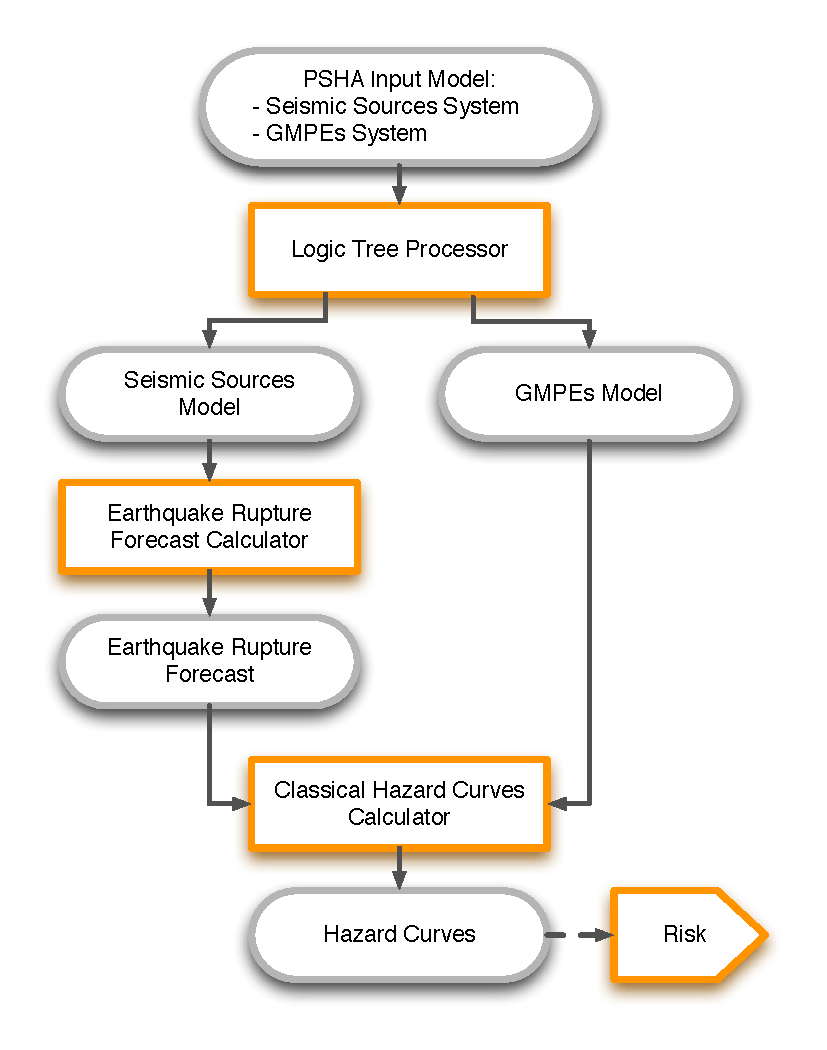
\includegraphics[width=12cm]{./Figures/Part_Hazard/classical_psha_workflow.eps}
\caption{Workflow for classical PSHA (boxes with purple border represent the 
calculators). Given a PSHA Input Model 
the Logic Tree Processor is responsible for creating a Seismic Sources model
and a ground motion model. 
The Seismic Sources model is then provided to the Earthquake Rupture Forecast 
calculator, which computes the ERF (the list of all earthquake ruptures in the 
source model with their probabilities of occurrence). 
Using the ERF and the GMPEs model the Classical PSHA calculator produces 
curves at the sites of interest.}
\label{classical_psha_workflow}
\end{center}
\end{figure}
% . . . . . . . . . . . . . . . . . . . . . . . . . . . . . . . . . . . < Figure
% ..............................................................................

As represented in Figure \ref{classical_psha_workflow}, the main calculators 
used to perform this analysis are:
\begin{enumerate}
%
\item \emph{Logic Tree Processor} \hfill \\
The Logic Tree Processor takes as an input the PSHA Input model. In case of 
the Seismic Sources, using the one of the Initial Seismic Sources Models and 
and by 'harvesting' the information contained in the Seismic Sources Logic Tree
- that is to sample the epistemic uncertainties - it creates a Seismic Sources 
Model (i.e. a model describing geometry and activity rates of each source 
without any epistemic uncertainty). 
%
Following the procedure just described the Logic Tree Processor creates a 
Ground Motion model (i.e. a data structure that associates to each tectonic 
region considered in the calculation a GMPE).
%
\item \emph{Earthquake Rupture Forecast Calculator} \hfill \\
The produced Seismic Sources Model is then used as input for the Earthquake 
Rupture Forecast (ERF) calculator which computes the probability of occurrence, 
over a specified time span, for each earthquake rupture produced by the source 
model.
\item \emph{Classical PSHA Calculator} \hfill \\
The cPSHA uses the ERF and the Ground Motion model to compute hazard curves on 
each site specified in the calculation settings.
\end{enumerate} 
%
%  - - - - - - - - - - - - - - - - - - - - - - - - - - - - - - - - - - - - - - -
\subsection{Event-Based Probabilistic Seismic Hazard Analysis}
\label{section:event-basedPSHA}
Input data for the Event-Based PSHA - as in the case of the Classical PSHA 
calculator - consist of a PSHA Input Model supplied to OQ together with a 
set of calculation settings.
%
% ..............................................................................
% . . . . . . . . . . . . . . . . . . . . . . . . . . . . . . . . . . . > Figure
\begin{figure}
\centering
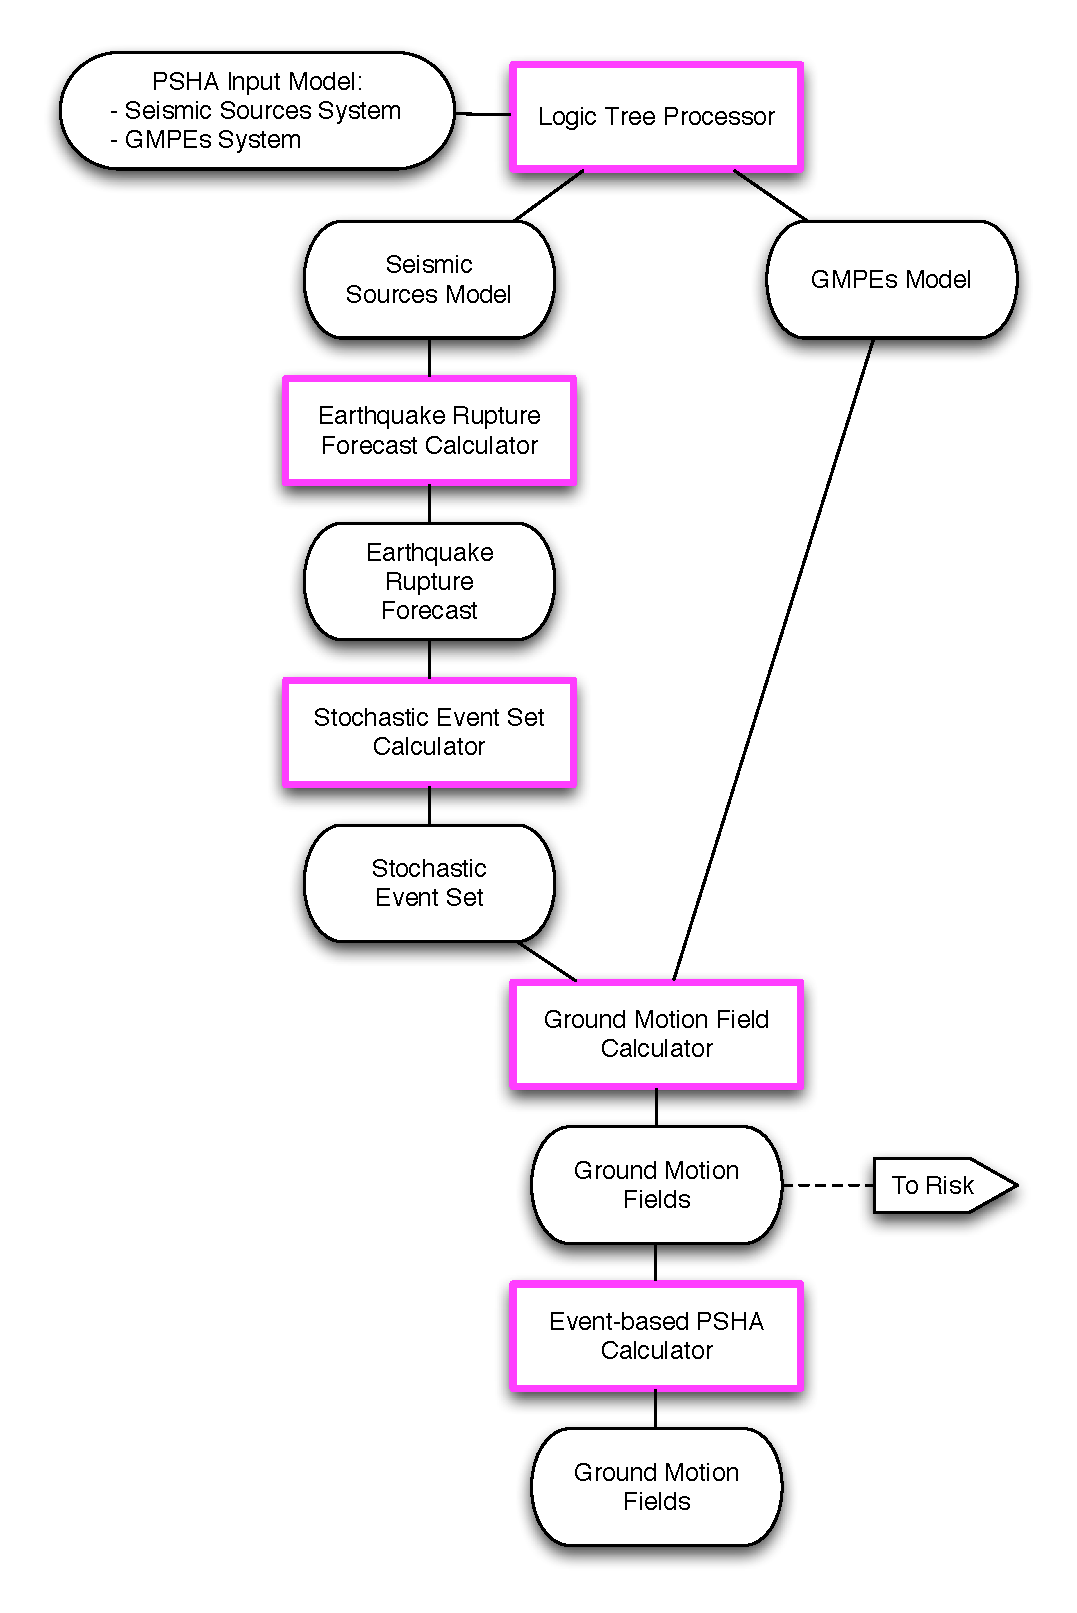
\includegraphics[width=12cm]{./Figures/Part_Hazard/event_based_workflow.eps}
\caption{Workflow for event-based PSHA. Similarly to the classical PSHA workflow 
(Figure \ref{classical_psha_workflow}), an ERF is computed, which is then used 
to generate a stochastic event set (representative of the seismic activity of 
a region in a given time span). Each event is then utilized to calculate a 
ground motion field over a region of interest.}
\label{event_based_workflow}
\end{figure}
% . . . . . . . . . . . . . . . . . . . . . . . . . . . . . . . . . . . < Figure
% ..............................................................................
As represented in Figure \ref{event_based_workflow}, the main calculators 
used to perform this analysis are:
\begin{enumerate}
%
\item \emph{Logic Tree Processor} \hfill \\
The Logic Tree Processor was already 
introduced in the description of the cPSHA workflow (see section 
\ref{section:classicalPSHA} at page \pageref{section:classicalPSHA}).
%
\item \emph{Earthquake Rupture Forecast Calculator} \hfill \\ 
The Logic Tree Processor was already 
introduced in the description of the cPSHA workflow (see section 
\ref{section:classicalPSHA} at page \pageref{section:classicalPSHA}).
%
\item \emph{Stochastic Event Set Calculator} \hfill \\
The Stochastic Event Set Calculator generates a Stochastic Event set 
by sampling each rupture contained in the ERF according to its 
probability of occurrence. Usually a Stochastic Event Set (SES) contains
a large number of seismicity history each one representative of a  
possible collection of events that can be produced by the seismic sources
considered in an analysis during the time span fixed for the calculation
of hazard (normally corresponding to 50 years).
%
\item \emph{Ground Motion Field Calculator} \hfill \\
The Ground Motion Field Calculator computes for each event contained in a 
Stochastic Event Set - provided as an input - a realization of the 
ground shaking taking into account the aleatory uncertainties in 
the ground motion model. Eventually, the Ground Motion Field calculator 
can consider the spatial correlation of the ground motion during the 
generation of the GMF.
%
\item \emph{Event-based PSHA Calculator} \hfill \\
The event-based PSHA calculator takes a (large) set of ground motion 
fields representative of the possible shaking that the investigated 
area can eventually experience over a (large) time span and for each 
grid node in a ground motion fields computes the corresponding hazard 
curve. 
%
This procedure is computationally intensive and is not recommended for 
investigating the hazard over large areas. 
\end{enumerate}

The Logic Tree Processor and the Earthquake rupture forecast were already 
introduced during the descrption of the cPSHA workflow (see section 
\ref{section:classicalPSHA} at page \pageref{section:classicalPSHA}).
%
%  - - - - - - - - - - - - - - - - - - - - - - - - - - - - - - - - - - - - - - -
\subsection{Deterministic Seismic Hazard Analysis}
\label{section:deterministicSHA}
% Deterministic
For deterministic SHA (DSHA), the input data consist of a single earthquake 
rupture model and a single ground motion model. Using the Ground Motion Field 
Calculator, multiple realizations of ground shaking can be computed, each 
realization sampling the aleatory uncertainties in the ground motion model.

As represented in Figure \ref{deterministic_workflow}, the main calculators 
used to perform this analysis are:
\begin{enumerate}
\item \emph{Ground Motion Field Calculator} \hfill \\
The Ground Motion Field Calculator was already 
introduced during the descrption of the ePSHA workflow (see section 
\ref{section:event-basedPSHA} at page \pageref{section:classicalPSHA}).
\end{enumerate}
% ..............................................................................
% . . . . . . . . . . . . . . . . . . . . . . . . . . . . . . . . . . . > Figure
\begin{figure}[!hb]
\centering
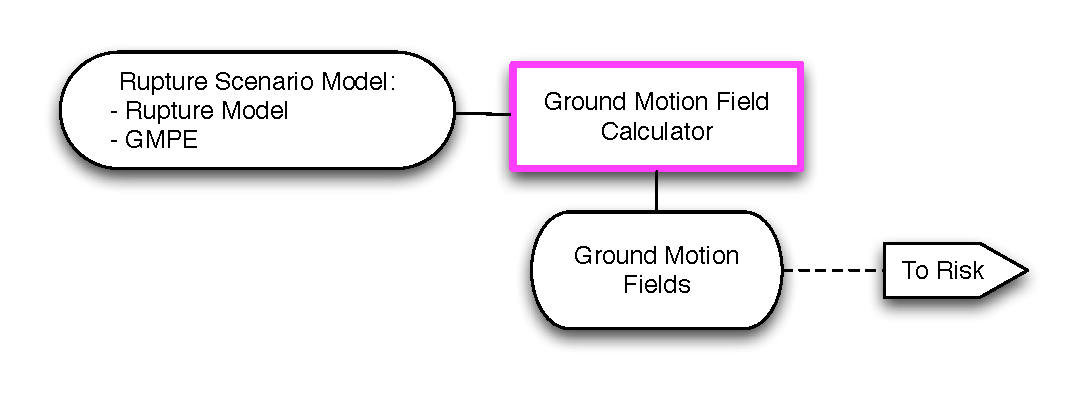
\includegraphics[width=12cm]{./Figures/Part_Hazard/deterministic_workflow.eps}
\caption{Workflow for deterministic SHA. Given a rupture scenario model, 
consisting of an earthquake rupture model, plus a GMPE, the ground motion 
field calculator can compute multiple ground motion field realizations (by 
taking into account GMPE aleatory uncertainties).}
\label{deterministic_workflow}
\end{figure}
% ..............................................................................
% . . . . . . . . . . . . . . . . . . . . . . . . . . . . . . . . . . . > Figure
%
% More details in the next chapters
%Next chapters discuss in more details the data model and the calculators. 
%Chapter \ref{chap:hazinp} describe the input data definition, that is the 
%different options for modeling seismogenic sources and how to include 
%epistemic uncertainties in both seismicity and ground motion models in 
%the form of a logic tree; Chapter \ref{chap:hazinp} also incorporates 
%the description of the logic tree structure adopted. 
%
%The methodology adopted to process the logic tree structure and the 
%definition and modeling of earthquake ruptures for the different 
%seismogenic source typologies are the topics of Chapter \ref{chap:erf}. 
%
%Chapter \ref{chap:hazcalc} describes the theoretical framework behind the main 
%hazard calculator available in OpenQuake: classical PSHA calculator and event 
%based calculator.
% ------------------------------------------------------------------------------
\chapter{OpenQuake Input Description}
	\label{chap:hazinp}
	%
% ------------------------------------------------------------------------------
	\index{PSHA!Input model}
%
OpenQuake requires two main information blocks to perform a calculation: (1) 
a PSHA input model and (2) Calculation Settings.

A PSHA input model defines the properties of the seismic sources 
of engineering  interest within the region considered in the analysis and the 
models capable to describe - once a rupture occurred in a given position - the 
properties of the shaking expected at the site. 
%
A PSHA input model contains two main objects: the \emph{Seismic Sources System} 
and the \emph{Ground Motion Models System}. 
%
The former specifies location, geometry, and seismicity properties of seismic 
sources and potential epistemic uncertainties affecting this information. 
%
The latter describes the details of the ground motion prediction equations to 
be adopted in the calculation and the related epistemic uncertainties. 
%
Therefore, OpenQuake PSHA input models are always defined using two logic 
tree structures, one describing epistemic uncertainties associated with the 
creation of the ERF - called \emph{Seismic Sources logic tree} - 
	\index{Logic Tree!Seismic sources}
the other - called \emph{Ground Motion Models logic tree} - takes into account 
the uncertainties connected with the use of models capable to predict the 
expected ground motion at the site. 
	\index{Logic Tree!Ground Motion Models}
%
In cases where the epistemic uncertainties are not considered, the logic tree 
structure simply consists of one branching level with just one branch (with 
weight equal to 1).

Calculation settings specifies for example the typology of results required,
the site or the sites where to compute the hazard, the methodology to apply.

The organisation of this chapter is the following. The next section offers
further explanations about the way we describe and model logic trees. 
Section \ref{hazard:seismic_source_types} contains a description of the seismic
source type currently supported by OpenQuake while section 
\ref{hazard:seismic_source_types} provides a short description of the 
ground motion models currently supported. Finally, section 
\ref{hazard:calculation_settings} provides an outlook of the hazard 
specific calculation setting supported by OpenQuake.
%
% ------------------------------------------------------------------------------
%
% ------------------------------------------------------------------------------
\section{Logic-tree description}
\label{hazard:logic_tree}
Logic-trees are a tool designed to consider in a systematic manner the 
epistemic uncertainties of models and parameters included in a hazard 
analysis.
% ..............................................................................
% . . . . . . . . . . . . . . . . . . . . . . . . . . . . . . . . . . . > Figure
\renewcommand{\psedge}{\ncdiag[armA=0,angleB=180,armB=1cm]}
\begin{figure}[!hb]
\input{./Part_Hazard/pstricks/sslt_absolute.tex}
\caption{An example of branch set used to account for the epistemic 
uncertainties on faults dip angle; in this case each branch contains a value 
of the dip.}
\label{fig:logic_tree_branching_levels}
\end{figure}
% . . . . . . . . . . . . . . . . . . . . . . . . . . . . . . . . . . . < Figure
% ..............................................................................

A logic tree cont\-ains three main elements:
\begin{itemize}
\item Branching Level
\item Branch Set
\item Branch
\end{itemize}
%
A \emph{branching level}, expresses the distance of a given element from the 
root of the logic tree; in the simplest case each branching level corresponds 
to a single type uncertainty (e.g. maximum magnitude). 
Indicatively, we can say that the larger the number of branching levels in a 
logic structure the larger is its complexity.
%
\index{Logic Tree!Branch set}
A \emph{branch set} describes an uncertainty model; for example - as previously 
mentioned - a model accounting for the epistemic uncertainties connected with 
the definition of maximum magnitude. A branch set contains of a number of 
mutually exclusive and collectively exhaustive options \citep{bommer2008}. 
%
Finally, a \emph{branch} represent a particular alternative in a branch set and 
therefore it refers to an uncertainty model and has a weight expressing - 
according to different interpretations available in the literature 
- ``probabilities or simply subjective indications of relative merit'' 
\citep[][page 999]{bommer2008}.
	\index{Logic Tree!Branch}

%
In more detail, a branch set - the fundamental component in our logic tree data 
model - consists on (1) the parameter (or model) affected 
by uncertainty, (2) the specification of the type of uncertainty (3) the 
listing of the - mutually exclusive and collectively exhaustive 
- alternative hypotheses (4) a weight for each hypothesis, 
(5) a flag specifying if the branches are (totally) correlated and, (6) the 
index of the branches of the previous level - or the subset of seismic 
sources - to which this branch set applies.

Figure \ref{fig:logic_tree_branching_levels} depicts a branch 
set fixing epistemic uncertainties on the dip angle of simple 
fault sources. In this case the possible values of the dip are specified
on each branch composing the branch set (i.e. 30, 45 and 60 degrees). This 
means that these three values are the only ones admitted for all the sources 
included in the initial seismic source model considered. 
%
Figure \ref{fig:logic_tree_branching_levels_1} also shows a branch
set defining epistemic uncertainties on the dip angle 
of simple fault sources. In this case, however, the values specified for each 
branch aren't absolute dip angles but instead differential values to be added - 
or subtracted - to the dip value specified for each simple fault source 
contained in the initial seismic sources model.

% ..............................................................................
% . . . . . . . . . . . . . . . . . . . . . . . . . . . . . . . . . . . > Figure
\renewcommand{\psedge}{\ncdiag[armA=0,angleB=180,armB=1cm]}
\begin{figure}
%\fbox{\begin{minipage}{\textwidth}
\hfill \\
\textcolor{blue01}{\emph{Branch set definition}}: \dotfill
	Simple Fault Dip Angle \\
\textcolor{blue01}{\emph{Branch set uncertainty type}}: \dotfill
	Relative values \\
\textcolor{blue01}{\emph{Applies to}}: \dotfill
	All previous branches \\
\textcolor{blue01}{\emph{Correlated branches}}: \dotfill Yes \\
\hfill \\
	\centering
	\begin{psTree}[treemode=R,levelsep=*2cm]
			{\Tr{ }}
		\begin{psTree}[treemode=R]{
			\Tr{\parbox[b]{4cm}{ value = -15$^\circ$ 
				\newline weight=w$_1$}}}%
		\end{psTree}%
		\begin{psTree}[treemode=R,treenodesize=1cm]{
			\Tr{\parbox[b]{4cm}{ value = 0$^\circ$ 
				\newline weight=w$_2$}}}%
		\end{psTree}%
		\begin{psTree}[treemode=R]{
			\Tr{\parbox[b]{4cm}{ value = +15$^\circ$ 
				\newline weight=w$_3$}}}%
		\end{psTree}%
	\end{psTree}%
\\ \hfill \\
%\end{minipage}} % End of fbox
\caption{An example of branch set used to account for the epistemic 
uncertainties on faults dip angle; in this case each branch contains a 
differential from a default dip value indicated for each source in the 
initial seismic sources model.}
\label{fig:logic_tree_branching_levels_1}
\end{figure}
% . . . . . . . . . . . . . . . . . . . . . . . . . . . . . . . . . . . < Figure
% ..............................................................................
Two or more branch sets they can be combined in flexible fashion (i.e. 
concatenated) to create an entire logic-tree structure.
Figure \ref{fig:logic_tree_schema} shows an example of a logic tree 
created by combining the two branch sets described in the upper part of the
figure. 
The first branch set accounts for epistemic uncertainties connected with 
the dip of simple fault sources whilst the second specifies 
the epistemic uncertainties relative to the depth to the top of rupture  
(this branching level also applies to simple faults included in the model).
% ..............................................................................
% . . . . . . . . . . . . . . . . . . . . . . . . . . . . . . . . . . . > Figure
\begin{figure}[!h]
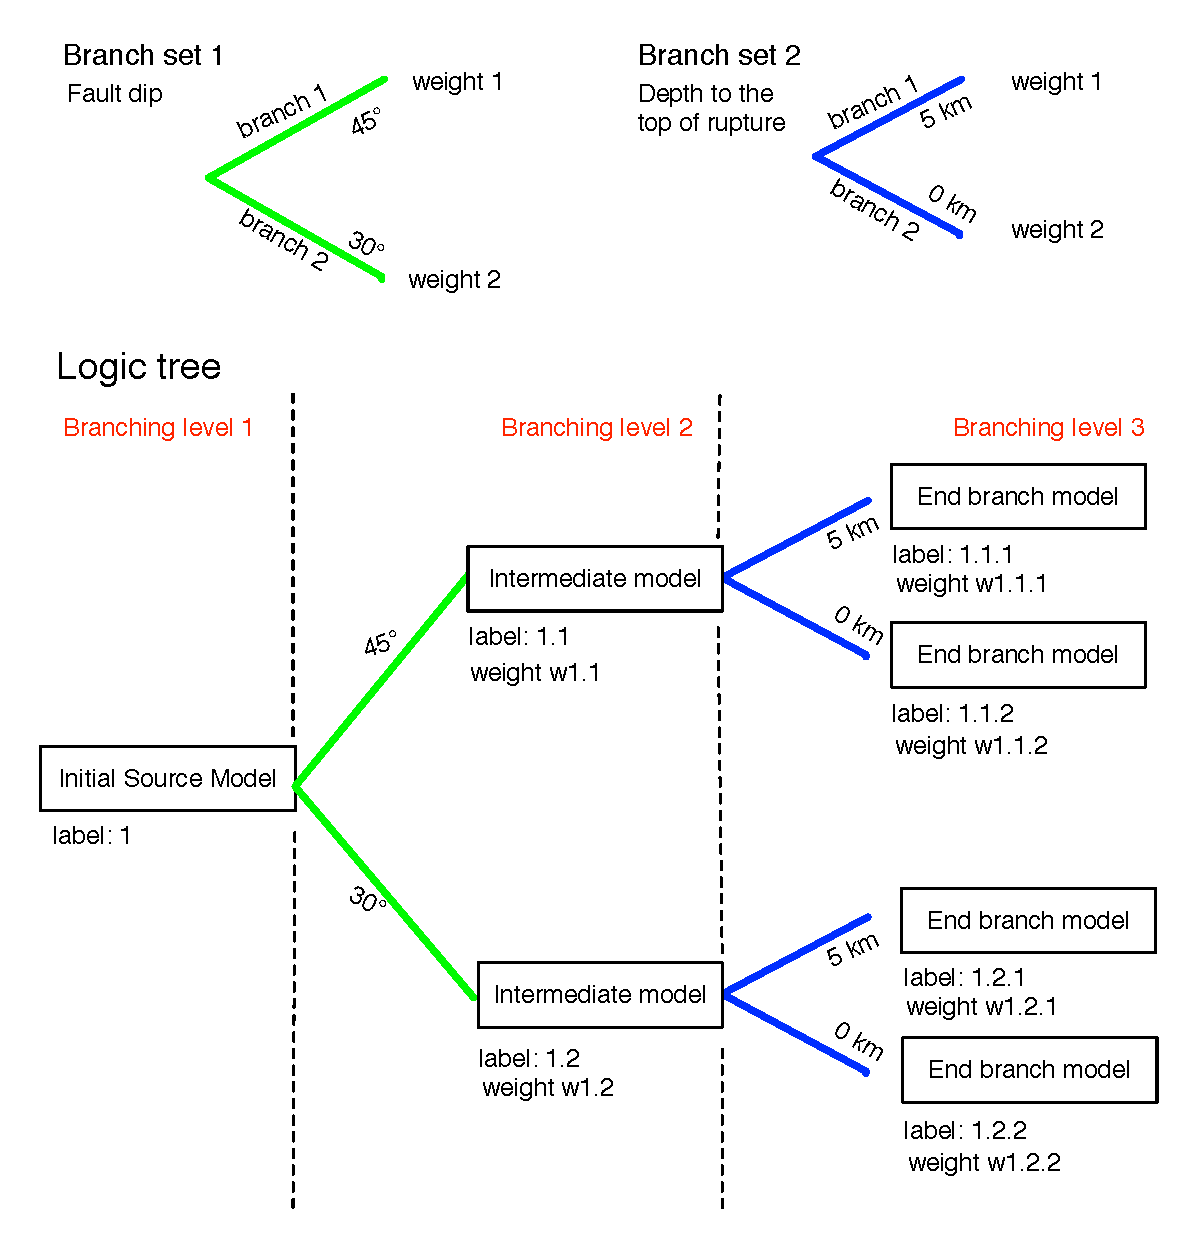
\includegraphics[width=15cm]{./Figures/Part_Hazard/logic_tree_schema.eps}
\caption{Example of a logic tree structure as defined in OpenQuake. The upper
part of the Figure depicts two branch sets.}
\label{fig:logic_tree_schema}
\end{figure}
% . . . . . . . . . . . . . . . . . . . . . . . . . . . . . . . . . . . < Figure
% ..............................................................................
%

This data model permits a very general definitions of logic tree 
structures. For instance, a non-symmetric logic tree can be easily 
created by placing multiple branch sets in the same branching level, each 
branch set being connected to a specific branch of a branch set defined in a
previous branching level. Figure \ref{fig:LogicTreeGeneralStructure}) shows a 
general example of a logic tree structure supported by OpenQuake logic tree 
data model. 

% ..............................................................................
% . . . . . . . . . . . . . . . . . . . . . . . . . . . . . . . . . . . > Figure
\begin{figure}
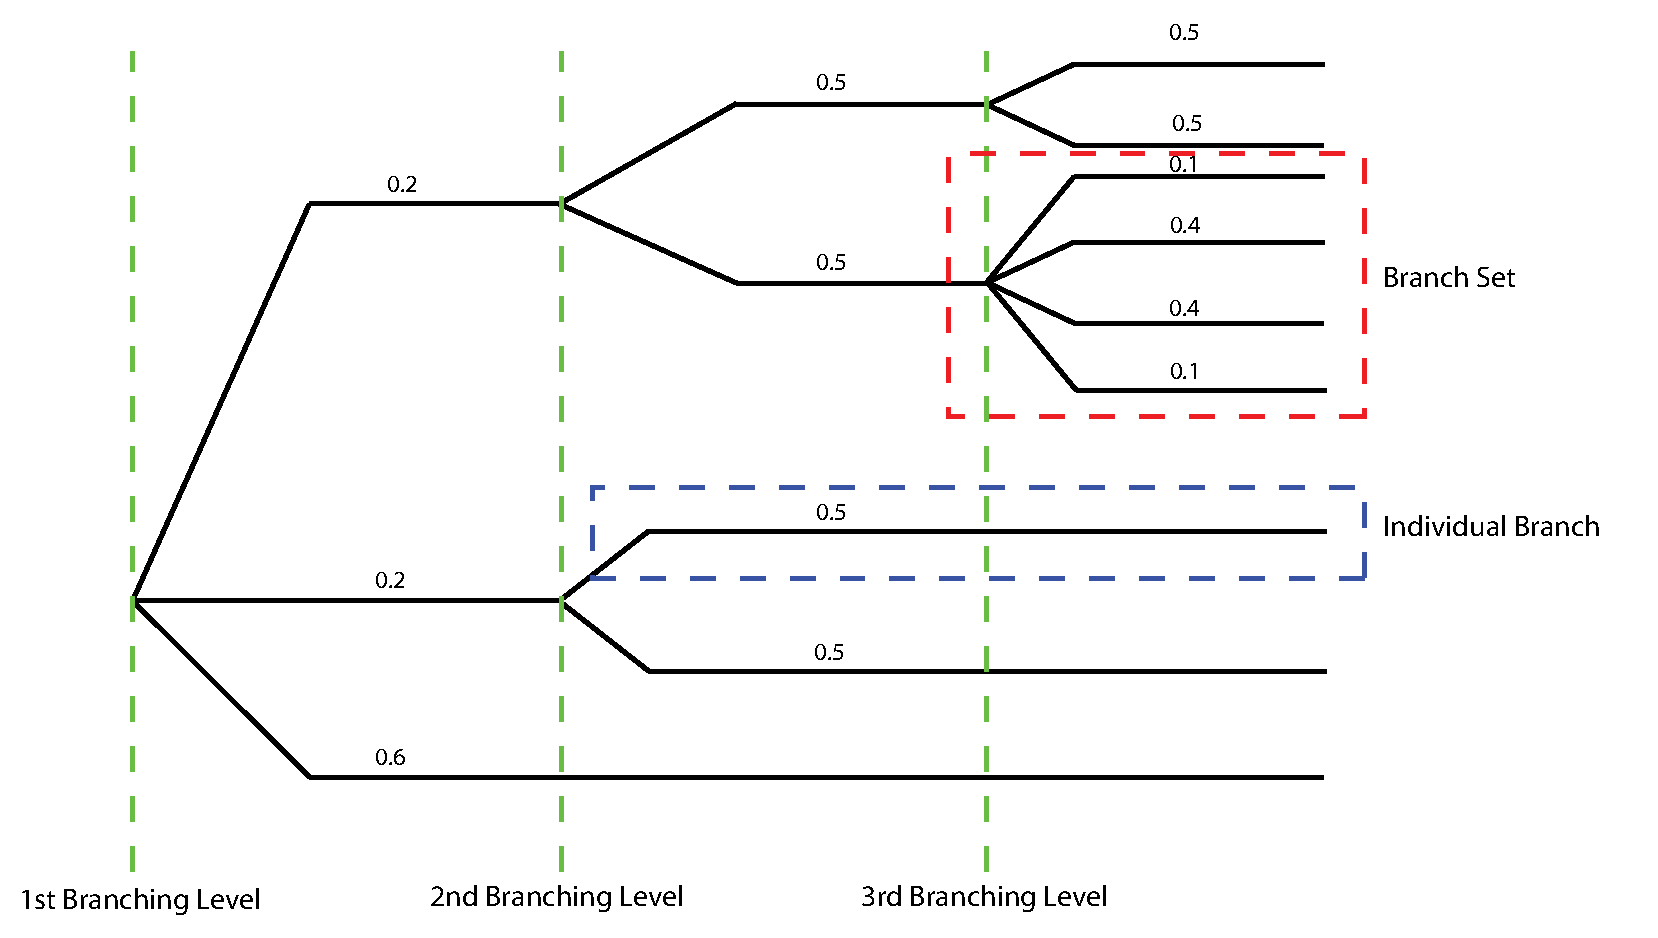
\includegraphics[width=15cm]{./Figures/Part_Hazard/LogicTreeGeneralStructure.eps}
\caption{Logic Tree data structure as defined in terms of individual branches, 
branch sets, and branching levels.}
\label{fig:LogicTreeGeneralStructure}
\end{figure}
% . . . . . . . . . . . . . . . . . . . . . . . . . . . . . . . . . . . < Figure
% ..............................................................................

We use this logic tree description to specify the structure of the Seismic 
Sources Logic Tree as well as for the Ground Motion Models Logic Tree. 
%  - - - - - - - - - - - - - - - - - - - - - - - - - - - - - - - - - - - - - - -
\subsection{Source Model Logic Tree}
\label{hazard:source_model_logic_tree}
%
In the current version of OpenQuake, a seismic sources model logic tree can be 
defined according to the following schema:
\begin{itemize}
\item The first branching level is assumed describing one or more "alternative" 
initial seismic source models.
\item Subsequent branching levels define source parameters uncertainties. 
Parameters uncertainties are applied independently to each seismic source 
in a source model. That is epistemic uncertainties are assumed uncorrelated 
between different seismic sources.
\item One branch set can be defined for branching level, thus assuming 
symmetric logic tree definition only.
\end{itemize}
%
The possibility of defining multiple source models in the first branching 
level responds to the need of modern PSHA of considering alternative source 
models (as derived by different expert opinions, for instance). 
%
Subsequent branching levels define the epistemic uncertainties that 
apply to parameters characterizing seismic sources. The  
epistemic uncertainties related to these parameters are implemented as 
\emph{rules}, that is as algorithms describing how this parameter has to be 
modified. 
%
The major advantage of using a rule-based approach is that a user does not 
need to a provide an input file containing a source model definition 
corresponding to a specific epistemic uncertainty, that is instead computed 
and applied on the fly to the initial model.
%
% ..............................................................................
% . . . . . . . . . . . . . . . . . . . . . . . . . . . . . . . . . . . > Figure
\begin{figure}
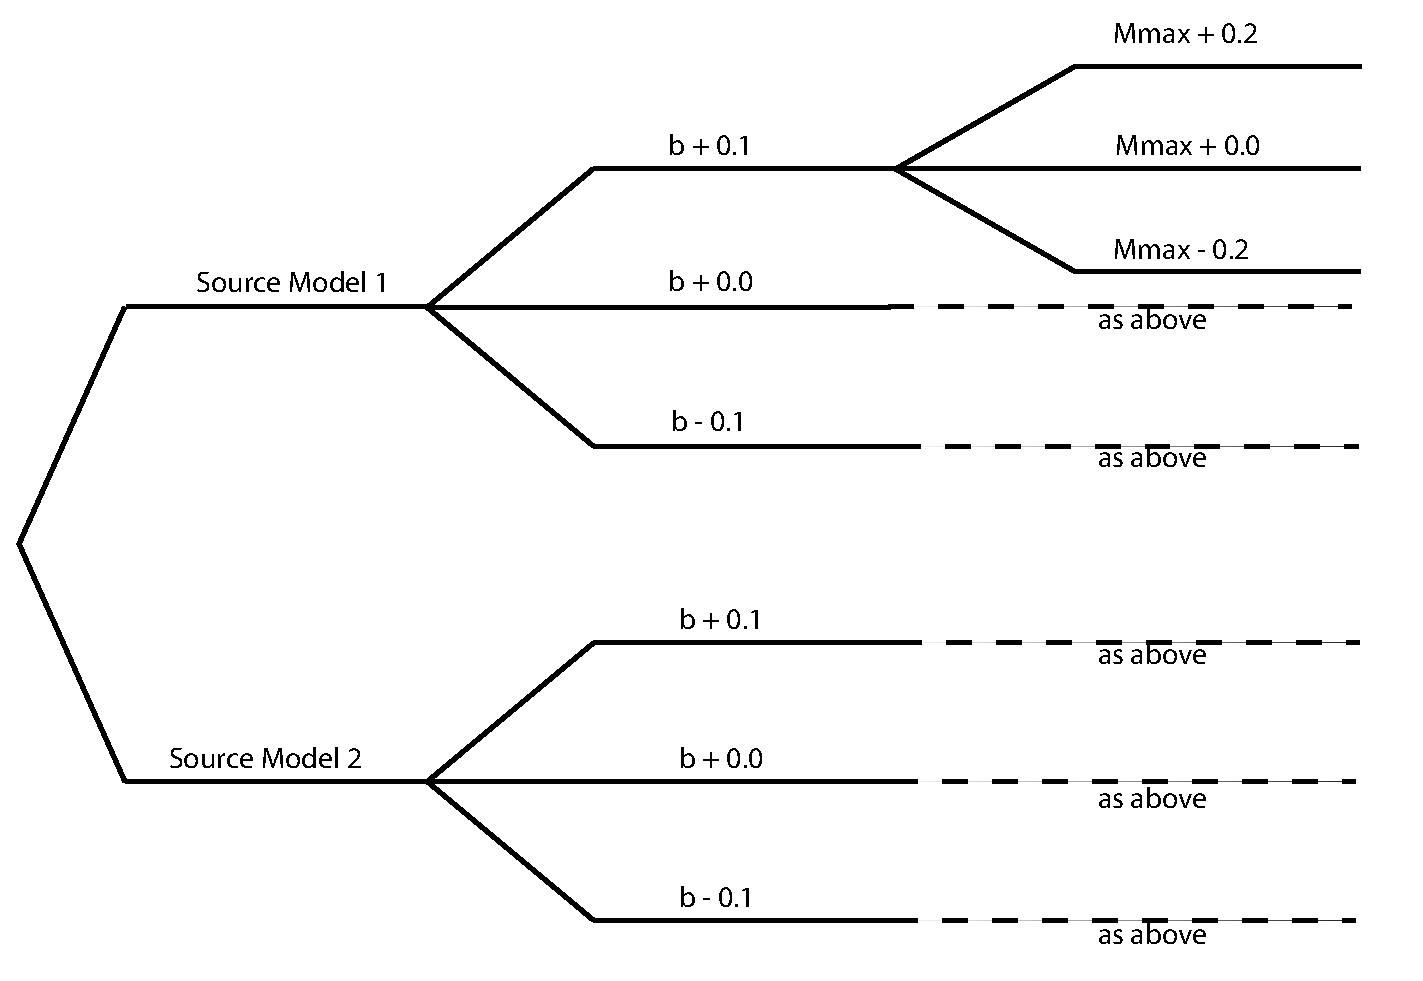
\includegraphics[width=15cm]{./Figures/Part_Hazard/SourceModelLogicTree.eps}
\caption{Example of Seismic Sources Logic Tree. The first branching level defines
two alternative source models (Source Model 1, Source Model 2). The second 
branching level defines uncertainties in b value (increment of 0.1, 0.0, -0.1).
The third branching level defines uncertainties in maximum magnitude 
(increments of 0.2, 0.0, -0.2).}
\label{fig:SourceModelLogicTree}
\end{figure}
% . . . . . . . . . . . . . . . . . . . . . . . . . . . . . . . . . . . < Figure
% ..............................................................................
%

The current version of OpenQuake offers two built-in rules:
\begin{itemize}
\item Gutenberg-Richter b value uncertainties. The user can specify a set 
of increments (positive or negative) that are added to Gutenberg-Richter 
b values. Conservation of total moment rate is assumed.
\item Gutenberg-Richter maximum magnitude uncertainties. The user can specify
a set of increments (positive or negative) that are added to Gutenberg-Richter 
maximum magnitude values. Conservation of total moment rate is assumed.
\end{itemize}
Figure \ref{fig:SourceModelLogicTree} depicts a source model logic tree that 
can be defined with the options currently present in OpenQuake.

The above mentioned rules are only a sample of possible source model epistemic 
uncertainties, and future versions of OpenQuake will provide a broader spectrum
of built-in epistemic uncertainties. Currently, rules are applied to all 
sources. Option to apply rules only to specific sources will be also supported 
in the future.
%  - - - - - - - - - - - - - - - - - - - - - - - - - - - - - - - - - - - - - - -
\subsection{GMPE Logic Tree}
\label{hazard:gmpe_logic_tree}
The GMPE Logic Tree allows a user to consider multiple ground motion prediction
equations in the hazard modeling. Given that GMPEs are often, or can be, 
associated to specific tectonic region types, OpenQuake allows the definition 
of multiple GMPE logic trees, one for each tectonic region type considered in 
the source model. In the current version, a GMPE logic tree can have only one 
branching level, containing only one branch set, where each individual branch 
is associated to a specific GMPE. With the current setting, epistemic 
uncertainties coming from different models can be taken into account, but 
epistemic uncertainties inside each model cannot be captured.
Figure \ref{fig:GMPELogicTree} schematically shows GMPE logic trees that can 
be currently defined in OpenQuake.
% ..............................................................................
% . . . . . . . . . . . . . . . . . . . . . . . . . . . . . . . . . . . > Figure 
\renewcommand{\psedge}{\ncdiag[armA=0,angleB=180,armB=1cm]}
\begin{figure}
\input{./Part_Hazard/pstricks/logicTreeGmpes.tex}
\caption{Examples of GMPE Logic Trees. One for active shallow crust (considering
three GMPEs) and one for subduction interface (considering two GMPEs).}
\label{fig:GMPELogicTree}
\end{figure}

% . . . . . . . . . . . . . . . . . . . . . . . . . . . . . . . . . . . < Figure
% ..............................................................................
\clearpage
% ------------------------------------------------------------------------------
%
% ------------------------------------------------------------------------------
\input{./Part_Hazard/unifiedmodel/seismicSourceTypes.tex}
%
% ------------------------------------------------------------------------------
\section{GMPEs description}
\label{hazard:gmpe_selection}
OpenQuake provides only hardcoded Ground Motion Prediction Equations and misses 
of a mechanisms allowing the user to specify new GMPEs. This is something the 
OpenQuake team may think to introduce in the future. 

For the time being the user in need of a specific Intensity Measure 
Relationship, can:
\begin{itemize}
\item Fork the OpenQuake project from the OQ repository\footnote{The 
OpenQuake software repository can be reached here: 
\hfill \newline  https://github.com/gem/openquake/}, code the new GMPE 
following the examples available in the OpenQuake and OpenSHA repository 
and, - if he's willing to share his contribution with the other OQ users - 
ask to push his modified version of OpenQuake. 
\item Post a ticket on the OpenQuake website \marginpar{this is something 
I need to check with Ben} 
\end{itemize}

Table \ref{tab:OQ_GMPEs} provides a list of the Ground Motion Prediction 
Equations supported. The vast majority are GMPEs implemented in OpenSHA 
with just a couple of developed in the course of the GEM1 project. 
New GMPEs are expected to be added soon with the contribution of 
some GEM's Regional Programmes.
%
\begin{table}[!t]
\centering
\begin{tabular}{llll} \hline
% >>> Table header
\textbf{Ground Motion Prediction} & \textbf{IMTs} & \textbf{Component } & \textbf{ID} \\
\textbf{Equation}& & \textbf{type} & \\ 
\hline
% <<< Table header
\cite{atkinson2006} & PGA & & AtkBoo06 \\
\cite{abrahamson2008} & PGA & & AS2008 \\
\cite{boore2008}  & PGA,PGV,S$_{a}$ & Avg Hor & BA2008 \\
\cite{chiou2008}  & PGA,S$_{a}$ &  & CY2008 \\
\cite{zhao2006}  & PGA,S$_{a}$ &  & ZhaoEtAl2006 \\
\hline
\end{tabular}
\caption{Some of the Ground Motion Prediction Equations (in the OpenSHA 
terminology Intensity Measure Relationship) currently included in OpenSHA 
and OpenQuake.}
\label{tab:OQ_GMPEs}
\end{table}
%
%
% ------------------------------------------------------------------------------
\section{Calculation settings description}
\label{hazard:calculation_settings}
%




% ------------------------------------------------------------------------------
\chapter{The Logic Tree Processor and the Earthquake Rupture Forecast 
	calculator}
	\label{chap:erf}
	In this chapter we discuss the properties of the two main calculators 
needed to process the information contained in the PSHA input model 
and prepare it for hazard calculation: the Logic Tree processor and the 
Earthquake Rupture Forecast calculator. 

\section{The Logic Tree Processor}
\label{hazard:logic_tree_processor}
\index{Logic Tree!Processor}
%
The Logic Tree Processor is responsible for processing data contained in a 
logic tree structure (see \ref{hazard:logic_tree}), that is selecting a 
source model from the source model logic tree (see 
\ref{hazard:source_model_logic_tree}) and a ground motion prediction equation 
from the GMPE logic tree (see \ref{hazard:gmpe_logic_tree}). The selected 
source model and GMPE can be then passed to the different OpenQuake-Hazard 
calculators (Classical PSHA calculator, \ref{chap:classic_psha}; Stochastic 
PSHA calculator, \ref{chap:stochastic_psha}).\\
The capability to process the information contained in a logic tree is 
constrained by the size and complexity of the logic tree itself. For a 
large logic tree, performing a seismic hazard calculation for all possible 
end-branch models is an unfeasible task. Under this condition, a Monte Carlo
sampling of the logic tree is a more efficient approach. On the contrary, 
for a small logic tree, a Monte Carlo approach is inefficient with respect
to enumerating all the possible end-branch models and performing a hazard 
analysis for each of them. In other words, to get stable results in case of 
a simple logic tree,  a Monte Carlo approach would require sampling epistemic
uncertainties a number of times much larger than the actual number of 
end-branch models.\\
The general plan for OpenQuake is to provide both the two processing strategies. 
Currently, the logic tree processor can only provide a Monte Carlo sampler.
%
\subsection{The Logic Tree Monte Carlo Sampler}
Aim of the Logic Tree Monte Carlo Sampler (hereinafter LTMCS) is to sample 
epistemic uncertainties, so that the distribution of the final hazard results
reflect the degrees of belief that the hazard modeler specified in the 
different logic tree branches.\\
%
\subsubsection{Sampling the source model logic tree}
As described in \ref{hazard:source_model_logic_tree}, the first branching 
level in the source model logic tree is used for defining one or more 
alternative source models. Subsequent branches define parameter-specific 
epistemic uncertainties. Each branching level contains only one branch set 
(therefore producing a symmetric logic tree). The LTMCS constructs a source 
model by looping over all the branching levels. In the first branching level, 
a source model is randomly selected, with a probability equal to the 
uncertainty weight. Epistemic uncertainties defined in subsequent branching 
levels are then applied to this initially selected source model. For each 
following branching level, a loop over the seismic sources defined in the 
selected source model is started, and for each seismic source an epistemic 
uncertainty value is randomly selected (again with a probability equal to 
the uncertainty weight).
	%
% ------------------------------------------------------------------------------
\section{The Earthquake Rupture Forecast Calculator}
\index{Seismic Sources!Model}
\index{Seismic Sources!Initial Model}
The \gls{earthquakeruptureforecast} is a fundamental concept in the OpenSHA 
framework \citep{field2003} as well as in the hazard component of OpenQuake.

As explained in the previous Section, the calculation of the \gls{acr:erf} 
in OQ starts from a \gls{seismicsourcemodel} created by the  
\gls{logictreeprocessor}.
%
When epistemic uncertainty is not included in the seismic source 
system there exists a one to one correspondance between the 
\gls{initialseismicsourcemodel} and the \gls{seismicsourcemodel} used 
in the calculation of hazard. In this case, the \gls{logictreeprocessor} 
just duplicates into the \gls{seismicsourcemodel} the information 
included in the \gls{initialseismicsourcemodel}.
%
In more complicated cases, when epistemic uncertainty affects many 
parameters characterizing seismic sources, the \gls{logictreeprocessor} 
generates many \glspl{acr:ssm} so as to explore entirely the space 
of models admitted by our imprecise knowledge.

Independently of the complication of the seismic source logic tree,
the Earthquake Rupture Forecast calculator processes one at a time the 
\glspl{acr:ssm} and creates a list of the ruptures generated by all 
the sources included. 
%
Each rupture in the list is associated with a probability of occurrence 
in the \gls{investigationtime} specified by the user in the calculation 
settings. To produce this results, the earthquake rupture forecast 
calculator treats separately each source typology included in the 
seismic source model. A detailed description of the methodologies 
adopted to create the earthquake rupture forecast for different seismic
source types is provided in the following Sections.

As a final important note: for the time being - OQ supports just sources 
producing seismicity in accordance with a Possion temporal occurrence model.
%
% - - - - - - - - - - - - - - - - - - - - - - - - - - - - - - - - - - - -- - - -
\subsection{ERF creation in case of distributed seismicity}
Open Quake supports two seismic source typologies capable to model 
distributed seismicity: \glspl{areasource} and \glspl{gridsource}.

Area sources are the most traditional source type adopted in PSHA 
analysis since its first introduction at the end of the 1960s. 
%
The works of \cite{frankel1995} and \cite{frankel1997} boosted the 
use of grid sources in probabilistic seismic hazard calculations. 
%
%. . . . . . . . . . . . . . . . . . . . . . . . . . . . . . . . . . . . . . . .
\subsubsection{Area source}
%
The creation of an ERF in case of \glspl{areasource} (see also Section 
\ref{hazard:seismic_source_types:areaSources} at page 
\pageref{hazard:seismic_source_types:areaSources}) requires a 
preliminary step consisting in the discretization of the polygon 
used to delimit the spatial extension of the source. 
%
% . . . . . . . . . . . . . . . . . . . . . . . . . . . . . . . . . . . > Figure
\begin{figure}[!ht]
\centering
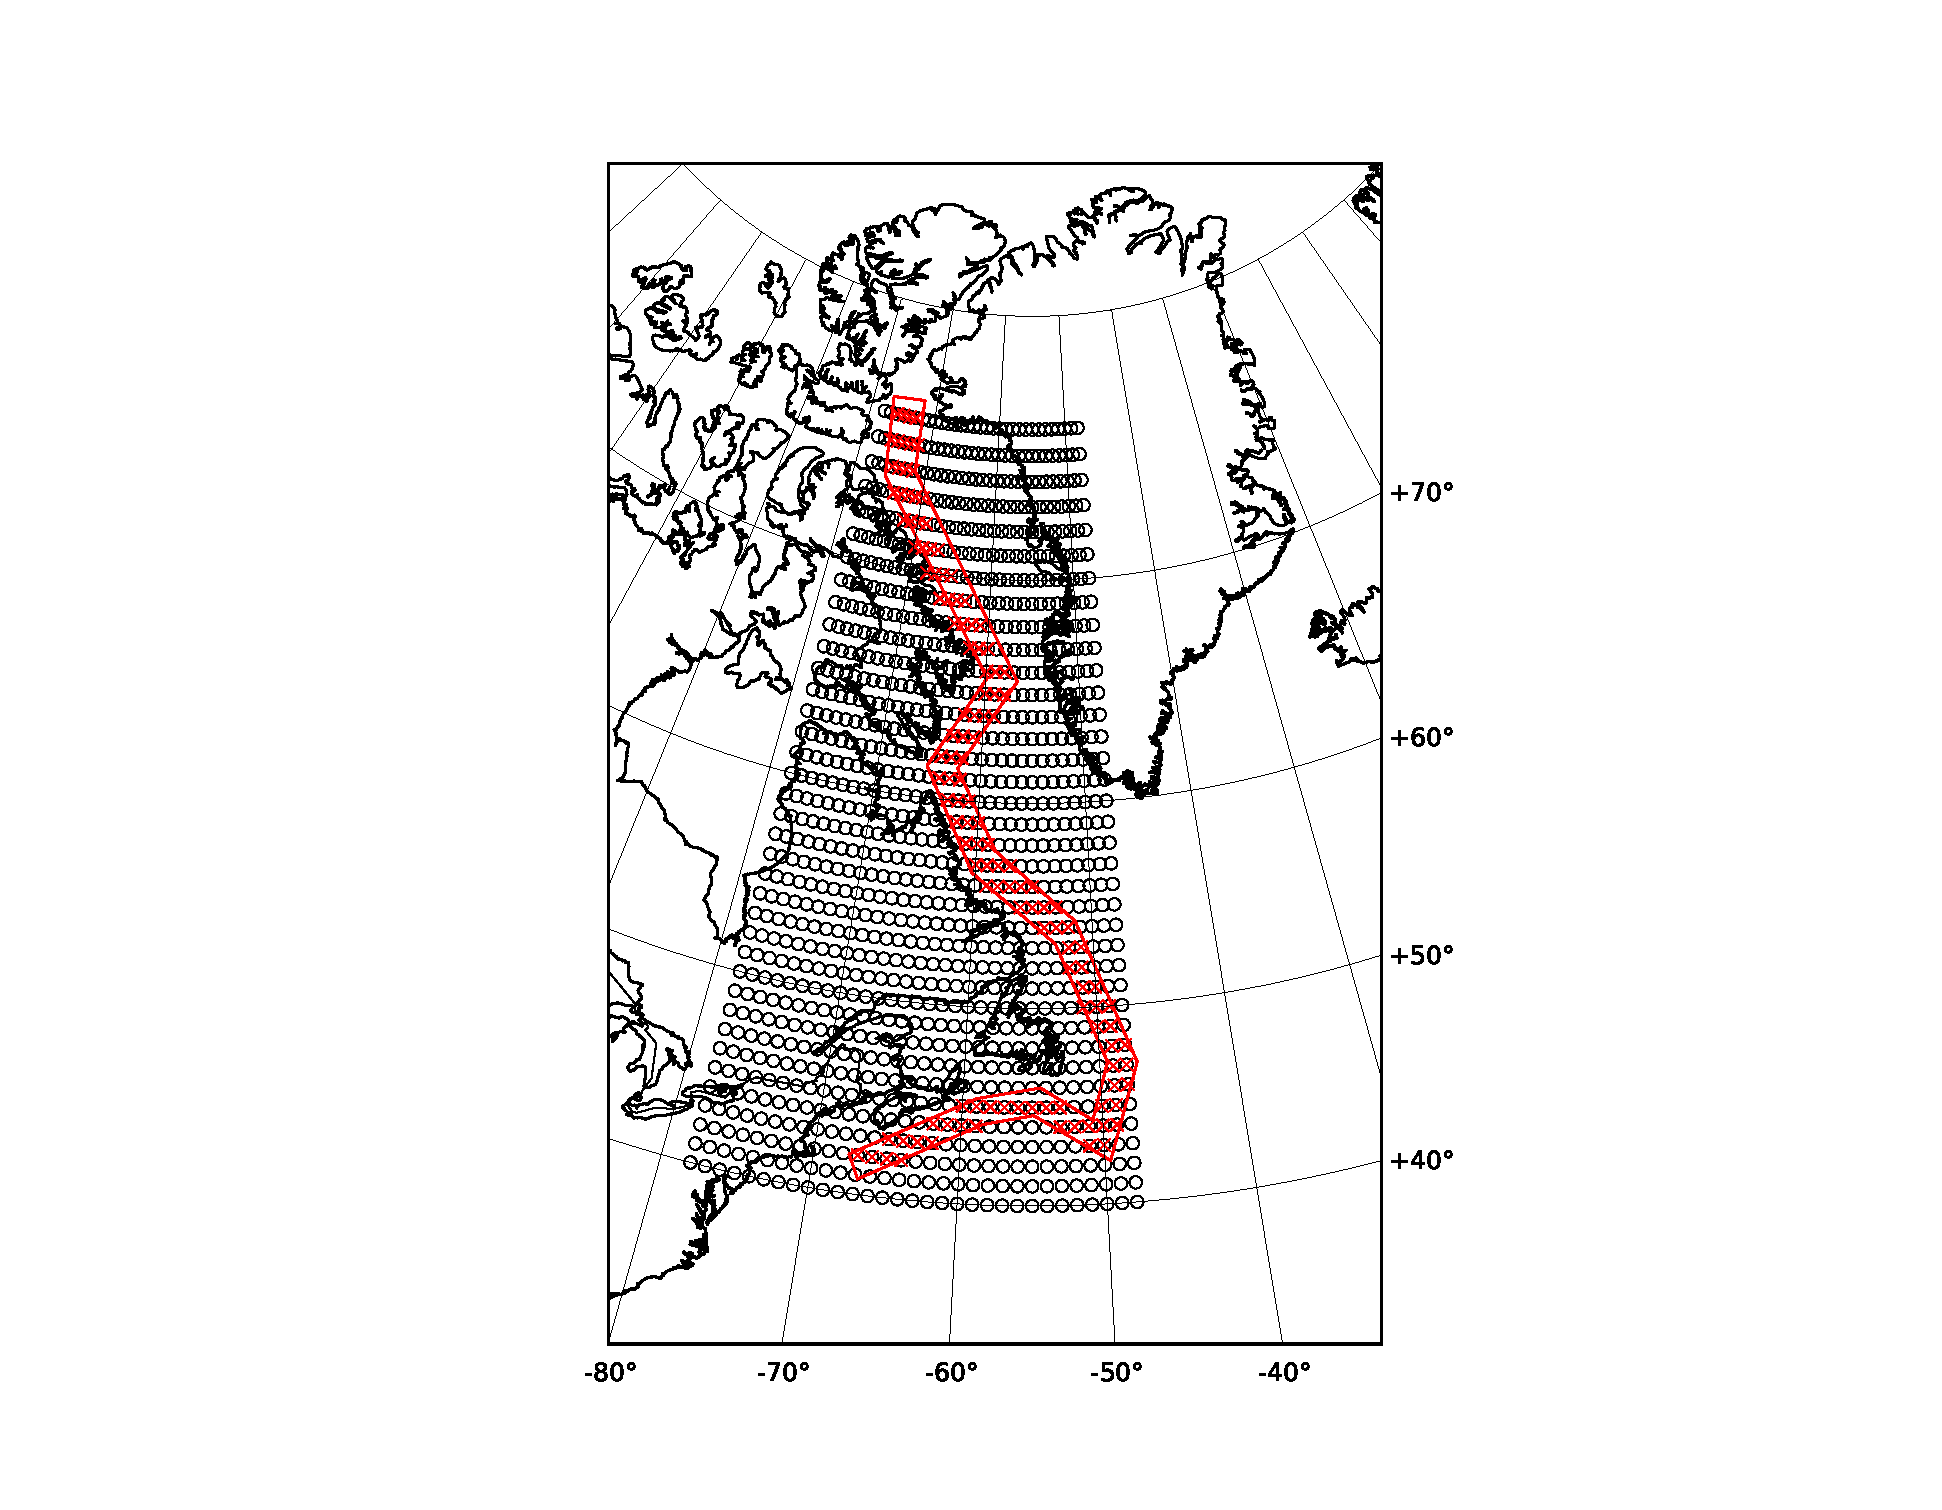
\includegraphics[width=18cm]{./Figures/Part_Hazard/area_source_discretization.eps}
\caption{Example of an area source discretisation (grid spacing equal 
to 0.5$^\circ$). Note how the spacing between circles decreases moving from 
bottom to top of the source.}
\label{fig:area_source_discret}
\end{figure}
% . . . . . . . . . . . . . . . . . . . . . . . . . . . . . . . . . . . < Figure
%
OQ discretizes area sources by overlapping a regular grid of nodes
over the polygon representing the source. The grid contains nodes 
equally spaced in latitude and longitude; the position of each node
is specified by one geographic coordinate, expressed in decimal degrees. 
The nodes of the grid inside the polygon represent - in a discrete way - 
the area source.

The reference system adopted has the advantage that is simple and 
intuitive, however from a computational point of view it has some 
drawback. The most relevant one is that the spacing (in km) between 
nodes of the grid depends on latitude. 
%
Indeed, the spacing of between two nearby nodes near the equator is 
larger than at high latitudes e.g. one degree of longitude at the equator 
correponds to about 111 km, at 45$^\circ$ of latitude it becomes 
about 78.8 km and, at 75$^\circ$ it corresponds to only 28 km. 
%
Figure \ref{fig:area_source_discret} shows a discretization example 
considering an area source contained in the Canada model. If we assume 
the grid nodes as centers of rectangular cells, the shape of these cells
tends to be squeezed as we move towards the poles.

The problem of this uneven distribution of cell size arises when we 
distribute the seismicity defined for the entire area source over the 
nodes used to represent its shape. If the node spacing was homogenous,
the seismicity on each node would be simply the total seismicity divided 
by the number of nodes selected to discretize the area source.
%
In reality this condition is never satisfied, as a consequence, to 
guarantee an homogeneous distribution of seismicity rates \gls{acr:oq} 
we adopt a simple procedure that distributes the seismicity rates 
proportionally to the cell size (i.e grid node spacing).
%
Particularly, for each node of an area source we compute the area using
the following relationship:
\begin{equation}
 \text{area} = 4\pi^2 * \text{grid\_spacing}^2 *  
 	\left(\frac{\text{earth\_radius}}{360}\right)^2 * 
 	\sin(\text{node\_latitude})
 	\label{eq:cell_area}
\end{equation}
where:
\begin{itemize}
\item grid\_spacing is the distance between two consecutive cells 
	of the grid adopted to discretize the area source (a common value 
	adopted to discretize sources is equal to 0.1)
\item earth\_radius is the mean radius of the Earth (approximately 
	6371 km) 
\item node\_latitude is the latitude of the cell of which we compute
	the area.
\end{itemize}
%
To get the seismicity rates for a single grid node we multiply the 
ratio between the area (computed using equation \ref{eq:cell_area}) and 
the area of the entire source (i.e. the sum of the areas computed 
with looping for the grid nodes used to discretize the source polygon).
%
%. . . . . . . . . . . . . . . . . . . . . . . . . . . . . . . . . . . . . . . .
\subsubsection{Multi-depth area source}
%
This source typology is an extension of the just described area source, 
it allows to distribute seismicity within a volume delimited by the 
projection of a polygon lying on the topographic surface along the 
depth-axis and two planes parallel to the topographic surface 
identifying the upper and lower seismogenic depth.

The creation of the \gls{acr:erf} in case of multi-depth area sources
follows the same criteria discussed in the previous section for area
sources. The \gls{acr:fmd} for the entire source is distributed over 
the nodes of the 3D grid used to describe the multi-depth volume.
%
%. . . . . . . . . . . . . . . . . . . . . . . . . . . . . . . . . . . . . . . .
\subsubsection{Grid source}
\Glspl{gridsource} are a source typology that's becoming a valuable alternative
to area sources when modeling distributed seismicity. 
%
The main advantage of grid sources consists on the seismicity smoothing 
procedure that's laying behind their calculation. Seismicity smoothing 
indeed is an objective methodology, reproducible and - usually - not
particularly complex. 

The creation of the ERF in case of \glspl{gridsource} follows the same 
concepts described in the previous section in case of area sources. 
%
The main difference is that with this source type the discretisation step 
is not needed.

%- - - - - - - - - - - - - - - - - - - - - - - - - - - - - - - - - - - - - - - -
\subsubsection{Accounting for rupture finiteness in case of distributed 
seismicity}
%
Each node used to discretise an area source or a multi-depth area 
source or belonging to a grid source has tuples composed by 
the following objects:
\begin{itemize}
\item A discrete representation of a \gls{acr:fmd} 
\item A faulting style, that is strike [optional], dip [optional] and 
rake [optional] 
\end{itemize}
The definition of one, or several, faulting styles is optional; this 
means that in the simplest case only one discrete FMD is specified.

%The \gls{earthquakeruptureforecastcalculator} operates in agreement with
%the parameters specifying the properties of each single node composing
%a seismic source:
%\begin{enumerate}
%\item If no faulting style parameters are specified:
%	\begin{enumerate}
%	\item If the finiteness of the ruptures has to be considered in the 
%	calculation (at least for a given specific magnitude range)
%	\end{enumerate}
%\item If only strike is specified:
%	\begin{enumerate}
%	\item If the finiteness of the ruptures has to be considered in the 
%	calculation (at least for a given specific magnitude range)
%	\end{enumerate}
%\item If strike and rake are specified:
%	\begin{enumerate}
%	\item If the finiteness of the ruptures has to be considered in the 
%	calculation (at least for a given specific magnitude range)
%	\end{enumerate}
%\item If strike, dip and rake are specified:
%	\begin{enumerate}
%	\item If the finiteness of the ruptures has to be considered in the 
%	calculation (at least for a given specific magnitude range)
%	\end{enumerate}
%\item
%\end{enumerate}
%%

% - - - - - - - - - - - - - - - - - - - - - - - - - - - - - - - - - - - - - - - 
\clearpage
\subsection{ERF creation in case of Fault sources}

%
%. . . . . . . . . . . . . . . . . . . . . . . . . . . . . . . . . . . . . . . .
\subsubsection{Fault sources with simple geometry}
Simple faults in OQ are representations of tectonic structures with a . 
The methodology adopted fot the creation of the fault surface uses the 
fault trace, a representative dip direction (e.g. it could be the mean 
dip direction) and, the upper and lower seismogenic depth. 

%
%. . . . . . . . . . . . . . . . . . . . . . . . . . . . . . . . . . . . . . . .
\subsubsection{Fault sources with complex geometry}

%
%. . . . . . . . . . . . . . . . . . . . . . . . . . . . . . . . . . . . . . . .
\subsubsection{Computing the probability of occurrence of each rupture}
In OQ, by convention, we describe the frequency-magnitude distribution using 
a discrete representation. 
This choice offers the largest flexibility in describing the rate of 
earthquakes with respect to magnitude. 
%
% . . . . . . . . . . . . . . . . . . . . . . . . . . . . . . . . . . . > Figure
\begin{figure}[!ht]
\includegraphics[width=15cm]{./Figures/Part_Hazard/gr_example.eps}
\caption{Example of a discrete incremental frequency-magnitude Gutenberg-Richter distribution}
\label{fig:gr-example}
\end{figure}
% . . . . . . . . . . . . . . . . . . . . . . . . . . . . . . . . . . . < Figure
%


% ------------------------------------------------------------------------------
\chapter{SHA Calculators}
	\label{chap:hazcalc}
	\section{OpenQuake Hazard: main concepts}
% Three types of analysis
The OpenQuake-Hazard module offers the capability to perform seismic hazard analysis (SHA) following various approaches. Currently (OpenQuake v 0.3), three main types of analysis are supported:
\begin{itemize}
\item \textbf{Classical probabilistic SHA}, allowing calculation of hazard curves and hazard maps  following classical integration procedure (\cite{cornell1968}) as formulated by \cite{field2003}.
\item \textbf{Event-Based probabilistic SHA}, allowing calculation of ground motion fields from stochastic event sets.
\item \textbf{Deterministic SHA}, allowing calculation of ground motion fields from single earthquake rupture scenario.
\end{itemize}
Each type of analysis involves a number of calculators, each responsible for a specific task. Figures \ref{classical_psha_workflow}, \ref{event_based_workflow}, and \ref{deterministic_workflow} schematically depict the different calculation workflows.\\
% Classical and Event based : Input Data Definition
For both the the classical and event-based probabilistic SHA (hereinafter PSHA), the input data consist of a seismic hazard model structured in terms of a source model logic tree (representing the seismicity model and the associated epistemic uncertainties) and a ground motion model logic tree (representing the ground motion model utilized for ground shaking estimation and the associated epistemic uncertainties).\\
% Seismicity Model
A seismicity model consists of a collection of seismogenic sources. A seismogenic source can be one of four typologies: area, point, simple fault, and complex fault. An area source represents a geographic region where seismicity is assumed to be uniform. A point source models a single geographical location of concentrated seismicity. A collection of point sources or area sources can be used to model distributed seismicity. Seismicity occurring on recognized fault structures can be modeled in terms of simple fault (for a geometrically regular-shaped fault), or as complex fault (allowing modeling of a more geometrically irregular fault structure). Each seismogenic source is also associated to a tectonic region type.\\
% Ground Motion Model
A ground motion model is defined as a collection of ground motion prediction equations (GMPEs), each one associated to a specific tectonic region type (for instance: shallow active crust, stable continental region, subduction interface, subduction intraslab, volcanic). The definition of a tectonic region type allows linking a seismogenic source with the appropriate GMPE.\\
% Epistemic uncertainties
Epistemic uncertainties in the source model...
% Logic Tree processor
Such data is then passed to the Logic Tree Processor that is responsible for 'harvesting' the information contained in the logic tree structure, that is to sample the epistemic uncertainties so that the distribution of the final hazard results reflect the uncertainties in the seismicity and ground motion models. Once a source model is selected from the logic tree, it is subsequently used as input for the Earthquake Rupture Forecast (ERF) calculator which computes the probability of occurrence, over a specified time span, for each earthquake rupture contained in the source model. Such inventory of all the ruptures defined in the source model, with their probabilities of occurrence, is referred to as ERF.\\
When performing a classical PSHA, the ERF is provided as input (together with a ground motion model) to the the Hazard Curve Calculator which compute probabilities of exceeding a set of ground motion values (that is an hazard curve) by summing the contribution from all the earthquake ruptures contained in the ERF. For the event-based PSHA instead, the Stochastic Event Set Calculator generates stochastic event sets by sampling each rupture contained in the ERF according to its probability of occurrence. For each event in the event set, the Ground Motion Field Calculator computes a realization of the ground shaking taking into account the aleatory uncertainties in the ground motion model.\\ 
% Deterministic
For deterministic SHA (DSHA), the input data consist of a single earthquake rupture model and a single ground motion model. Using the Ground Motion Field Calculator, multiple realizations of ground shaking can be computed, each realization sampling the aleatory uncertainties in the ground motion model.\\
% Modular structure
Each type of analysis has a modular structure, thus providing the capability of investigating all possible intermediate results. Moreover, each calculator can be expanded independently so that more calculation options/methodologies can be easily introduced, without affecting the overall calculation workflow.\\
% More details in the next chapters
Next chapters discuss in more details the data model and the calculators. Chapter \ref{chap:idd} describe the input data definition, that is the different options for modeling seismogenic sources and how to include epistemic uncertainties in both seismicity and ground motion models in the form of a logic tree. The inclusion of epistemic uncertainties in the hazard calculations is described in Chapter \ref{chap:ltp}. The definition and modeling of earthquake ruptures for the different seismogenic source typologies is the topic of Chapter \ref{chap:erfc}. Chapter \ref{chap:hcc} describes the theoretical framework behind the hazard curve calculator. The main calculators for the event-based PSHA are described in Chapters \ref{chap:sesc} and \ref{chap:gmfc} (Stochastic Event Set Calculator, and Ground Motion Field Calculator respectively). Examples of classical PSHA, event-based PSHA, and DSHA are reported in Chapters \ref{chap:cpsha}, \ref{chap:ebpsah}, and \ref{chap:dsha}.
\begin{figure}[htbp]
\begin{center}
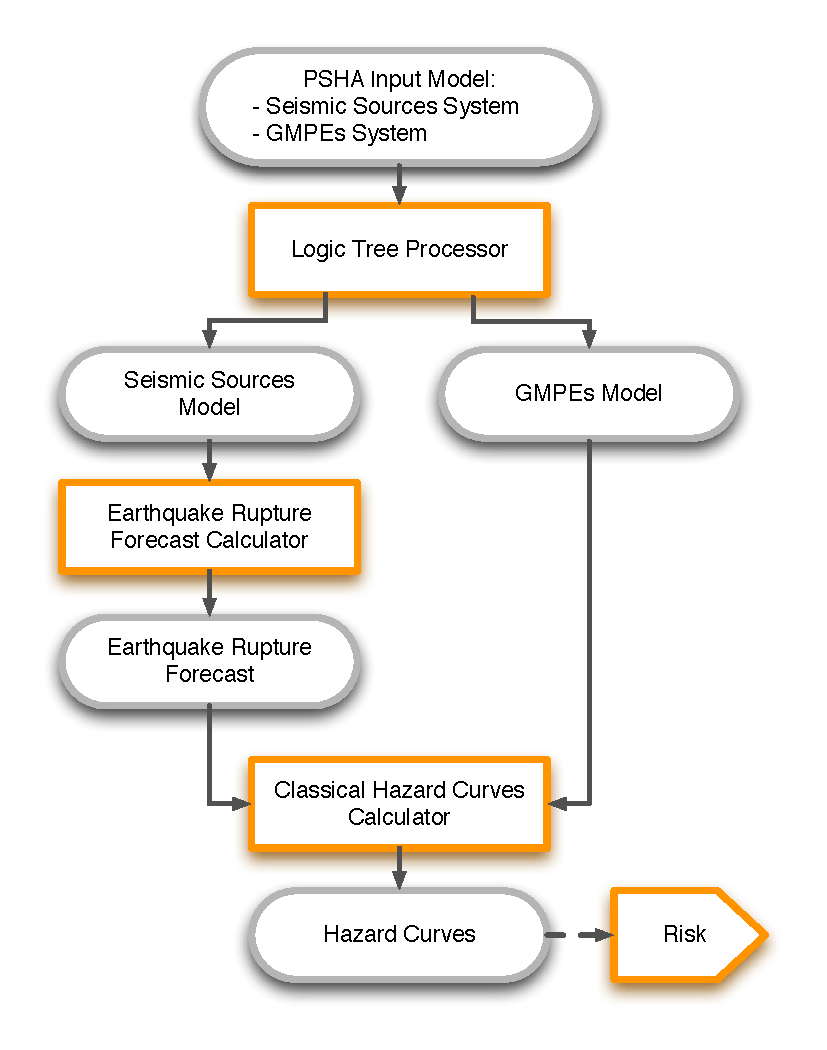
\includegraphics[width=10cm]{./Figures/Part_Hazard/classical_psha_workflow.eps}
\caption{Workflow for classical PSHA. Given a seismic hazard model (expressed as source and ground motion model logic trees), the Logic Tree Processor is responsible for selecting a particular source and ground motion models. The source model is then provided to the Earthquake Rupture Forecast calculator, which computes the ERF (the list of all earthquake ruptures in the source model with their probabilities of occurrence). Together with the selected GMPE hazard curves are calculated.}
\label{classical_psha_workflow}
\end{center}
\end{figure}
\begin{figure}[htbp]
\begin{center}
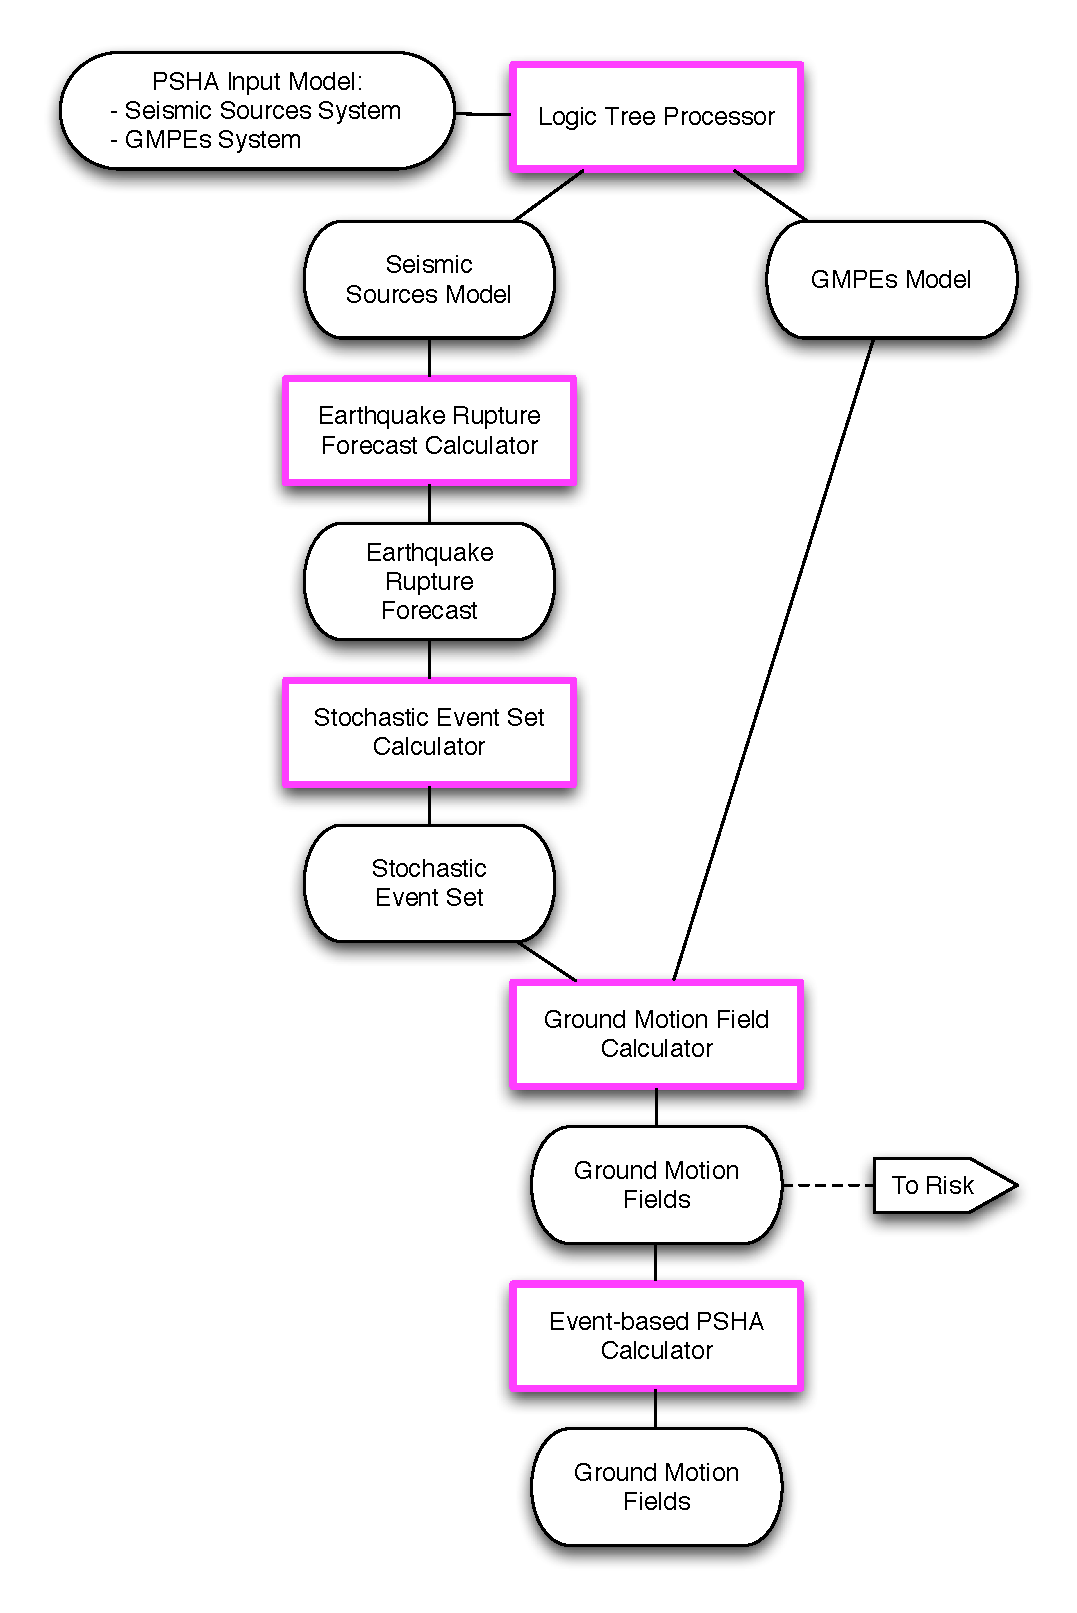
\includegraphics[width=7cm]{./Figures/Part_Hazard/event_based_workflow.eps}
\caption{Workflow for event-based PSHA. Similarly to the classical PSHA workflow (Figure \ref{classical_psha_workflow}), an ERF is computed, which is then used to generate a stochastic event set (representative of the seismic activity of a region in a given time span). Each event is then utilized to calculate a ground motion field over a region of interest.}
\label{event_based_workflow}
\end{center}
\end{figure}
\begin{figure}[htbp]
\begin{center}
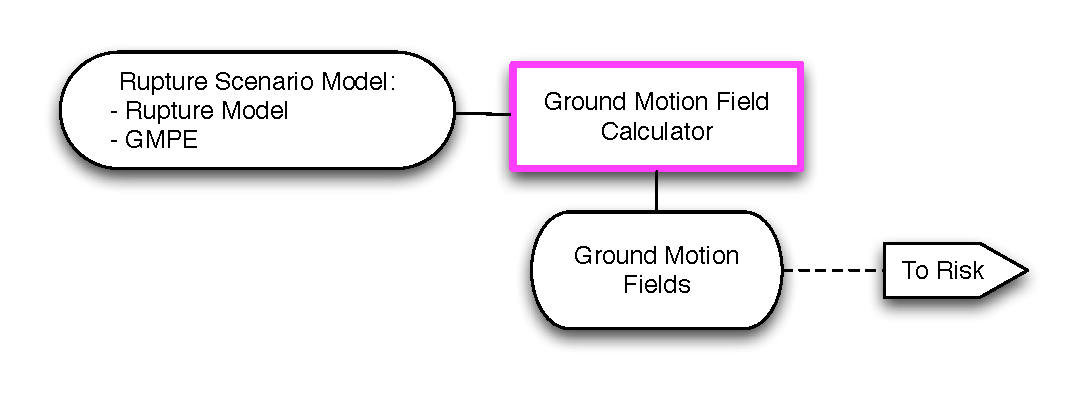
\includegraphics[width=7cm]{./Figures/Part_Hazard/deterministic_workflow.eps}
\caption{Workflow for deterministic SHA. Given a rupture scenario model, consisting of an earthquake rupture model, plus a GMPE, the ground motion field calculator can compute multiple ground motion field realizations (by taking into account GMPE aleatory uncertainties).}
\label{deterministic_workflow}
\end{center}
\end{figure}


	%-------------------------------------------------------------------------------
\section{Classical PSHA calculator}
\label{chap:classic_psha}
%
This calculation methodology is the one we consider the most efficient 
for the calculation of traditional PSHA results such as hazard maps,
hazard curves and uniform hazard spectra.
%
The classical PSHA calculation kernel \citep{field2003} takes as 
input the following information: 
%
\begin{itemize}
\item An \gls{earthquakeruptureforecast} 
\item A \gls{groundmotionmodel} 
\end{itemize}
%
%- - - - - - - - - - - - - - - - - - - - - - - - - - - - - - - - - - - - - - - -
\subsection{PSHA calculation: assuming a negligible contribution from 
repeated ruptures in $t$}
%
The classical PSHA calculation methodology available in OpenQuake 
is the one currently implemented in \gls{opensha}; this methodology
works in terms of probabilities instead of occurrences as many of 
the currently available PSHA codes currently do. 
%
As demonstrated by \citet{field2003}, this method is coherent 
with the classical one under the assumption that the contribution 
to hazard coming from multiple ruptures is negligible (i.e. 
the probability that $src$ will repeat two - or more - $rup$ in $t$ 
is very very low). 

The calculation of hazard for a single site $site$ and a single 
ground-motion parameter $y$ simply consists of an iterative procedure 
that integrates the contributions coming from the ruptures included in 
the \gls{acr:erf} and located at a distance from the $site$ shorter 
than a threshold value (often set in the range 200 to 300 km). 
%
During each iteration, OQ takes a rupture $rup$ within source $src$ and
calculates the probability of exceedance of $y$ in a investigation in 
time $t$ at $site$ using the following equation:
\begin{equation}
P(Y \geq y|t,rup_{src},site) = 
	P(rup_{src}|t)\,
	P(Y\geq y|rup_{src},site)
\label{eq:prob_y_ex_one_rup}
\end{equation}
\marginpar{Check if this equation is formally correct}
The probability $P(Y \geq y|t,rup_{src},site)$ corresponds to 
the product between the probability of occurrence of $rup$ in a time 
$t$ and the conditional probability of exceeding $y$ at $site$ 
given the occurrence of $rup$. 
%
This conditional probability is usually computed by means of a 
\gls{groundmotionpredictioneq} which provides, given a rupture 
and a site, the first two moments of a gaussian distribution 
(a general and common assumption in the ground-motion community). 
\marginpar{here we need a citation}
%
On the contrary, $P(rup_{src}|t)$ is the probability of occurrence 
attributed to $rup$ during the creation of the 
\gls{earthquakeruptureforecast}.
Equation \ref{eq:prob_y_ex_one_rup} can also be rewritten by 
substituting to each rupture the corresponding magnitude and 
node within source $src$.
\begin{equation}
P(Y \geq y|t,m,node_{src},site) = 
	P(m,node|t)\,
	P(Y\geq y|m,node_{src},site)
\end{equation}
This equation states that the probability of exceedance of $y$ in $t$
corresponds to the product between the probability of occurrence
of magnitude $m$ on node $node$ (in OpenSHA and OQ sources are always 
discretized in a number of nodes) and the probability of exceedance of
$y$ given the occurrence of $m$ on $node$. 

Assuming that ruptures within a source are mutually exclusive, 
the probability $P(Y\geq y|t,src,site)$ that at least one rupture 
generated by source $src$ will produce during the investigation 
time $t$ at least one exceedance of $y$, corresponds to the 
difference between unity and the probability that none of the 
ruptures will generate an exceedence of $y$ in $t$.
\begin{equation}
P(Y\geq y|t,src,site) = 1 - \sum_{\forall\,rup\,\text{in}\,src}^{} 
	\Big( P(rup_{src}|t)\,
	P(Y\geq y|rup_{src},site) \Big)
\label{eq:class_psha_1}
\end{equation}
The final value of hazard at site $site$ will be obtained by 
merging the contributions coming from the totality of sources 
considered during the creation of the \gls{acr:erf}, under the 
assumption that events occurring within different sources are 
independent.
%
\begin{equation}
P(Y \geq y|t,site) = 1 - \prod_{\forall\,src\,\text{in}\,ERF}^{} 
\Big( 1-P(Y\geq y|t,src,site) \Big) \label{eq:class_psha_2}
\end{equation}
%
Combining equations \ref{eq:class_psha_1} and \ref{eq:class_psha_2} 
we get \cite[see also][equation 4, page 410]{field2003}:
%
\begin{multline}
P(Y \geq y|t,site) = \\
	1-\prod\limits_{\forall\,src\,\text{in}\,ERF}^{}  
	\left\{
		1-\sum\limits_{\forall\,rup\,\text{in}\,src}^{} 
			\biggl[ P(rup_{src}|t)\,P(Y\geq y|rup_{src},site)
			\biggr]
	\right\}
\label{eq:PSHA_calc_classical_no_repeating}
\end{multline}
%
%- - - - - - - - - - - - - - - - - - - - - - - - - - - - - - - - - - - - - - - -
\subsection{PSHA calculation: accounting for contributions from 
repeated ruptures in $t$}
%
Sometimes  (e.g. in case of particular time dependent PSHAs) the 
assumption of negligible contributions to the final value 
of hazard coming from repeated ruptures does not hold anymore (e.g. in 
case of particular time dependent PSHAs). 
%
Consequently, for precise hazard calculations is necessary to take 
into account any possible contribution produced by the sources in the
\gls{earthquakeruptureforecast}.

In particular, in order to account for repeated ruptures equation 
\ref{eq:prob_y_ex_one_rup} must be rewritten as 
\begin{multline}
P(Y \geq y|t,rup_{src}^{*},site) = \\
	\sum\limits_{n=1}^{\infty}
	\bigl( {1 - P(Y\geq y|rup_{src},site)^{n}}\bigr)
	P(\#rup_{src}=n|t)\,
\label{eq:prob_y_ex_many_rup}
\end{multline}
where $P(Y \geq y|t,rup_{src}^*,site)$ stands for the 
probability of at least one exceedance of $y$ given one or several 
ruptures $rup_{src}$ occurring within source $src$.
% 
As a result, equation \ref{eq:class_psha_1} becomes 
\begin{multline}
P(Y \geq y|t,src,site) = \\
1 - \sum_{\forall\,rup\,\in\,src}^{} 
	\biggl(\,
	\sum\limits_{n=1}^{\infty}
	1 - P(Y\geq y|rup_{src},site))^{n}\bigr)
	P(\#rup_{src}=n|t)
	\biggr)
\end{multline}
%
Substituting equation \ref{eq:prob_y_ex_many_rup} into equation 
\ref{eq:PSHA_calc_classical_no_repeating}
\begin{multline}
P(Y \geq y|t,site) = \\
	1-\prod\limits_{\forall\,src\,\text{in}\,ERF}^{}
	\left\{
		1-\sum\limits_{\forall\,rup\,\text{in}\,src}^{} 
			\biggl[ P(rup|t)\,P(Y\geq y|rup_{src},site)
			\biggr]
	\right\}
\end{multline}
\marginpar{this equation must be updated!}

	%
% ==============================================================================
\section{Event-based PSHA calculator}
\label{chap:stochastic_psha}
%
The calculation of a \gls{stochasticeventset} \index{Stochastic event set} 
and the corresponding \glspl{groundmotionfield} is procedure particularly 
suited for seismic risk calculations involving a number of assets located 
at close distance to each other.
%
OpenQuake, given a \gls{seismicsourcesystem}, can generate a number of 
\glspl{seismicityhistory}, each one representing a possible realisation of 
the seismicity originated by a \gls{seismicsourcemodel} during a given 
investigation time (fixed by the user). 
%
The ensamble of these \glspl{seismicityhistory} is called a 
\gls{acr:ses} .

Each rupture in a seismicity history is successively associated with a 
\gls{groundmotionfield}, an object describing the spatial distribution 
of a \gls{groundmotionparameter} representative of the intensity of 
shaking. 
%
% ------------------------------------------------------------------------------
\subsection{Stochastic Event Set Calculator}
\index{Seismicity History}
\index{Stochastic event set}
A \gls{acr:ses} is collection of seismicity histories; a seismicity 
history contains earthquake ruptures obtained by randomly sampling 
an \gls{earthquakeruptureforecast}. 
%

Currently OpenQuake can generate \glspl{acr:ses} from Poissonian 
\glspl{acr:erf}. 
%
In a Poissonian ERF, the probability of at least one occurrence 
of the rupture $rup$ during the \gls{investigationtime} $t$ is given by:
%
\begin{equation}
P(\#rup\geq1|t) = 1 - \exp(-\nu t)
\end{equation} 
where $\nu$ is annual rate of occurrence of the rupture. Knowing 
$P(\#rup\geq1|t)$, it is possible to derive the expected number of 
earthquake ruptures ($\lambda$) in the time span $T$  as:
\begin{equation}
\lambda = - \ln(1 - P_{i}(\#rup\geq1|t))
\end{equation} 
The Poisson probability of having $\#rup$ ruptures given $\lambda$ 
expected ruptures can be then computed as:
%
\begin{equation}
P(\#rup;\lambda) = \exp(-\lambda)\frac{\lambda^{n}}{n!}
\label{ses:p}
\end{equation}
\marginpar{this equation \ref{ses:p} is not clear}
%
For each rupture, the number of occurrences in a time span $T$ 
can be then obtained as a random sample of the Poisson probability 
density function described in equation \ref{ses:p}. By looping over
all the ruptures in a ERF, it is therefore possible to simulate a 
stochastic event set where each rupture is present (zero, one or 
more times) according to the input probability. 
%
In other words, the resulting collection of sampled ruptures represents 
a possible realization of the seismicity as described by the ERF. 
%
By sampling an \gls{acr:erf} multiple times, different \glspl{acr:ses} 
can be obtained each representing a possible realization of the seismic 
activity. 
As an example, Figure \ref{ses_italy} shows two \glspl{acr:ses} 
produced by a fault model for the Italian region (derived from the 
Italian fault database \citep{basili2008}). 
%
Each \gls{acr:ses} represents seismicity for a period of 50 years. The two 
\glspl{acr:ses} shows similar spatial distribution of seismicity (as 
expected given that they come from the same source model), but the 
location and magnitude of the events is different due to the fact that 
they depict two different 'possible' realizations of seismic activity 
in the region.
% ..............................................................................
% . . . . . . . . . . . . . . . . . . . . . . . . . . . . . . . . . . . > Figure
\begin{figure}[!htbp]
\begin{center}
\subfigure[]{
\includegraphics[width=12cm]{./Figures/Part_Hazard/DissEventSet1.eps}}
\subfigure[]{
\includegraphics[width=12cm]{./Figures/Part_Hazard/DissEventSet2.eps}}
\caption{Different stochastic event sets (a) and (b) generated from a 
fault model for the Italian region (derived from DISS database 
\citep{basili2008}) for a period of 50 years.}
\label{ses_italy}
\end{center}
\end{figure}
% ..............................................................................
% . . . . . . . . . . . . . . . . . . . . . . . . . . . . . . . . . . . < Figure
%
% ------------------------------------------------------------------------------
\subsection{Ground Motion Field calculator}
\index{Ground Motion!Field}
%
The \gls{groundmotionfieldcalc} computes a value of a 
\gls{groundmotionparameter} on each element in a set of 
geographical locations, utilizing a rupture model (minimally 
described in terms of geometry and magnitude) as the source of 
shaking.

In general, a ground-motion model that predicts values of a 
\gls{groundmotionparameter} at an individual site $i$ due to 
an earthquake $j$ takes the following form (\cite{jayaram2009}):
%
\begin{equation}
\ln (Y_{ij}) = \ln (\overline{Y}_{ij})+\epsilon_{ij}+\eta_{j}
\label{gmfeq}
\end{equation}
%
where $Y_{ij}$ denotes the ground-motion parameter of interest; 
$\overline{Y}_{ij}$ denotes the predicted median ground-motion 
intensity (which depends on parameters like magnitude, distance, 
period, etc.); $\epsilon_{ij}$ denotes the intra-event residuals 
(which is a gaussian random variable with zero mean and standard 
deviation $\sigma_{ij}$); and $\eta_{j}$ denotes the inter-event 
residual, which is a gaussian random variable with zero mean and 
standard deviation $\tau_{j}$. The standard deviations $\sigma_{ij}$ 
and $\tau_{j}$ are estimated as part of the GMPE and are function of 
the spectral period of interest. The intra-event standard deviation 
may depends also on the earthquake magnitude and distance of the 
site from the rupture. During an earthquake, the inter-event residual
computed at any particular period is constant across all the sites.

For a given earthquake and a set of $N$ sites, equation \ref{gmfeq} 
can be rewritten in a vectorial form as:
\begin{equation}
\ln (\bm{Y}) = \ln (\overline{\bm{Y}})+\bm{\epsilon}+\bm{\eta} 
\label{gmfeqvec}
\end{equation}
where 
\[
{\ln (\bm{Y})}=[\ln (Y_{1}), \ln (Y_{2}),...,\ln (Y_{N})]
\]
\[
\ln (\overline{\bm{Y}})=[\ln (\overline{Y_{1}}), 
\ln (\overline{Y_{2}}),...,\ln (\overline{Y_{N}})]
\]
\[
\bm{\epsilon}=[\epsilon_{1},\epsilon_{2},...,\epsilon_{N}]
\]
and $\bm{\eta}=[\eta_{1},\eta_{2},...,\eta_{N}]$, 
where $\eta_{1}=\eta_{2}=...=\eta_{N}=\eta$.\\
Given a GMPE, the Ground Motion Field calculator can compute different types 
of ground-motion fields:
\begin{itemize}
\item Median
\item Intra-Event Uncorrelated
\item Intra-Event Correlated
\end{itemize}
The median ground-motion field provides for each location the median value of 
the ground shaking parameter as predicted by the GMPE. Following the notation 
of equation \ref{gmfeqvec}, the median ground-motion is computed simply from 
the equation:
\begin{equation}
\ln (\bm{Y}) = \ln (\overline{\bm{Y}})
\end{equation}
The intra-event uncorrelated ground-motion field calculator provides for each 
location a value of the ground shaking parameter that takes into account 
the aleatory uncertainties defined in the GMPE. In particular, for a single 
field calculation, it randomly samples the inter-event standard deviation, 
and for each location, it randomly samples the intra-event standard deviation.
%
Both the inter- and intra-event residuals are then added to the mean value of 
the ground shaking parameter. In other words, the intra-event uncorrelated 
ground-motion field is computed using equation \ref{gmfeqvec} where the 
intra-event residuals are sampled from a multivariate normal distribution
with mean zero and a diagonal covariance matrix ($\bm{\Sigma}$):
\begin{equation}
\bm{\Sigma}=
\begin{bmatrix}
\sigma^{2}_{1} &  0  & \ldots & 0\\
0  &  \sigma^{2}_{2} & \ldots & 0\\
\vdots & \vdots & \ddots & \vdots\\
0  &   0       &\ldots & \sigma^{2}_{N}
\end{bmatrix}
\end{equation}
where $\sigma_{1}, \sigma_{2},...,\sigma_{N}$ are the intra-event standard 
deviations for sites $1$ to $N$.

The Intra-Event Correlated ground-motion field calculator follows the same 
workflow of the uncorrelated field calculator, with the only difference that 
the intra-event residuals are assumed to be spatially correlated. 
%
In this case the intra-event residuals are sampled from a multivariate 
normal distribution with mean zero and a non-diagonal covariance matrix:
\begin{equation}
\bm{\Sigma}=
\begin{bmatrix}
\sigma^{2}_{1} &  \sigma_{1}\sigma_{2}\rho_{12}  & \ldots &  \sigma_{1}\sigma_{N}\rho_{1N}\\
\sigma_{2}\sigma_{1}\rho_{21}  &  \sigma^{2}_{2} & \ldots &  \sigma_{2}\sigma_{N}\rho_{2N}\\
\vdots & \vdots & \ddots & \vdots\\
\sigma_{N}\sigma_{1}\rho_{N1}  &   \sigma_{N}\sigma_{2}\rho_{N2}       &\ldots & \sigma^{2}_{N}
\end{bmatrix}
\end{equation}
where $\rho_{ij}$ is the correlation between intra-event residuals at site 
$i$ and $j$.

Currently, the intra-event correlated ground-motion field calculator adopts 
the correlation model of \citet{jayaram2009}, according to which the 
correlation between intra-event residuals is given by:
 \begin{equation}
 \rho_{ij} = \rho(h) = \exp(-3h/b)
 \end{equation}
 where $h$ is the distance between sites $i$ and $j$. $b$ is a coefficient 
 dependent on period and site conditions at the site of interest. Two cases 
 are identified:
 \begin{itemize}
 \item case $1$: \gls{acr:vs30} values do not show or are not expected to show 
 clustering.
 \item case $2$: \gls{acr:vs30} values show or are expected to show 
 clustering.
 \end{itemize}
At short periods ($T<1$), for case $1$:
\begin{equation}
b = 8.5 + 17.2T
\end{equation}
At short periods ($T<1$), for case $2$:
\begin{equation}
b = 40.7 - 15.0T
\end{equation}
At long periods ($T\geq1$, for both cases $1$ and $2$):
\begin{equation}
b = 22.0 + 3.7T
\end{equation}
Summarizing, if \gls{acr:vs30} values do not show clustering, the 
correlation length between intra-event residuals is expected to 
increase with increasing period (with a rate that changes from 
$T<1$ to $T\geq1$). 
%
In case \gls{acr:vs30} values show clustering, for  $0\leq T<1$, the 
correlation length decreases with increasing period.

Figure \ref{fig:gmfs} depicts the different types of ground-motion 
fields described. The median ground-motion field is shown in Figure 
\ref{fig:gmfs} (a). 
%
In this case the aleatory uncertainties are not taken into account, 
and the ground-motion pattern follows exactly the rupture geometry. 
The highest values are observed on the surface projection of the rupture, and 
decreasing values are found at increasing distances from the rupture. 
%
Figure \ref{fig:gmfs} (b) shows an intra-event uncorrelated ground-motion 
field. The aleatory uncertainties are taken into account and therefore the
ground-motion pattern shows a significant level of heterogeneity. 
%
When introducing the intra-event correlation [Figure \ref{fig:gmfs} (c)], 
the heterogeneity is diminished and an additional filtering is introduced 
when considering a longer period [Figure \ref{fig:gmfs} (d)].
%
\begin{figure}[htbp]
\centering
\subfigure[]{
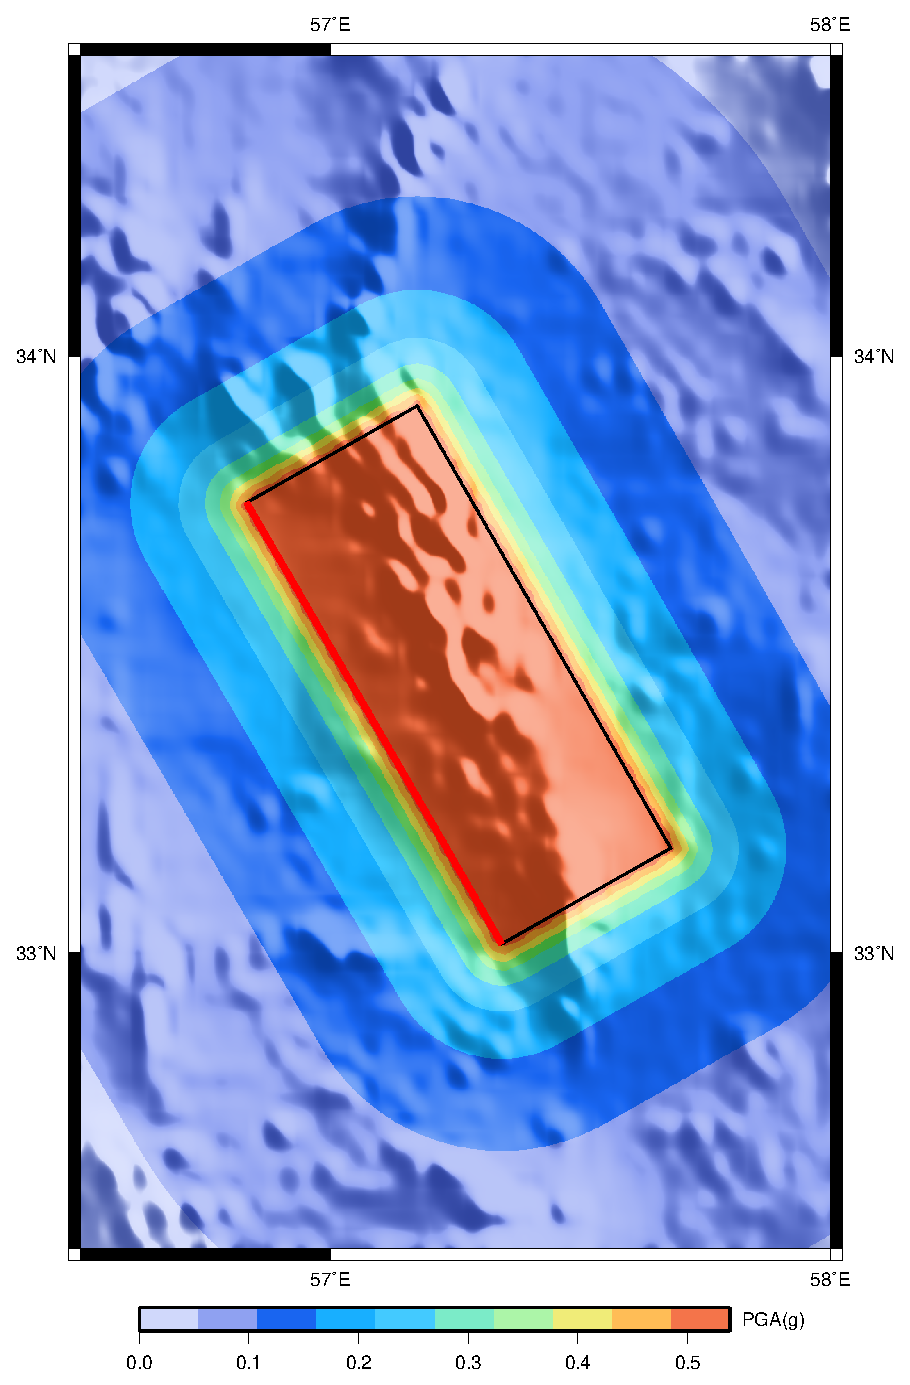
\includegraphics[width=5cm]{./Figures/Part_Hazard/medianGmfTabasPGA.eps}}
\subfigure[]{
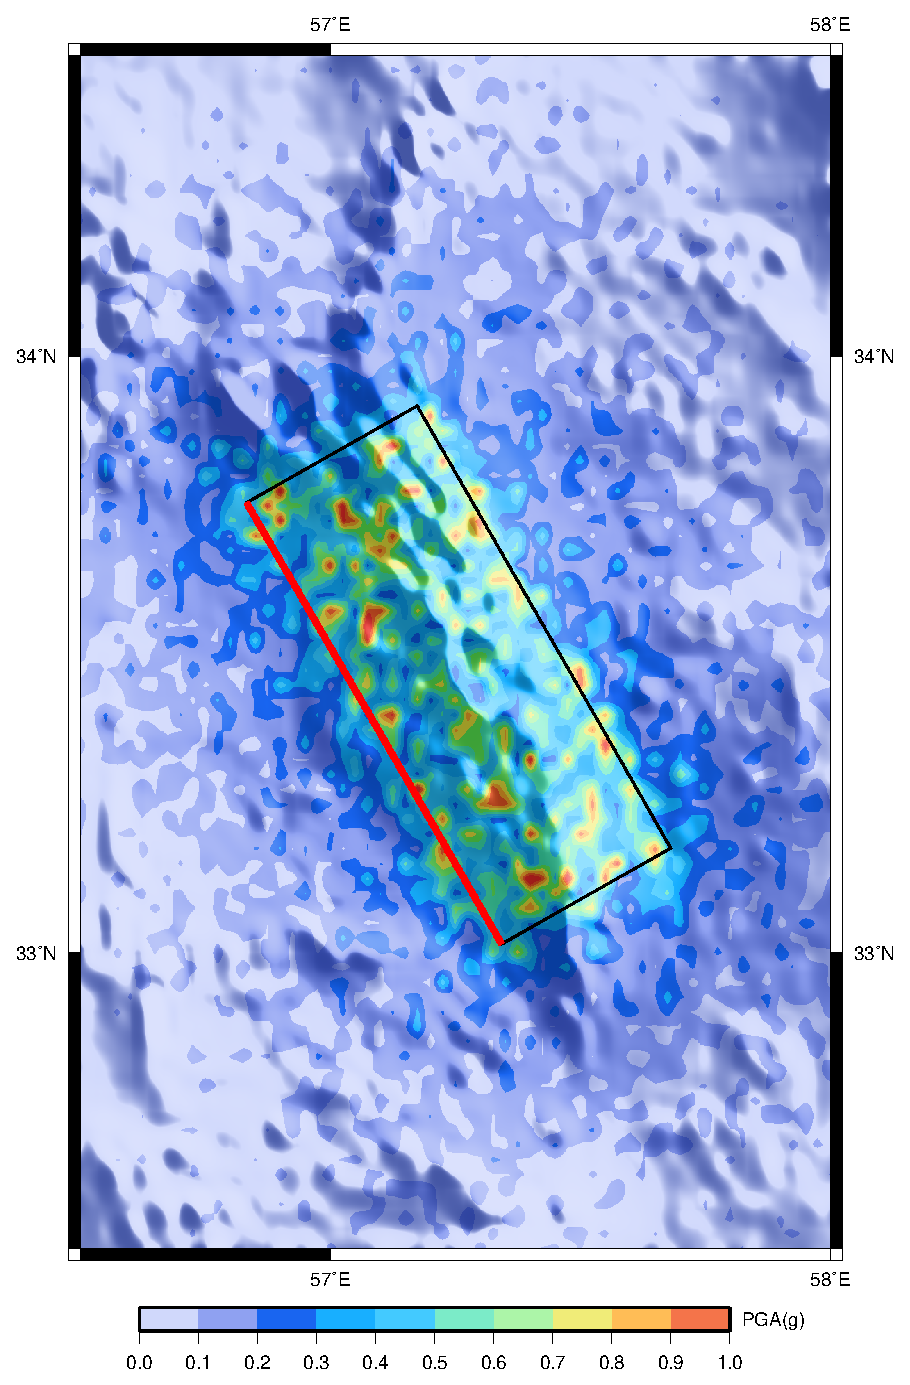
\includegraphics[width=5cm]{./Figures/Part_Hazard/uncorrelatedGmfTabasPGA.eps}}
\subfigure[]{
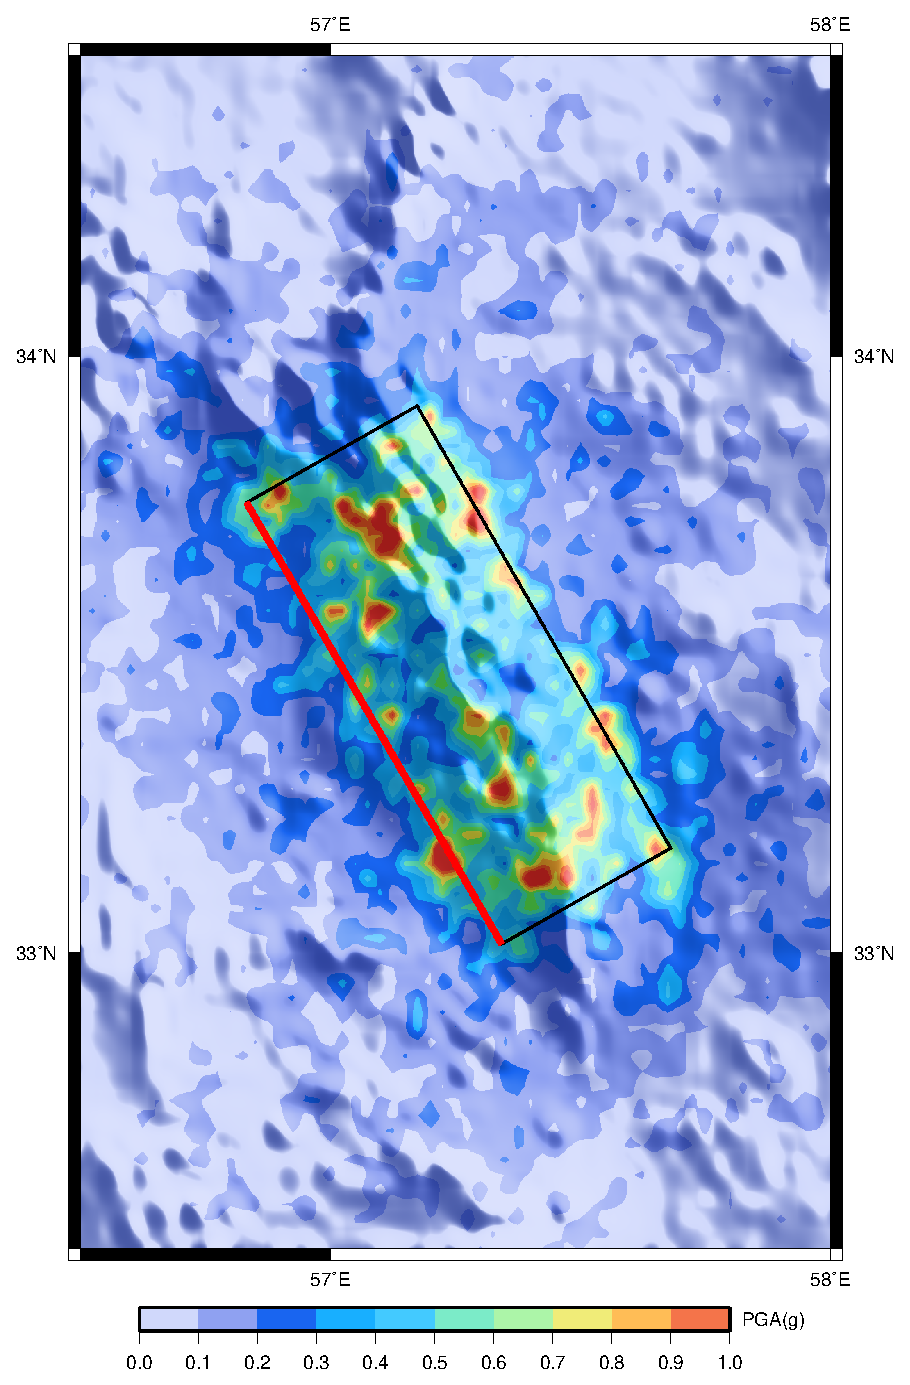
\includegraphics[width=5cm]{./Figures/Part_Hazard/correlatedGmfTabasPGA.eps}}
\subfigure[]{
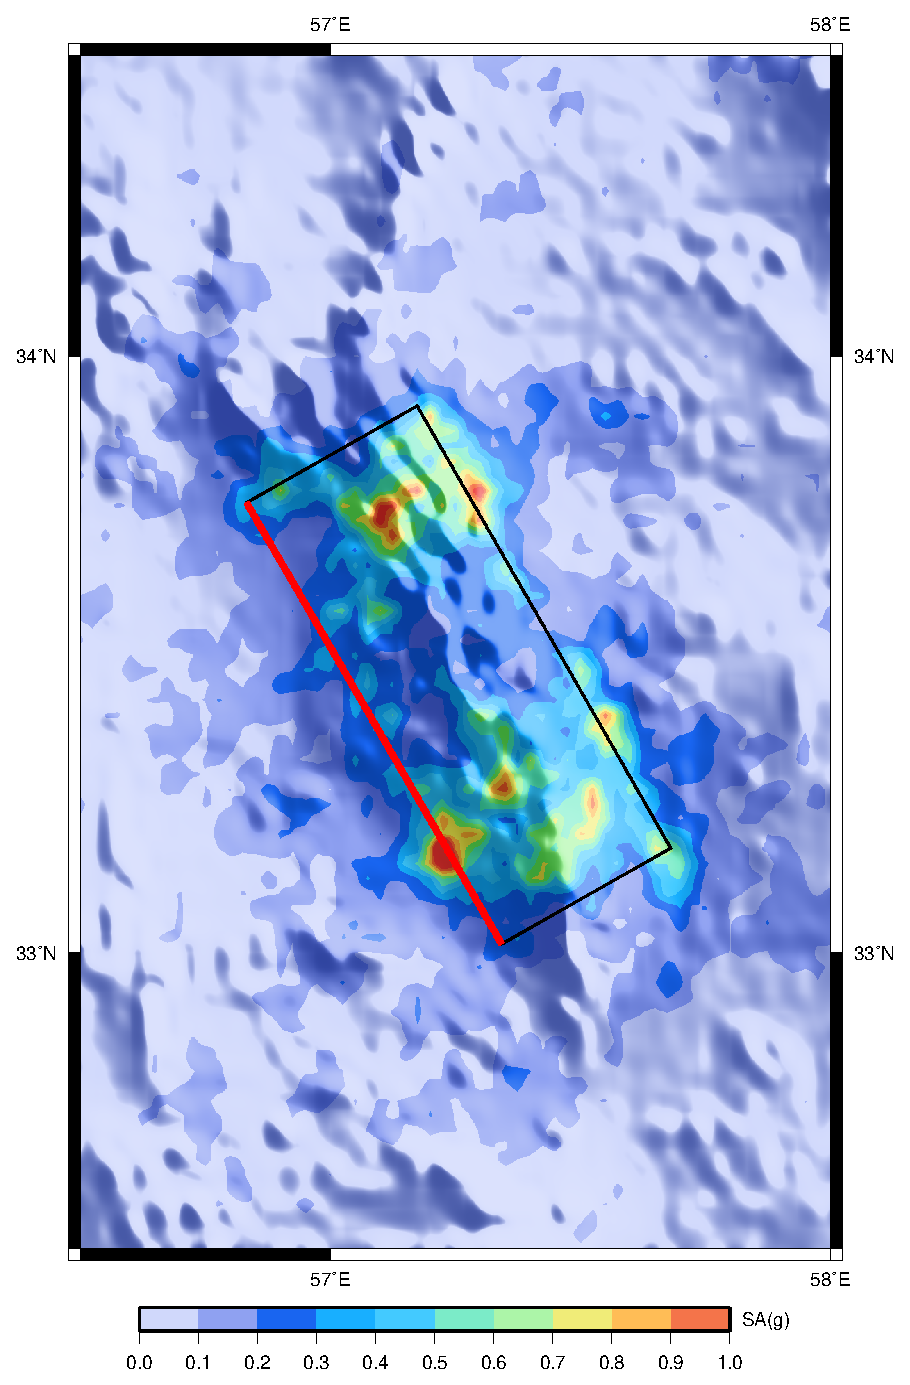
\includegraphics[width=5cm]{./Figures/Part_Hazard/correlatedGmfTabasSA.eps}}
\caption{Examples of median (a), intra-event uncorrelated (b), intra-event 
correlated for PGA (c) and for SA at $T=1$s (d). A rectangular planar rupture 
is considered as source of the shaking (the red line depicts the rupture trace,
and the black line the rupture border). The rupture is associated to a 
magnitude 7 earthquake. The ground-motion is estimated using the 
\citet{boore2008} ground-motion prediction equation.}
\label{fig:gmfs}
\end{figure}

	%
%-------------------------------------------------------------------------------
\clearpage\newpage
\section{PSHA disaggregation}
\label{sec:disaggregation}
%
Seismic hazard disaggregation - or deaggregation - 
\citep{mcguire1995,bazzurro1999} is a procedure aimed at identifying the 
contributions to a specified level of hazard -  referred to a specific site -
coming from different combinations of basic variables - such as magnitude
and rupture-site distance - characterizing the ruptures included in the 
\gls{acr:erf} and the ground motion models selected.
%
Two are the main typologies of disaggregation currently adopted in PSHA 
studies (see for example \citet{petersen2008}): the M-R-$\epsilon$ 
disaggregation and the geographic disaggregation. 
%
Conceptually there are no differences between them; 
simply, in the geographic disaggregation the source-to-rupture 
distance is replaced by the position of the point used to calculate
the distance to the site.
%

In \gls{acr:oq} we introduced a number of new disaggregation typologies 
that should help the modeller in better understanding the PSHA models   
and controlling the results provided for specific sites.
% 
In particular, we added tectonic region and seismic source type to 
the classical disaggregation variables (i.e. magnitude, distance and
epsilon); this way is possible to clearly identify the contribution to 
hazard coming from distinct variables and source/ground motion model
attributes.

The disaggregation methodologies implemented in \gls{acr:oq} is flexible 
enough to provide the best combination possible according to the 
modeller's needs.
% 
\gls{acr:oq} supports disaggregation based on the classical PSHA 
methodology as well as on the event based methodology one. In the 
following sections we describe the details of the approaches
implemented.
%
%- - - - - - - - - - - - - - - - - - - - - - - - - - - - - - - - - - - - - - - -
\subsection{Disaggregation methodology}
Disaggregation from a calculation point of view, simply consists on 
systematically collecting the contributions (i.e. conditional probabilities
of exceedance) to a selected value of hazard for a specific site coming 
from all the rupture included in an \gls{acr:erf}. 
%
In \gls{acr:oq} we use a multidimensional matrix (called disaggregation
matrix) to store these contributions; this matrix contains indexes for:
\begin{itemize}
\item Magnitude (index i)
\item Longitude (index j)
\item Latitude (index k)
\item Source (index s)
\item Epsilon (index l)
\end{itemize}
%
For each rupture the longitude and latitude coordinates is the point 
on the rupture used to calculate the source-site distance.
%
%. . . . . . . . . . . . . . . . . . . . . . . . . . . . . . . . . . . . . . . .
\subsubsection{Classical PSHA: examples of application of the 
disaggregation methodology}
%
In case of the classical PSHA methodology, the cumulation in 
the disaggregation matrix of contributions is based on a 
somewhat modified version of Equation \ref{eq:prob_gm_ex_one_rup}
that distinctly accounts for inputs to the probability of exceedance
of $gm$ coming from different $\epsilon$ intervals.
%
\begin{equation}
P(GM \geq gm|t,rup_{src},\epsilon,site) = 
	P(rup_{src}|t)\,
	P(GM\geq gm|rup_{src},\epsilon,site)
\label{eq:prob_gm_ex_one_rup_eps}
\end{equation}
%
This equation is used recursively to store in the appropriate 
cell the contribution coming from all the ruptures included in 
\gls{acr:erf}. 
%
%
\paragraph{Disaggregation in terms of tectonic region}
The disaggregation in terms of tectonic region is probably the simplest 
disaggregation from a conceptual point of view. 
\begin{multline}
P(GM \geq gm|t,site) = \\
	1-\prod\limits_{\forall\,src\,\text{in}\,ERF}^{}  
	\left\{
		1-\sum\limits_{\forall\,rup\,\text{in}\,src}^{}
		\biggl[ 
			1-\sum\limits_{\forall\,\epsilon}^{} 
			P(GM \geq gm|t,rup_{src},\epsilon,site)
		\biggr]
	\right\}
\label{eq:disaggregation_kernel}
\end{multline}
%

%
%
\paragraph{Disaggregation in terms of tectonic region, magnitude,
distance and epsilon}


%
%. . . . . . . . . . . . . . . . . . . . . . . . . . . . . . . . . . . . . . . .
\subsubsection{Event based PSHA: examples of application of the 
disaggregation methodology}
%
In case of the event-based PSHA methodology the disaggregation consist 
on the cumulation of the events with specific characteristics. 

% ------------------------------------------------------------------------------
%\chapter{Wesson et al. [2009] risk calculation implementation}
%	\input{./Part_Hazard/wessonMethod.tex}
% ==============================================================================
% ------------------------------------------------------------------------- Part
\part{Risk}
% ------------------------------------------------------------------------------
\chapter{Introduction}
	\label{chap:intrisk}
	Introduction to risk calculations
%
% ------------------------------------------------------------------------------
\section{OpenQuake-risk: main concepts}
Blah
%
% ------------------------------------------------------------------------------
\section{Calculation workflows}
The OpenQuake-Risk module offers the capability to perform seismic hazard 
analysis (SHA) following various approaches. Currently three main types of 
analysis are supported:
\begin{itemize}
\item \textbf{Classical PSHA-Based Risk}, 
\item \textbf{Probabilistic Event-Based Risk}, 
\item \textbf{Deterministic Event-Based Risk}, 
\end{itemize}

%
% ------------------------------------------------------------------------------
\chapter{OpenQuake Input Description}
	\label{chap:riskinput}
	The main sources of input information required for a risk calculation with OpenQuake are an exposure model and a physical vulnerability model (in addition to the calculation type, such as those described in Chapter \ref{chap:intrisk}, and the region of interest). An exposure model for a given asset category describes, at each location of interest within a given region, the value of each asset typology. The physical vulnerability model describes the vulnerability characteristics of each asset typology.
%_________________________________________________________
\section{Exposure}
\index{Exposure}
The OpenQuake engine requires an exposure model that needs to be stored according to the respective NRML schema. This file format can include several typologies of asset such as population or buildings. The following parameters are currently being used to describe each asset in the exposure model: 

\begin{itemize}
\item Asset reference: A unique key used to identify the asset instance;
\item Location: Geographic coordinates of the asset expressed in decimal degrees;
\item Asset value: Numerical value of the quantity of the asset at the given location;
\item Vulnerability function: Code of the physical vulnerability function that should be employed in the calculations;
\item Taxonomy: Reference to the classification code that describes the asset.
\end{itemize}

This list of parameters will be further extended in future releases of OpenQuake once more complex data will need to be stored (e.g. value of contents or number of occupants per building at different times of the day).  Furthermore, the definition of the vulnerability function to be used for each asset will be removed from the exposure model, and will instead be stored within a separate file; the two will be linked through the GEM Taxonomy (that is currently under development).

\section{Physical Vulnerability}
\index{Physical Vulnerability}
Physical vulnerability is defined as the probability distribution of loss, given an intensity measure level. These vulnerability functions can be derived directly, usually through empirical methods where the losses from past events at given locations are related to the levels of intensity of ground motion at those locations, or they can be derived by combining fragility functions and consequence functions. Fragility functions describe the probability of exceeding a set of limit states, given an intensity measure level; limit states describe the limits to performance levels, such as damage or injury levels. Fragility functions can be derived by expert-opinion, empirically (using observed data), or analytically, by explicitly modeling the behavior of a given asset typology when subjected to increasing levels of ground motion. Consequence functions describe the probability distribution of loss, given a performance level and are generally derived empirically. 

Version 0.4 of OpenQuake only supports physical vulnerability through the aforementioned vulnerability functions. As part of the Modeller's Toolkit development, calculators that combine fragility functions and consequence functions to produce vulnerability functions will be produced in the future. Furthermore, the possibility to input fragility functions directly is planned in future releases of OpenQuake such that users can view intermediate results of seismic loss calculations, such as the distribution of damage. 

\subsection{Vulnerability Functions}
\subsubsection{Discrete Vulnerability Functions}
\index{Physical Vulnerability!Discrete Functions}
In the current version of OpenQuake (V0.4) discrete vulnerability functions are used to directly estimate fatalities and economic losses due to physical damage. Discrete vulnerability functions are described by a list of intensity measure levels and corresponding mean loss ratios (the ratio of mean loss to exposed value), associated coefficients of variation and probability distributions. The uncertainty on the loss ratio is assumed in OpenQuake v0.4 to follow a lognormal distribution, however different probabilistic distributions for the uncertainty will be developed in future versions, such as the beta distribution. Figure \ref{fig:VFDiscrete} illustrates a discrete vulnerability function.

\begin{figure}[ht]
\centering
\includegraphics[width=10cm,height=6cm]{./Figures/Part_Risk/VFDiscrete.eps}
\caption{Discrete vulnerability function.}
\label{fig:VFDiscrete}
\end{figure}

\subsubsection{Continuous Vulnerability Functions}
\index{Physical Vulnerability!Continuous Functions}
\marginpar{Continuous vulnerability functions are not currently implemented in OQ}
Continuous vulnerability functions will be implemented in future versions of OpenQuake. Continuous vulnerability functions will probably be described by continuous distributions of mean loss ratio and other fractiles of loss ratio, with ground motion intensity. Figure \ref{fig:VFContinuous} illustrates this type of function, showing the distribution of mean loss and the 10 percent and 90 percent fractiles.

\begin{figure}[ht]
\centering
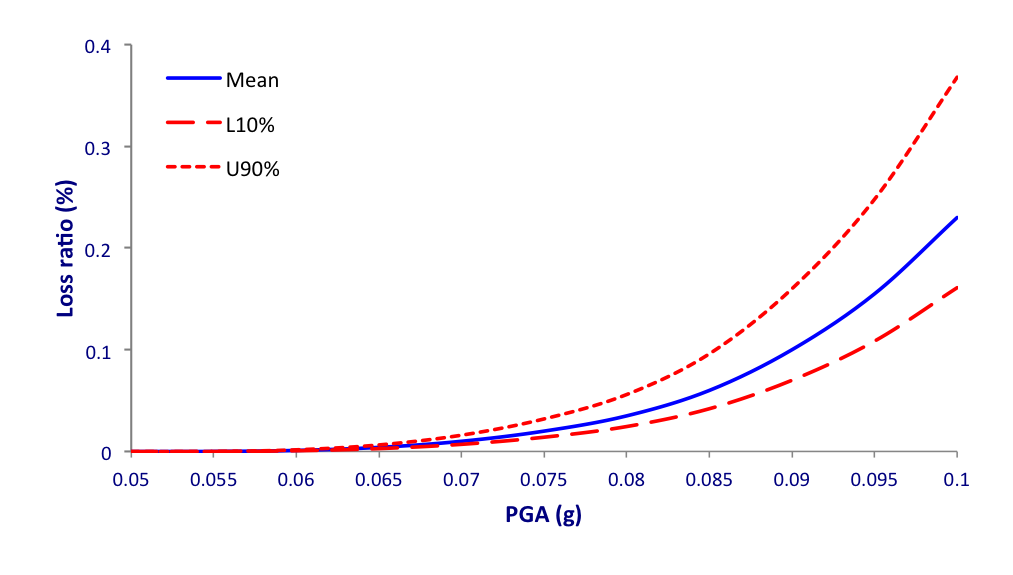
\includegraphics[width=10cm,height=6cm]{./Figures/Part_Risk/VFContinuous}
\caption{Continuous vulnerability function.}
\label{fig:VFContinuous}
\end{figure}

\subsection{Fragility Functions}
\index{Fragility}
\marginpar{Fragility functions are not currently implemented in OQ}
Fragility functions describe the probability of exceeding a set of limit states, given an intensity measure level. When the asset category concerns structures (e.g. buildings), the intensity measure can either be structure-independent or structure-dependent. The former can be calculated directly from recorded measurements of ground shaking (e.g. peak ground acceleration, peak ground velocity, spectral acceleration at a given period of vibration, or even macroseismic intensity). The latter requires information on the characteristics of the structures in order to be calculated, for example spectral acceleration at the fundamental period of vibration, or spectral displacement at the limit state period of vibration. The calculation of these structural characteristics might be through a simple formula (e.g. a yield period-height equation, see e.g. \citet{CrowleyPinho2004} ) or through so-called non-linear static methods, which are needed when the intensity measure is a non-linear response quantity such as spectral displacement at the limit state period of vibration (see e.g. \citet{FEMA440ATC2005}).
Discrete and continuous fragility functions with structure-independent and structure dependent intensity measures (and the methods necessary to calculate them) are not currently supported, but they will be implemented in future versions of OpenQuake. 

\subsubsection{Discrete Fragility Functions}
\index{Fragility!Discrete Functions}
Fragility functions can be defined in a discrete way by providing, for each limit state, a list of intensity measure levels and respective probabilities of exceedance. Figure \ref{fig:FFDiscrete} presents a set of discrete fragility functions using a macroseismic intensity measure. As mentioned previously, these are not yet supported by OpenQuake.

\begin{figure}[ht]
\centering
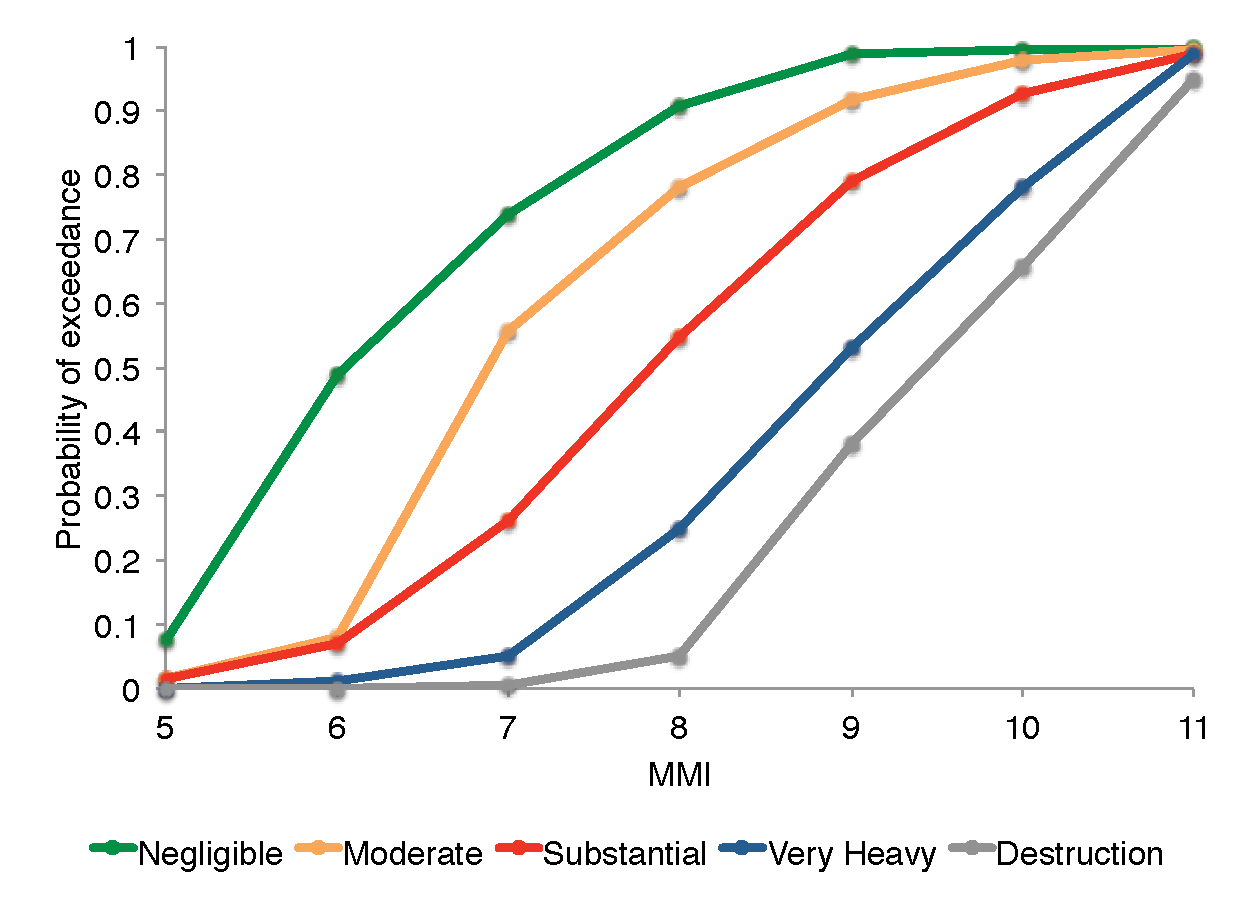
\includegraphics[width=10cm,height=6cm]{./Figures/Part_Risk/FFDiscrete.eps}
\caption{Set of discrete fragility functions.}
\label{fig:FFDiscrete}
\end{figure}

\subsubsection{Continuous Fragility Functions}
\index{Fragility!Continuous Functions}
Continuous fragility functions are defined by the parameters of a cumulative distribution function. In Figure \ref{fig:FFcontinuous} an example of a set of continuous fragility functions with a structure-dependent intensity measure is presented. As mentioned previously, these are not yet supported by OpenQuake.

\begin{figure}[ht]
\centering
\includegraphics[width=10cm,height=6cm]{./Figures/Part_Risk/FFContinuous.eps}
\caption{Set of continuous fragility functions.}
\label{fig:FFcontinuous}
\end{figure}

\subsubsection{Uncertainty in Fragility Functions}
\index{Fragility!Uncertainty}
The uncertainty in continuous fragility functions will also be accounted for in future versions of OpenQuake. Figure \ref{fig:FF_uncertainty} shows a lognormal distribution that has been fit to the data (i.e. the fragility function), and the probabilistic distribution (i.e. mean and standard deviation) to describe the uncertainty in both the logarithmic mean and logarithmic standard deviation of the fragility function. When a set of fragility functions for different limit states are used, it is also necessary to provide information on the correlation between the logarithmic means and logarithmic standard deviations of each limit state.

\begin{figure}[ht]
\centering
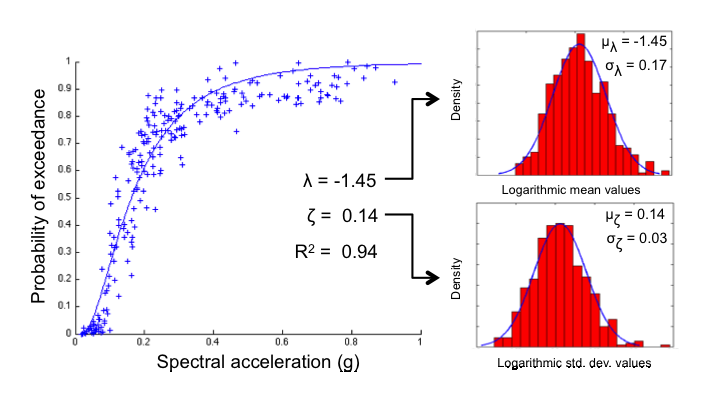
\includegraphics[width=12cm,height=6cm]{./Figures/Part_Risk/FFuncertainty.eps}
\caption{Uncertainty of continuous fragility functions.}
\label{fig:FF_uncertainty}
\end{figure}

\subsection{Consequence Functions}
\index{Consequence Functions}
\marginpar{Consequence functions are not currently implemented in OQ}
Consequence functions describe the probability distribution of loss, given a performance level. For example, if the asset category is buildings and the performance level is significant damage, the consequence function will describe the mean loss ratio, coefficient of variation and probability distribution for that level of damage. Figure \ref{fig:ConsequenceFunctions} presents the mean damage ratios for a set of performance levels proposed by two different sources. 

\begin{figure}[Ht]
\centering
\includegraphics[width=10cm,height=6cm]{./Figures/Part_Risk/ConsequenceFunction.eps}
\caption{Consequence functions adapted from  \citet{Baletal2010}}
\label{fig:ConsequenceFunctions}
\end{figure}


% ------------------------------------------------------------------------------
\chapter{Deterministic Event-Based Risk Calculator}
	\label{chap:risk_deterministic}
	\input{./Part_Risk/Deterministic_Event_Based.tex}
% ------------------------------------------------------------------------------
\chapter{Probabilistic Event-Based Risk Calculator}
	\label{chap:risk_prob_event_based}
	\input{./Part_Risk/Probabilistic_Event_Based.tex}
% ------------------------------------------------------------------------------
\chapter{Classical PSHA-Based Risk Calculator}
	\label{chap:risk_psha_based}
	\input{./Part_Risk/Classical_PSHA_Based.tex}
% ==============================================================================
% ------------------------------------------------------------------------- Part
%\part{Socio-Economic Impact Assessment}
%	Probabilistic Seismic Hazard, a methodology largely 
founded on the works of \citet{cornell1968} and \citet{esteva1968}, 
nowadays contains a well established system of methods. 
%
The development of PSHA within the latest four decades did not change much of 
the original concept but made calculations more rigorous and accurate, 
especially with respect to the treatment of uncertainties. 

The evolution of PSHA methodologies proceeded in parallel with the development 
of instrumental seismology and hardware computing power. Computer codes such as
EQRISK \citep{mcguire1976} and the sequential versions of SEISRISK
\citep{bender1982,bender1987} traced the advancement of PSHA calculation within
the last part of the 20th century.

At the present time, the most computationally intensive PSHA models available 
are the ones developed for site-specific PSHA analyses, such as the ones 
performed for special installations or advanced regional PSHA input models 
(e.g. the UCERF2 model, \citet{field2009}) and the one used for large areas 
(e.g. continents or large nations) require powerful calculation facilities 
and sophisticated codes.
%
The computation demand posed by these model derives in the first case from 
the complexity of the input whilst in the second case is the number of sites 
that renders calculations particularly heavy.  

OpenQuake tries to cover this growing requirement for an accessible and 
efficient code for PSHA calculation. It's worth noting that the hazard 
component of OpenQuake leverages from OpenSHA (http://www.opensha.org) - 
an advanced, open-source, Java-based platform for conducting Seismic 
Hazard Analysis - and it is currently developed in collaboration with 
the OpenSHA team.  
%
% ------------------------------------------------------------------------------
\section{OpenQuake-hazard: main concepts}
Schematically, the procedure that OpenQuake follows to compute probabilistic 
seismic hazard is the following:
%
\begin{enumerate}
%
\item \emph{Read the PSHA input model - i.e. the union of the Seismic Sources 
System and the Ground Motion Model System - and calculation 
settings.}
	\index{Seismic Sources!System} %%%%%%
	\index{PSHA!Input model} %%%%%%
	\index{Ground Motion!Model!System} %%%%%%
	
	The \emph{Seismic Sources System} is an object that contains the 
	information necessary to create one or several Seismic Sources Model, 
	eventually by taking into account the epistemic uncertainties. 
	%
	The Seismic Sources System contains:
	\begin{itemize}
	\item One or several \emph{Initial Seismic Sources Models};
	\index{Logic Tree!Seismic sources} %%%%%%
	\item One logic tree - the Seismic Sources Logic Tree - describing 
	epistemic uncertainties connected with the objects and parameters 
	characterizing the Initial Seismic Sources Models.
	\end{itemize}
	
	The Ground Motion Model System is an object that contains the information 
	necessary to create (or use) one or several Ground Motion models, eventually 
	by taking into account the epistemic uncertainties. 
	\begin{itemize}
	\item One or several Ground Motion Models;
	\index{Logic Tree!Ground Motion Model} %%%%%%
	\item One logic tree - the Ground Motion Model Logic Tree - 
	describing epistemic uncertainties connected with the objects and 
	parameters characterizing the selected Ground Motion Models.	
	\end{itemize}

%
\item \emph{Process the logic tree structures to account for epistemic 
uncertainties connected with the seismic sources and the ground motion 
prediction equations and, create Seismic Sources Models and Ground Motion 
Prediction Equations Models}.
	\index{Seismic Sources!Model} %%%%%%
	\index{Ground Motion! Prediction Equations!Model} %%%%%%
	
	A Seismic Sources Model contains the information necessary to create an 
	Earthquake Rupture Forecast (i.e. the probabilistic seismicity occurrence
	model) without con\-sid\-er\-ing any epistemic uncertainty.
	%
	A Ground Motion Prediction E\-qua\-tions Model includes the information 
	necessary to compute hazard using a Seismic Sources Model. 
\item \emph{Compute the hazard considering as many Seismic Sources Models and 
Ground Motion Prediction Equations Models as need to adequately characterize 
uncertainties}.
\item \emph{Post-process the results obtained for distinct calculations}.
\end{enumerate}
%
% ------------------------------------------------------------------------------
\section{Calculation workflows}
% Three types of analysis
The hazard component of OpenQuake-Hazard performs seismic hazard 
analysis (SHA) following various approaches. 
%
Currently three main types of analysis are supported:
\begin{itemize}
\item \textit{Classical Probabilistic Seismic Hazard Analysis (cPSHA)}, 
allowing calculation of hazard curves and hazard maps following 
classical integration procedure 
(\cite{cornell1968}) as formulated by \cite{field2003}).
\item \textit{Event-Based Probabilistic Seismic Hazard Analysis (ePSHA)}, 
allowing calculation of ground motion fields from stochastic event sets.
\item \textit{Deterministic SHA (DSHA)}, allowing calculation of ground motion 
fields from single earthquake rupture scenario.
\end{itemize}
Each type of analysis has a modular structure, thus providing the capability 
of investigating all possible intermediate results. Moreover, each calculator 
can be expanded independently so that more calculation options/methodologies 
can be easily introduced, without affecting the overall calculation workflow.

Indeed each workflow described in the following Sections involves a number 
of calculators, each responsible for a specific task. 
Figures \ref{classical_psha_workflow}, \ref{event_based_workflow}, and 
\ref{deterministic_workflow} schematically depict the different calculation 
workflows.
%
%  - - - - - - - - - - - - - - - - - - - - - - - - - - - - - - - - - - - - - - -
\subsection{Classical Probabilistic Seismic Hazard Analysis}
\label{section:classicalPSHA}
%
Input data for the classical PSHA consist of a PSHA Input Model (PSHAim) that 
is provided together with a set of calculation settings. 
%
Chapter \ref{chap:hazinp} describes extensively the content of a PSHAim and 
in particular the different options for modeling seismogenic sources and the 
option offered to include epistemic uncertainties on both seismicity and 
ground motion models in the form of a logic tree; Chapter \ref{chap:hazinp} 
also incorporates the description of the logic tree structure adopted.
%
% ..............................................................................
% . . . . . . . . . . . . . . . . . . . . . . . . . . . . . . . . . . . > Figure
\begin{figure}[htbp]
\begin{center}
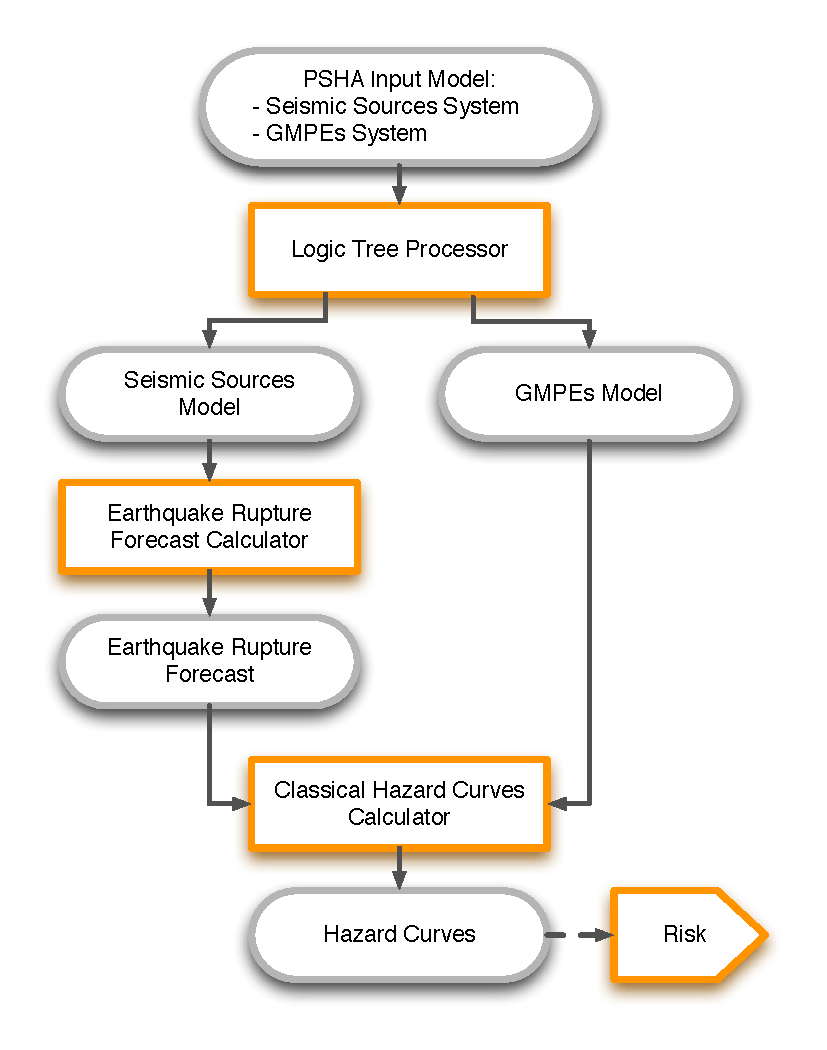
\includegraphics[width=12cm]{./Figures/Part_Hazard/classical_psha_workflow.eps}
\caption{Workflow for classical PSHA (boxes with purple border represent the 
calculators). Given a PSHA Input Model 
the Logic Tree Processor is responsible for creating a Seismic Sources model
and a ground motion model. 
The Seismic Sources model is then provided to the Earthquake Rupture Forecast 
calculator, which computes the ERF (the list of all earthquake ruptures in the 
source model with their probabilities of occurrence). 
Using the ERF and the GMPEs model the Classical PSHA calculator produces 
curves at the sites of interest.}
\label{classical_psha_workflow}
\end{center}
\end{figure}
% . . . . . . . . . . . . . . . . . . . . . . . . . . . . . . . . . . . < Figure
% ..............................................................................

As represented in Figure \ref{classical_psha_workflow}, the main calculators 
used to perform this analysis are:
\begin{enumerate}
%
\item \emph{Logic Tree Processor} \hfill \\
The Logic Tree Processor takes as an input the PSHA Input model. In case of 
the Seismic Sources, using the one of the Initial Seismic Sources Models and 
and by 'harvesting' the information contained in the Seismic Sources Logic Tree
- that is to sample the epistemic uncertainties - it creates a Seismic Sources 
Model (i.e. a model describing geometry and activity rates of each source 
without any epistemic uncertainty). 
%
Following the procedure just described the Logic Tree Processor creates a 
Ground Motion model (i.e. a data structure that associates to each tectonic 
region considered in the calculation a GMPE).
%
\item \emph{Earthquake Rupture Forecast Calculator} \hfill \\
The produced Seismic Sources Model is then used as input for the Earthquake 
Rupture Forecast (ERF) calculator which computes the probability of occurrence, 
over a specified time span, for each earthquake rupture produced by the source 
model.
\item \emph{Classical PSHA Calculator} \hfill \\
The cPSHA uses the ERF and the Ground Motion model to compute hazard curves on 
each site specified in the calculation settings.
\end{enumerate} 
%
%  - - - - - - - - - - - - - - - - - - - - - - - - - - - - - - - - - - - - - - -
\subsection{Event-Based Probabilistic Seismic Hazard Analysis}
\label{section:event-basedPSHA}
Input data for the Event-Based PSHA - as in the case of the Classical PSHA 
calculator - consist of a PSHA Input Model supplied to OQ together with a 
set of calculation settings.
%
% ..............................................................................
% . . . . . . . . . . . . . . . . . . . . . . . . . . . . . . . . . . . > Figure
\begin{figure}
\centering
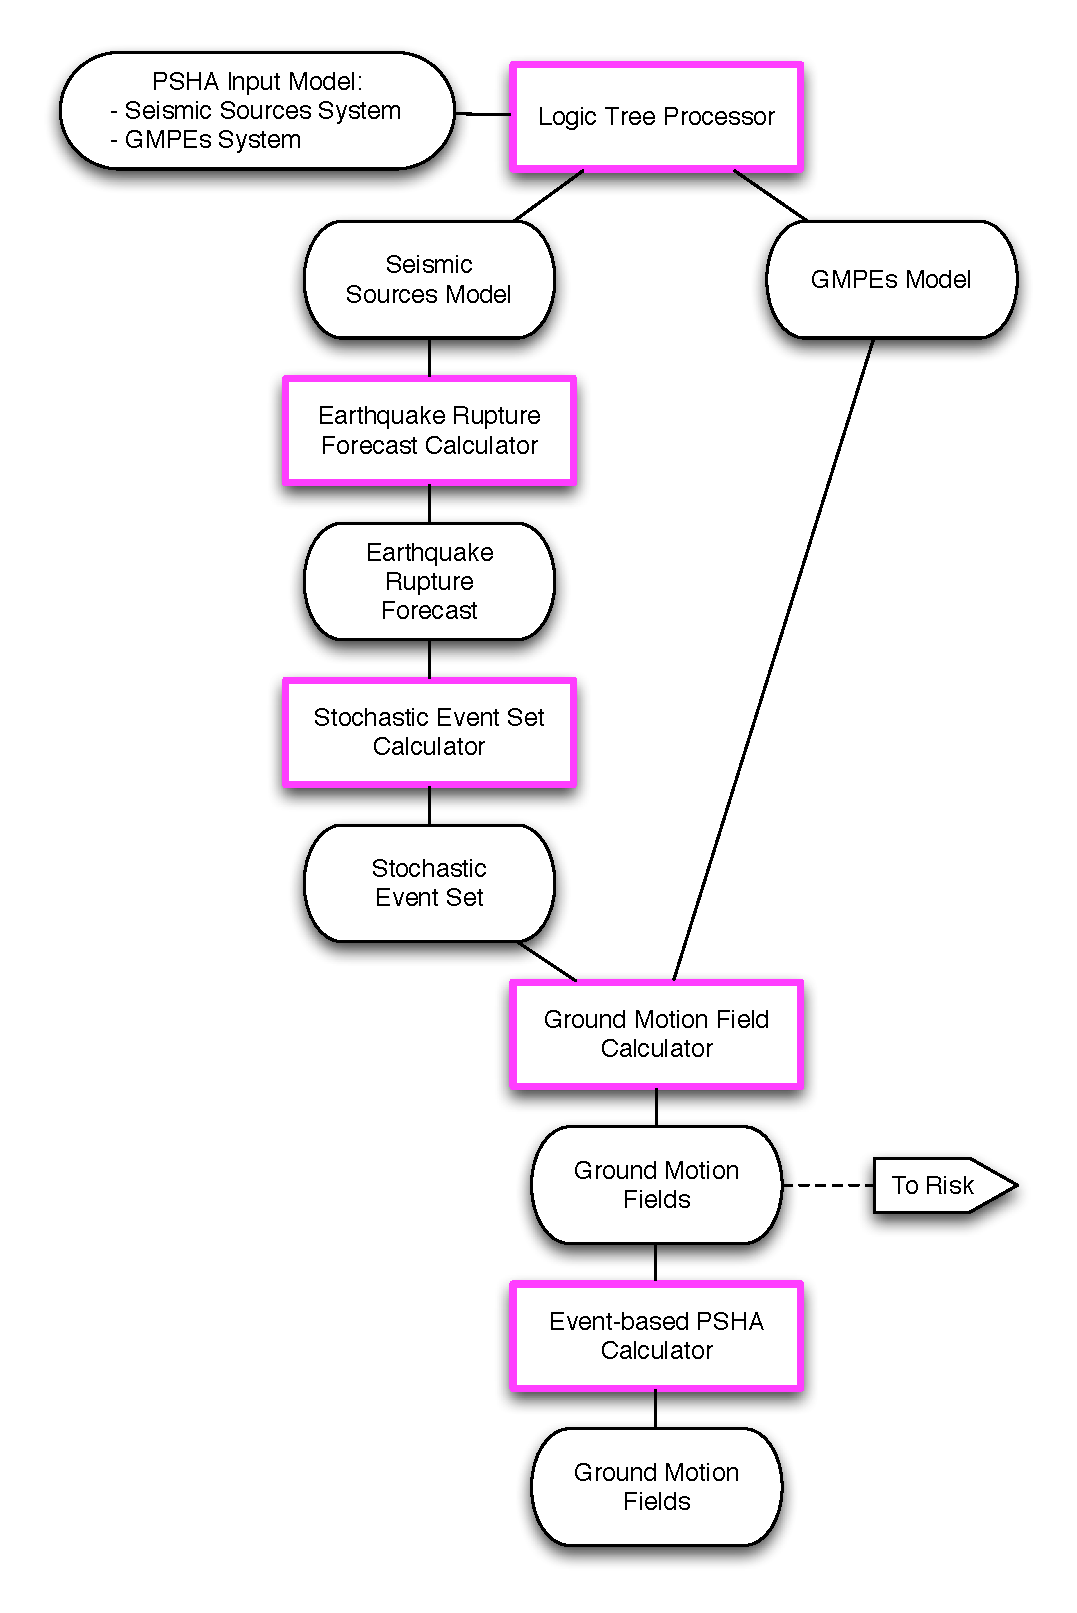
\includegraphics[width=12cm]{./Figures/Part_Hazard/event_based_workflow.eps}
\caption{Workflow for event-based PSHA. Similarly to the classical PSHA workflow 
(Figure \ref{classical_psha_workflow}), an ERF is computed, which is then used 
to generate a stochastic event set (representative of the seismic activity of 
a region in a given time span). Each event is then utilized to calculate a 
ground motion field over a region of interest.}
\label{event_based_workflow}
\end{figure}
% . . . . . . . . . . . . . . . . . . . . . . . . . . . . . . . . . . . < Figure
% ..............................................................................
As represented in Figure \ref{event_based_workflow}, the main calculators 
used to perform this analysis are:
\begin{enumerate}
%
\item \emph{Logic Tree Processor} \hfill \\
The Logic Tree Processor was already 
introduced in the description of the cPSHA workflow (see section 
\ref{section:classicalPSHA} at page \pageref{section:classicalPSHA}).
%
\item \emph{Earthquake Rupture Forecast Calculator} \hfill \\ 
The Logic Tree Processor was already 
introduced in the description of the cPSHA workflow (see section 
\ref{section:classicalPSHA} at page \pageref{section:classicalPSHA}).
%
\item \emph{Stochastic Event Set Calculator} \hfill \\
The Stochastic Event Set Calculator generates a Stochastic Event set 
by sampling each rupture contained in the ERF according to its 
probability of occurrence. Usually a Stochastic Event Set (SES) contains
a large number of seismicity history each one representative of a  
possible collection of events that can be produced by the seismic sources
considered in an analysis during the time span fixed for the calculation
of hazard (normally corresponding to 50 years).
%
\item \emph{Ground Motion Field Calculator} \hfill \\
The Ground Motion Field Calculator computes for each event contained in a 
Stochastic Event Set - provided as an input - a realization of the 
ground shaking taking into account the aleatory uncertainties in 
the ground motion model. Eventually, the Ground Motion Field calculator 
can consider the spatial correlation of the ground motion during the 
generation of the GMF.
%
\item \emph{Event-based PSHA Calculator} \hfill \\
The event-based PSHA calculator takes a (large) set of ground motion 
fields representative of the possible shaking that the investigated 
area can eventually experience over a (large) time span and for each 
grid node in a ground motion fields computes the corresponding hazard 
curve. 
%
This procedure is computationally intensive and is not recommended for 
investigating the hazard over large areas. 
\end{enumerate}

The Logic Tree Processor and the Earthquake rupture forecast were already 
introduced during the descrption of the cPSHA workflow (see section 
\ref{section:classicalPSHA} at page \pageref{section:classicalPSHA}).
%
%  - - - - - - - - - - - - - - - - - - - - - - - - - - - - - - - - - - - - - - -
\subsection{Deterministic Seismic Hazard Analysis}
\label{section:deterministicSHA}
% Deterministic
For deterministic SHA (DSHA), the input data consist of a single earthquake 
rupture model and a single ground motion model. Using the Ground Motion Field 
Calculator, multiple realizations of ground shaking can be computed, each 
realization sampling the aleatory uncertainties in the ground motion model.

As represented in Figure \ref{deterministic_workflow}, the main calculators 
used to perform this analysis are:
\begin{enumerate}
\item \emph{Ground Motion Field Calculator} \hfill \\
The Ground Motion Field Calculator was already 
introduced during the descrption of the ePSHA workflow (see section 
\ref{section:event-basedPSHA} at page \pageref{section:classicalPSHA}).
\end{enumerate}
% ..............................................................................
% . . . . . . . . . . . . . . . . . . . . . . . . . . . . . . . . . . . > Figure
\begin{figure}[!hb]
\centering
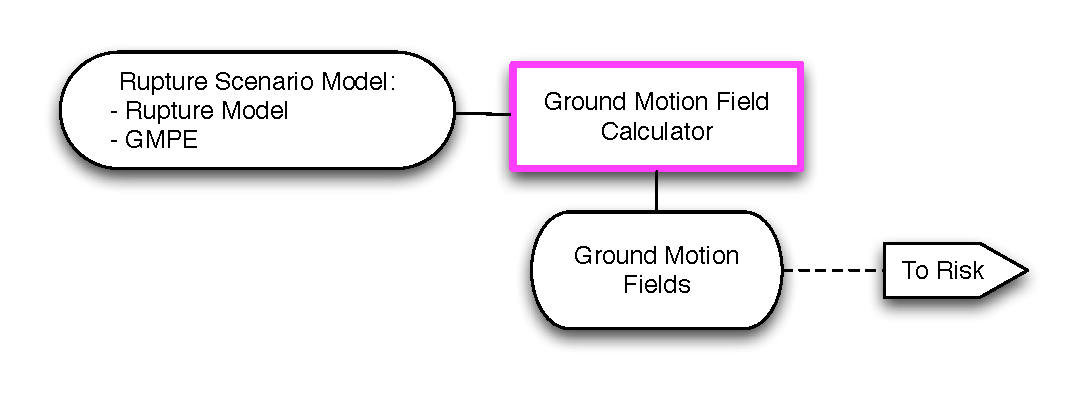
\includegraphics[width=12cm]{./Figures/Part_Hazard/deterministic_workflow.eps}
\caption{Workflow for deterministic SHA. Given a rupture scenario model, 
consisting of an earthquake rupture model, plus a GMPE, the ground motion 
field calculator can compute multiple ground motion field realizations (by 
taking into account GMPE aleatory uncertainties).}
\label{deterministic_workflow}
\end{figure}
% ..............................................................................
% . . . . . . . . . . . . . . . . . . . . . . . . . . . . . . . . . . . > Figure
%
% More details in the next chapters
%Next chapters discuss in more details the data model and the calculators. 
%Chapter \ref{chap:hazinp} describe the input data definition, that is the 
%different options for modeling seismogenic sources and how to include 
%epistemic uncertainties in both seismicity and ground motion models in 
%the form of a logic tree; Chapter \ref{chap:hazinp} also incorporates 
%the description of the logic tree structure adopted. 
%
%The methodology adopted to process the logic tree structure and the 
%definition and modeling of earthquake ruptures for the different 
%seismogenic source typologies are the topics of Chapter \ref{chap:erf}. 
%
%Chapter \ref{chap:hazcalc} describes the theoretical framework behind the main 
%hazard calculator available in OpenQuake: classical PSHA calculator and event 
%based calculator.
% ==============================================================================
% ------------------------------------------------------------------------- Part
%\part{Modeller's Toolkit}
% ------------------------------------------------------------------------------
%\chapter{Introduction}
%	Probabilistic Seismic Hazard, a methodology largely 
founded on the works of \citet{cornell1968} and \citet{esteva1968}, 
nowadays contains a well established system of methods. 
%
The development of PSHA within the latest four decades did not change much of 
the original concept but made calculations more rigorous and accurate, 
especially with respect to the treatment of uncertainties. 

The evolution of PSHA methodologies proceeded in parallel with the development 
of instrumental seismology and hardware computing power. Computer codes such as
EQRISK \citep{mcguire1976} and the sequential versions of SEISRISK
\citep{bender1982,bender1987} traced the advancement of PSHA calculation within
the last part of the 20th century.

At the present time, the most computationally intensive PSHA models available 
are the ones developed for site-specific PSHA analyses, such as the ones 
performed for special installations or advanced regional PSHA input models 
(e.g. the UCERF2 model, \citet{field2009}) and the one used for large areas 
(e.g. continents or large nations) require powerful calculation facilities 
and sophisticated codes.
%
The computation demand posed by these model derives in the first case from 
the complexity of the input whilst in the second case is the number of sites 
that renders calculations particularly heavy.  

OpenQuake tries to cover this growing requirement for an accessible and 
efficient code for PSHA calculation. It's worth noting that the hazard 
component of OpenQuake leverages from OpenSHA (http://www.opensha.org) - 
an advanced, open-source, Java-based platform for conducting Seismic 
Hazard Analysis - and it is currently developed in collaboration with 
the OpenSHA team.  
%
% ------------------------------------------------------------------------------
\section{OpenQuake-hazard: main concepts}
Schematically, the procedure that OpenQuake follows to compute probabilistic 
seismic hazard is the following:
%
\begin{enumerate}
%
\item \emph{Read the PSHA input model - i.e. the union of the Seismic Sources 
System and the Ground Motion Model System - and calculation 
settings.}
	\index{Seismic Sources!System} %%%%%%
	\index{PSHA!Input model} %%%%%%
	\index{Ground Motion!Model!System} %%%%%%
	
	The \emph{Seismic Sources System} is an object that contains the 
	information necessary to create one or several Seismic Sources Model, 
	eventually by taking into account the epistemic uncertainties. 
	%
	The Seismic Sources System contains:
	\begin{itemize}
	\item One or several \emph{Initial Seismic Sources Models};
	\index{Logic Tree!Seismic sources} %%%%%%
	\item One logic tree - the Seismic Sources Logic Tree - describing 
	epistemic uncertainties connected with the objects and parameters 
	characterizing the Initial Seismic Sources Models.
	\end{itemize}
	
	The Ground Motion Model System is an object that contains the information 
	necessary to create (or use) one or several Ground Motion models, eventually 
	by taking into account the epistemic uncertainties. 
	\begin{itemize}
	\item One or several Ground Motion Models;
	\index{Logic Tree!Ground Motion Model} %%%%%%
	\item One logic tree - the Ground Motion Model Logic Tree - 
	describing epistemic uncertainties connected with the objects and 
	parameters characterizing the selected Ground Motion Models.	
	\end{itemize}

%
\item \emph{Process the logic tree structures to account for epistemic 
uncertainties connected with the seismic sources and the ground motion 
prediction equations and, create Seismic Sources Models and Ground Motion 
Prediction Equations Models}.
	\index{Seismic Sources!Model} %%%%%%
	\index{Ground Motion! Prediction Equations!Model} %%%%%%
	
	A Seismic Sources Model contains the information necessary to create an 
	Earthquake Rupture Forecast (i.e. the probabilistic seismicity occurrence
	model) without con\-sid\-er\-ing any epistemic uncertainty.
	%
	A Ground Motion Prediction E\-qua\-tions Model includes the information 
	necessary to compute hazard using a Seismic Sources Model. 
\item \emph{Compute the hazard considering as many Seismic Sources Models and 
Ground Motion Prediction Equations Models as need to adequately characterize 
uncertainties}.
\item \emph{Post-process the results obtained for distinct calculations}.
\end{enumerate}
%
% ------------------------------------------------------------------------------
\section{Calculation workflows}
% Three types of analysis
The hazard component of OpenQuake-Hazard performs seismic hazard 
analysis (SHA) following various approaches. 
%
Currently three main types of analysis are supported:
\begin{itemize}
\item \textit{Classical Probabilistic Seismic Hazard Analysis (cPSHA)}, 
allowing calculation of hazard curves and hazard maps following 
classical integration procedure 
(\cite{cornell1968}) as formulated by \cite{field2003}).
\item \textit{Event-Based Probabilistic Seismic Hazard Analysis (ePSHA)}, 
allowing calculation of ground motion fields from stochastic event sets.
\item \textit{Deterministic SHA (DSHA)}, allowing calculation of ground motion 
fields from single earthquake rupture scenario.
\end{itemize}
Each type of analysis has a modular structure, thus providing the capability 
of investigating all possible intermediate results. Moreover, each calculator 
can be expanded independently so that more calculation options/methodologies 
can be easily introduced, without affecting the overall calculation workflow.

Indeed each workflow described in the following Sections involves a number 
of calculators, each responsible for a specific task. 
Figures \ref{classical_psha_workflow}, \ref{event_based_workflow}, and 
\ref{deterministic_workflow} schematically depict the different calculation 
workflows.
%
%  - - - - - - - - - - - - - - - - - - - - - - - - - - - - - - - - - - - - - - -
\subsection{Classical Probabilistic Seismic Hazard Analysis}
\label{section:classicalPSHA}
%
Input data for the classical PSHA consist of a PSHA Input Model (PSHAim) that 
is provided together with a set of calculation settings. 
%
Chapter \ref{chap:hazinp} describes extensively the content of a PSHAim and 
in particular the different options for modeling seismogenic sources and the 
option offered to include epistemic uncertainties on both seismicity and 
ground motion models in the form of a logic tree; Chapter \ref{chap:hazinp} 
also incorporates the description of the logic tree structure adopted.
%
% ..............................................................................
% . . . . . . . . . . . . . . . . . . . . . . . . . . . . . . . . . . . > Figure
\begin{figure}[htbp]
\begin{center}
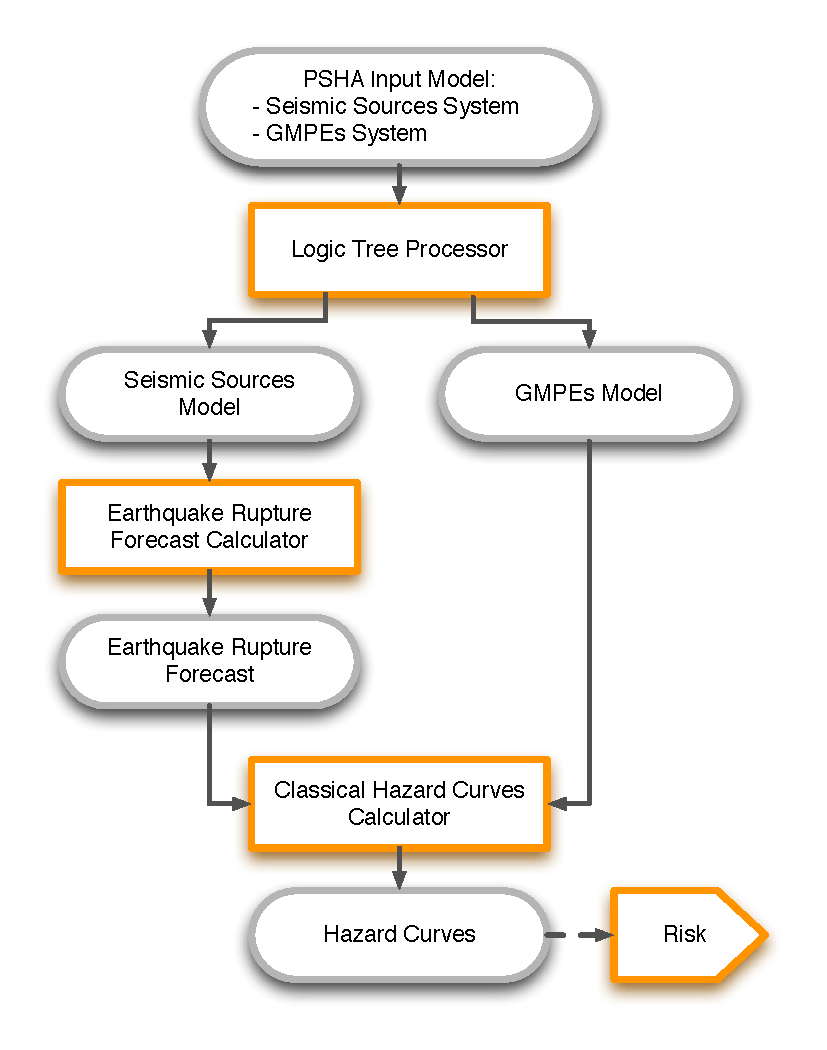
\includegraphics[width=12cm]{./Figures/Part_Hazard/classical_psha_workflow.eps}
\caption{Workflow for classical PSHA (boxes with purple border represent the 
calculators). Given a PSHA Input Model 
the Logic Tree Processor is responsible for creating a Seismic Sources model
and a ground motion model. 
The Seismic Sources model is then provided to the Earthquake Rupture Forecast 
calculator, which computes the ERF (the list of all earthquake ruptures in the 
source model with their probabilities of occurrence). 
Using the ERF and the GMPEs model the Classical PSHA calculator produces 
curves at the sites of interest.}
\label{classical_psha_workflow}
\end{center}
\end{figure}
% . . . . . . . . . . . . . . . . . . . . . . . . . . . . . . . . . . . < Figure
% ..............................................................................

As represented in Figure \ref{classical_psha_workflow}, the main calculators 
used to perform this analysis are:
\begin{enumerate}
%
\item \emph{Logic Tree Processor} \hfill \\
The Logic Tree Processor takes as an input the PSHA Input model. In case of 
the Seismic Sources, using the one of the Initial Seismic Sources Models and 
and by 'harvesting' the information contained in the Seismic Sources Logic Tree
- that is to sample the epistemic uncertainties - it creates a Seismic Sources 
Model (i.e. a model describing geometry and activity rates of each source 
without any epistemic uncertainty). 
%
Following the procedure just described the Logic Tree Processor creates a 
Ground Motion model (i.e. a data structure that associates to each tectonic 
region considered in the calculation a GMPE).
%
\item \emph{Earthquake Rupture Forecast Calculator} \hfill \\
The produced Seismic Sources Model is then used as input for the Earthquake 
Rupture Forecast (ERF) calculator which computes the probability of occurrence, 
over a specified time span, for each earthquake rupture produced by the source 
model.
\item \emph{Classical PSHA Calculator} \hfill \\
The cPSHA uses the ERF and the Ground Motion model to compute hazard curves on 
each site specified in the calculation settings.
\end{enumerate} 
%
%  - - - - - - - - - - - - - - - - - - - - - - - - - - - - - - - - - - - - - - -
\subsection{Event-Based Probabilistic Seismic Hazard Analysis}
\label{section:event-basedPSHA}
Input data for the Event-Based PSHA - as in the case of the Classical PSHA 
calculator - consist of a PSHA Input Model supplied to OQ together with a 
set of calculation settings.
%
% ..............................................................................
% . . . . . . . . . . . . . . . . . . . . . . . . . . . . . . . . . . . > Figure
\begin{figure}
\centering
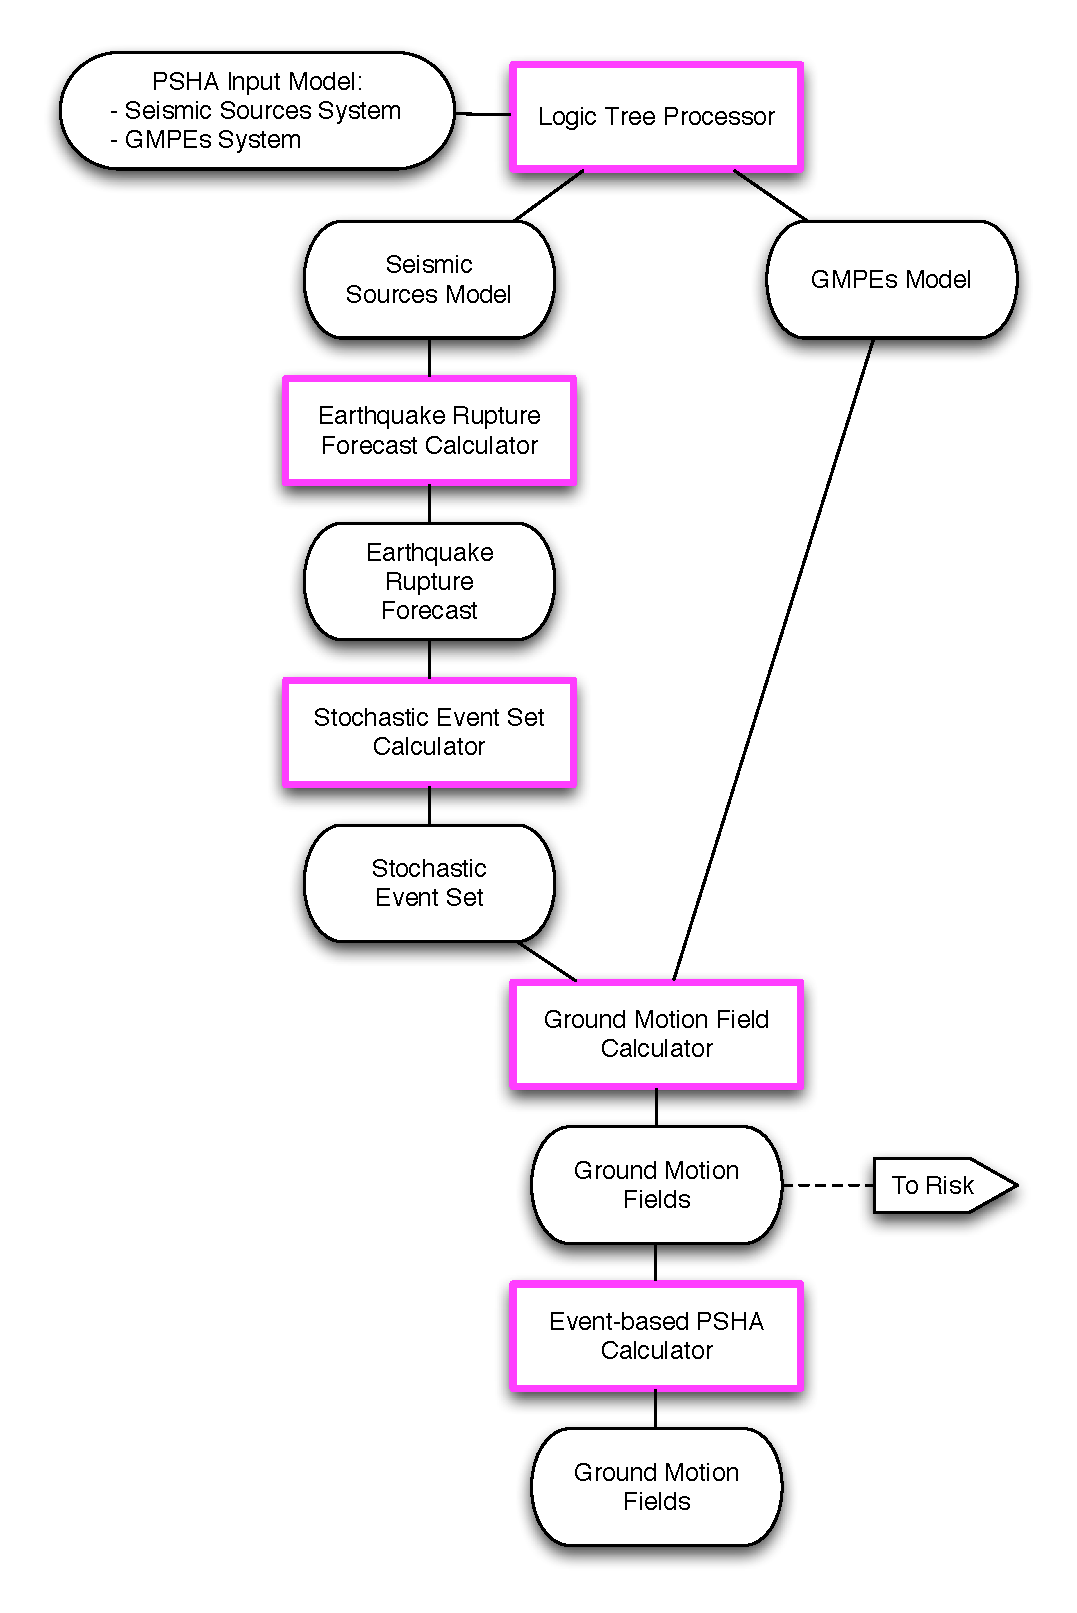
\includegraphics[width=12cm]{./Figures/Part_Hazard/event_based_workflow.eps}
\caption{Workflow for event-based PSHA. Similarly to the classical PSHA workflow 
(Figure \ref{classical_psha_workflow}), an ERF is computed, which is then used 
to generate a stochastic event set (representative of the seismic activity of 
a region in a given time span). Each event is then utilized to calculate a 
ground motion field over a region of interest.}
\label{event_based_workflow}
\end{figure}
% . . . . . . . . . . . . . . . . . . . . . . . . . . . . . . . . . . . < Figure
% ..............................................................................
As represented in Figure \ref{event_based_workflow}, the main calculators 
used to perform this analysis are:
\begin{enumerate}
%
\item \emph{Logic Tree Processor} \hfill \\
The Logic Tree Processor was already 
introduced in the description of the cPSHA workflow (see section 
\ref{section:classicalPSHA} at page \pageref{section:classicalPSHA}).
%
\item \emph{Earthquake Rupture Forecast Calculator} \hfill \\ 
The Logic Tree Processor was already 
introduced in the description of the cPSHA workflow (see section 
\ref{section:classicalPSHA} at page \pageref{section:classicalPSHA}).
%
\item \emph{Stochastic Event Set Calculator} \hfill \\
The Stochastic Event Set Calculator generates a Stochastic Event set 
by sampling each rupture contained in the ERF according to its 
probability of occurrence. Usually a Stochastic Event Set (SES) contains
a large number of seismicity history each one representative of a  
possible collection of events that can be produced by the seismic sources
considered in an analysis during the time span fixed for the calculation
of hazard (normally corresponding to 50 years).
%
\item \emph{Ground Motion Field Calculator} \hfill \\
The Ground Motion Field Calculator computes for each event contained in a 
Stochastic Event Set - provided as an input - a realization of the 
ground shaking taking into account the aleatory uncertainties in 
the ground motion model. Eventually, the Ground Motion Field calculator 
can consider the spatial correlation of the ground motion during the 
generation of the GMF.
%
\item \emph{Event-based PSHA Calculator} \hfill \\
The event-based PSHA calculator takes a (large) set of ground motion 
fields representative of the possible shaking that the investigated 
area can eventually experience over a (large) time span and for each 
grid node in a ground motion fields computes the corresponding hazard 
curve. 
%
This procedure is computationally intensive and is not recommended for 
investigating the hazard over large areas. 
\end{enumerate}

The Logic Tree Processor and the Earthquake rupture forecast were already 
introduced during the descrption of the cPSHA workflow (see section 
\ref{section:classicalPSHA} at page \pageref{section:classicalPSHA}).
%
%  - - - - - - - - - - - - - - - - - - - - - - - - - - - - - - - - - - - - - - -
\subsection{Deterministic Seismic Hazard Analysis}
\label{section:deterministicSHA}
% Deterministic
For deterministic SHA (DSHA), the input data consist of a single earthquake 
rupture model and a single ground motion model. Using the Ground Motion Field 
Calculator, multiple realizations of ground shaking can be computed, each 
realization sampling the aleatory uncertainties in the ground motion model.

As represented in Figure \ref{deterministic_workflow}, the main calculators 
used to perform this analysis are:
\begin{enumerate}
\item \emph{Ground Motion Field Calculator} \hfill \\
The Ground Motion Field Calculator was already 
introduced during the descrption of the ePSHA workflow (see section 
\ref{section:event-basedPSHA} at page \pageref{section:classicalPSHA}).
\end{enumerate}
% ..............................................................................
% . . . . . . . . . . . . . . . . . . . . . . . . . . . . . . . . . . . > Figure
\begin{figure}[!hb]
\centering
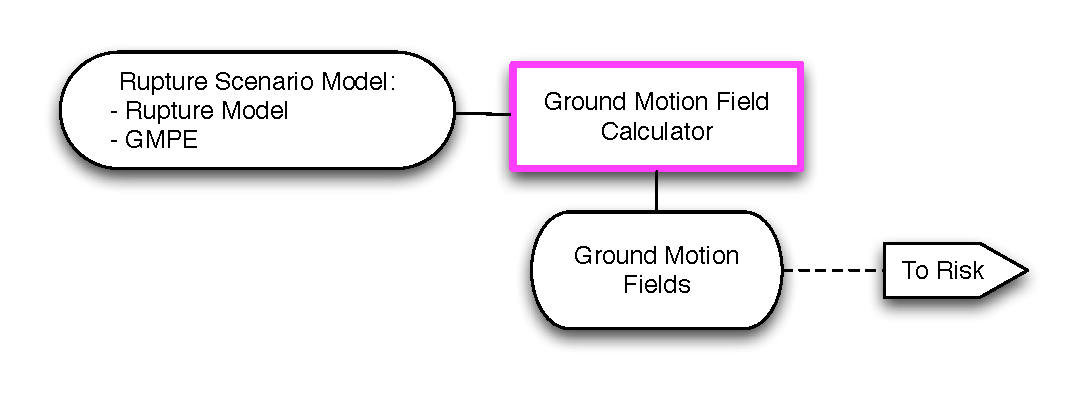
\includegraphics[width=12cm]{./Figures/Part_Hazard/deterministic_workflow.eps}
\caption{Workflow for deterministic SHA. Given a rupture scenario model, 
consisting of an earthquake rupture model, plus a GMPE, the ground motion 
field calculator can compute multiple ground motion field realizations (by 
taking into account GMPE aleatory uncertainties).}
\label{deterministic_workflow}
\end{figure}
% ..............................................................................
% . . . . . . . . . . . . . . . . . . . . . . . . . . . . . . . . . . . > Figure
%
% More details in the next chapters
%Next chapters discuss in more details the data model and the calculators. 
%Chapter \ref{chap:hazinp} describe the input data definition, that is the 
%different options for modeling seismogenic sources and how to include 
%epistemic uncertainties in both seismicity and ground motion models in 
%the form of a logic tree; Chapter \ref{chap:hazinp} also incorporates 
%the description of the logic tree structure adopted. 
%
%The methodology adopted to process the logic tree structure and the 
%definition and modeling of earthquake ruptures for the different 
%seismogenic source typologies are the topics of Chapter \ref{chap:erf}. 
%
%Chapter \ref{chap:hazcalc} describes the theoretical framework behind the main 
%hazard calculator available in OpenQuake: classical PSHA calculator and event 
%based calculator.
% ------------------------------------------------------------------------------
%\chapter{Input visualization and preparation}
%	\input{./Part_Modellers_Toolkit/input.tex}
% ==============================================================================
% ------------------------------------------------------------------------------
% ------------------------------------------------------------------------- Part
%\part{Appendixes}
%\appendix
% ------------------------------------------------------------------------------
%\chapter{nrML}
%	\input{./Part_Appendix/nrML.tex}
% ------------------------------------------------------------------------------
%\chapter{Example of OpenQuake risk calculation configuration file}
%	\input{./Part_Appendix/appendixHazardInputExample.tex}
% ==============================================================================
% ----------------------------------------------------------------- Bibliography
\small
\bibliographystyle{apalike}
\bibliography{./Bibliography/hazard,./Bibliography/risk,./Bibliography/sei.bib}
\normalsize
% ==============================================================================
% ------------------------------------------------------------------------ Index
\printglossaries
\printindex
\cleardoublepage
% Final empty page
\hfill \\ \thispagestyle{empty} \clearpage 
% ==============================================================================
% ------------------------------------------------------------------- Back Cover
\newgeometry{hmargin={0cm,-0.4cm},height=29.7cm}
\thispagestyle{empty}
\psset{unit=1cm}
\begin{pspicture}(0,0)(21cm,29.7cm)
	\psframe[fillstyle=solid,linecolor=gray02,fillcolor=white]
		(0.0cm,0.0cm)(21cm,15.0cm)
	\psframe[fillstyle=solid,linecolor=white,fillcolor=white]
		(0.0cm,15.0cm)(21cm,29.7cm)
	\psframe[fillstyle=solid,linecolor=orange01,fillcolor=orange01]
		(0.0cm,15.0cm)(21cm,15.5cm)
	\psframe[fillstyle=solid,linecolor=orange01,fillcolor=orange01]
		(0.0cm,25.0cm)(21cm,25.1cm)
\end{pspicture}
%
\end{document}
